% ============================================================================
% File: main.tex
% Description: Complete Thai University Laboratory Report Template (Modular)
% Compiler: XeLaTeX
% ============================================================================

\documentclass[a4paper, 12pt]{article}

% ----------------------------------------------------------------------------
% 1. Page Layout Configuration
% ----------------------------------------------------------------------------
\usepackage[
  left   = 1.0in,
  right  = 1.0in,
  top    = 1.5in,
  bottom = 1.5in
]{geometry}
\setlength{\footskip}{0.5in}

% ----------------------------------------------------------------------------
% 2. Core Language & Font Setup
% ----------------------------------------------------------------------------
\usepackage{fontspec}
\usepackage{polyglossia}
\usepackage{fancyhdr}
\usepackage{multirow}
\usepackage{booktabs}

\setdefaultlanguage{thai}
\setotherlanguage{english}

\setmainfont[Scale=1.35, Ligatures=TeX]{TH Sarabun New}
\newfontfamily\thaifont[Scale=1.35, Ligatures=TeX]{TH Sarabun New}
\newfontfamily\thaifonttt[Scale=1.35]{TH Sarabun New}

%% ── Fira Code สำหรับ Code Block ─────────────────────────────────────────────
\setmonofont{Fira Code}[
    Contextuals = Alternate,
    Scale       = 0.78
]

\XeTeXlinebreaklocale "th"
\XeTeXlinebreakskip = 0pt plus 1pt

% ----------------------------------------------------------------------------
% 3. Corrected Font Size Commands
% ----------------------------------------------------------------------------
\newcommand{\sizeTwentyTwo}{\fontsize{16.30}{19.56}\selectfont}
\newcommand{\sizeEighteen}{\fontsize{13.33}{16.00}\selectfont}

% ----------------------------------------------------------------------------
% 4. Typography & Formatting Packages
% ----------------------------------------------------------------------------
\usepackage{indentfirst}
\usepackage{titlesec}
\usepackage{graphicx}
\usepackage{amsmath}
\usepackage{amssymb}   % \mathcal, \mathbb etc.
\usepackage{setspace}

%% ── Citation commands (\citet, \citealt, \citep) ─────────────────────────────
%% natbib รองรับ \citet{key} → "Author (year)"
%%              \citealt{key} → "Author, year"  (ไม่มีวงเล็บ)
%%              \citep{key}   → "(Author, year)"
%% ต้องมีไฟล์ references.bib และรัน: xelatex → bibtex → xelatex → xelatex
\usepackage[authoryear, round]{natbib}

\setlength{\parindent}{1.5cm}
\setstretch{1.0}

\graphicspath{{images/}}

%% ── แก้ Overfull \hbox จากคำภาษาไทยสลับอังกฤษยาว ────────────────────────────
%% emergencystretch อนุญาตให้ TeX ขยาย word spacing ได้อีก 3em ก่อนจะ overfull
\setlength{\emergencystretch}{3em}

% ----------------------------------------------------------------------------
% 5. Code Listing Setup (Listings + Fira Code)
% ----------------------------------------------------------------------------
\usepackage{listings}
\usepackage{xcolor}

\definecolor{codebg}     {gray}{0.96}
\definecolor{codeframe}  {gray}{0.78}
\definecolor{codecomment}{rgb}{0.45, 0.45, 0.45}
\definecolor{codekw}     {rgb}{0.13, 0.29, 0.53}
\definecolor{codestr}    {rgb}{0.63, 0.13, 0.13}
\definecolor{codenumber} {gray}{0.55}

\lstset{
    language         = C,
    basicstyle       = \ttfamily\fontsize{8}{11}\selectfont,
    breaklines       = true,
    breakatwhitespace= true,
    keywordstyle     = \color{codekw}\bfseries,
    commentstyle     = \color{codecomment}\itshape,
    stringstyle      = \color{codestr},
    numberstyle      = \ttfamily\fontsize{6}{8}\selectfont\color{codenumber},
    backgroundcolor  = \color{codebg},
    frame            = single,
    rulecolor        = \color{codeframe},
    numbers          = left,
    stepnumber       = 1,
    numbersep        = 8pt,
    tabsize          = 4,
    showstringspaces = false,
    xleftmargin      = 2.2em,
    framexleftmargin = 1.8em,
    captionpos       = b
}

% ----------------------------------------------------------------------------
% 6. Page Style (เลขหน้ามุมล่างขวา)
% ----------------------------------------------------------------------------
\pagestyle{fancy}
\fancyhf{}
\renewcommand{\headrulewidth}{0pt}
\fancyfoot[R]{\normalsize\thepage}

\fancypagestyle{plain}{
  \fancyhf{}
  \renewcommand{\headrulewidth}{0pt}
  \fancyfoot[R]{\normalsize\thepage}
}

% ----------------------------------------------------------------------------
% 7. Heading Styles (titlesec)
% ----------------------------------------------------------------------------
\titleformat{\section}{\sizeEighteen\bfseries}{\thesection.}{1ex}{}
\titlespacing*{\section}{0pt}{12pt}{6pt}

\titleformat{\subsection}{\normalsize\bfseries}{\thesubsection}{1ex}{}
\titlespacing*{\subsection}{0pt}{10pt}{4pt}

% ============================================================================
\begin{document}
% ============================================================================

% !TeX root = ../main.tex

\begin{titlepage}
    \centering
    \vspace*{1cm}

    % University logo placeholder
    
\includegraphics[width=0.25\textwidth]{university_logo.png}
    \vspace{1cm}

    {\LARGE \textbf{มหาวิทยาลัยเทคโนโลยีพระจอมเกล้าธนบุรี}}\\[0.4cm]
    {\large สถาบันวิทยาการหุ่นยนต์ภาคสนาม}\\[1.5cm]

    {\Large \textbf{รายงานการทดลอง}}\\[0.5cm]
    {\LARGE \textbf{Lab 3 State Estimation}}\\[1cm]

    {\large \textbf{วิชา FRA233 Control Engineering for Robotics}}\\[2cm]

    {\large \textbf{จัดทำโดย}}\\[0.5cm]

    \begin{tabular}{ll}
        นายทัดชัย สุขสราญ          & 67340500016 \\[4pt]
        นายธนดล พูลสระคู            & 67340500017 \\[4pt]
        นายธรรวิทวัส เพ็งนาม        & 67340500018 \\[4pt]
        นายวราวิชญ์ ศิลายงค์         & 67340500036 \\[4pt]
        นายภคิน ศักดิ์สิทธิ์พิทักษ์  & 67340500060 \\[4pt]
        นางสาวศิรินภา สุขบุญส่ง     & 67340500078 \\
    \end{tabular}

    \vfill

    {\large ปีการศึกษา 2568}

\end{titlepage}

\newpage
\pagestyle{plain}
\setcounter{page}{1}

% !TeX root = ../main.tex

\section{การทดลองที่ 1: วัดค่า Spring Constant (\texorpdfstring{$K$}{K})}
\textit{ครอบคลุม Criteria: Part 1 System Modeling --- ออกแบบการทดลองหา $K$, รายงานค่าทางสถิติ (รวม 2 คะแนน)}

%% ─────────────────────────────────────────
\subsection{บทนำ}

ในการสร้างแบบจำลองทางคณิตศาสตร์ของระบบ Mass-Spring-Damper นั้น ค่า Spring Constant หรือ $K$ คือพารามิเตอร์พื้นฐานตัวแรกที่จำเป็นต้องทราบ โดย $K$ คือค่าที่บอกว่าสปริงต้านทานแรงได้มากน้อยเพียงใดต่อหนึ่งหน่วยของการกระจัด ซึ่งอธิบายได้ด้วย Hooke's Law ในรูป $F = Kx$ ค่านี้จะถูกนำไปใช้โดยตรงในการสร้าง State-Space Model และ Equation of Motion ของระบบในการทดลองที่ 4 และ 5 ดังนั้นความแม่นยำของ $K$ จึงส่งผลโดยตรงต่อความถูกต้องของ Kalman Filter ที่จะสร้างขึ้นในภายหลัง

การหาค่า $K$ ทำได้โดยอาศัยหลักการของ Hooke's Law ซึ่งระบุว่าในช่วง Linear Elastic ของสปริง แรงที่กระทำต่อสปริง $F$ จะแปรผันตรงกับระยะที่สปริงยืดหรือหดออกจากตำแหน่งปกติ $x$ โดย $K$ คือความชันของความสัมพันธ์นี้ ในทางปฏิบัติการทดลองนี้จะทำโดยการใส่มวลที่รู้ค่าลงบนสปริงทีละขั้น แล้ววัดระยะกระจัดที่เกิดขึ้นในแต่ละน้ำหนัก จากนั้นนำข้อมูลที่ได้มา Plot กราฟ Force vs.\ Displacement และใช้ Linear Regression หาค่า $K$ จาก Slope ของเส้นตรงที่ได้

อย่างไรก็ตาม ในการรายงานค่า $K$ อย่างน่าเชื่อถือนั้น การวัดเพียงครั้งเดียวไม่เพียงพอ เนื่องจากการทดลองในโลกความเป็นจริงย่อมมีความคลาดเคลื่อนเกิดขึ้นเสมอ ไม่ว่าจะมาจากความไม่สม่ำเสมอของสปริงเอง การอ่านค่าของผู้ทดลอง หรือสปริงที่อาจไม่ได้ตั้งตรงแนวดิ่งอย่างสมบูรณ์ ดังนั้นการทดลองนี้จึงกำหนดให้ทำซ้ำหลายครั้งและใช้วิธีการทางสถิติที่เหมาะสม เช่น ค่าเฉลี่ย ส่วนเบี่ยงเบนมาตรฐาน และค่า $R^2$ ในการประเมินความน่าเชื่อถือของผลลัพธ์ที่ได้

%% ─────────────────────────────────────────
\subsection{วัตถุประสงค์}
\begin{itemize}
    \item เพื่อหาค่า Spring Constant $K$ ของสปริงที่ใช้ในชุดทดลอง Mass-Spring-Damper
    \item เพื่อเลือกและใช้วิธีทางสถิติที่เหมาะสมในการรายงานค่า $K$ อย่างน่าเชื่อถือ
    \item เพื่อยืนยันว่าสปริงทำงานในช่วง Linear Elastic ตาม Hooke's Law
\end{itemize}

%% ─────────────────────────────────────────
\subsection{สมมติฐาน}
\begin{itemize}
    \item ความสัมพันธ์ระหว่างแรงและการกระจัดของสปริงจะเป็นเชิงเส้น (Linear) ในช่วงน้ำหนักที่ทดสอบ
    \item ค่า $K$ ที่ได้จาก Linear Regression จะมีความสม่ำเสมอและค่า $R^2$ สูง
\end{itemize}

%% ─────────────────────────────────────────
\subsection{ตัวแปร}
\begin{enumerate}
    \item \textbf{ตัวแปรต้น (Independent Variable):} มวลที่กระทำต่อสปริง โดยทำการเพิ่มน็อตตัวเมียทีละ 1 ตัว น้ำหนักประมาณตัวละ 38 g (เพิ่มได้สูงสุด 5 ตัว รวมน้ำหนักสูงสุด 190 g)
    \item \textbf{ตัวแปรตาม (Dependent Variable):} ระยะการกระจัด $x$ (m) ที่เกิดขึ้นในแต่ละระดับน้ำหนัก
    \item \textbf{ตัวแปรควบคุม (Control Variables):}
    \begin{itemize}
        \item ชนิดและค่าความแข็งเดิมของสปริงที่ใช้ทดสอบ
        \item อุณหภูมิห้องและสภาพแวดล้อม
        \item ทิศทางการแขวนสปริง (ต้องอยู่ในแนวดิ่งเสมอเพื่อป้องกันแรงเสียดทานด้านข้าง)
        \item ตำแหน่ง Reference เริ่มต้นก่อนทำการโหลดมวล
    \end{itemize}
\end{enumerate}

%% ─────────────────────────────────────────
\subsection{เอกสารและงานวิจัยที่เกี่ยวข้อง}

\subsubsection{กฎของฮุก (Hooke's Law) และข้อสมมติของวัสดุยืดหยุ่นเชิงเส้น}

\paragraph{ความหมายและความสำคัญของกฎของฮุก}

กฎของฮุกเป็นทฤษฎีพื้นฐานทางกลศาสตร์วัสดุที่ใช้อธิบายความสัมพันธ์ระหว่างแรงที่กระทำต่อวัสดุกับการเปลี่ยนรูปที่เกิดขึ้น โดย Robert Hooke ได้เสนอหลักการนี้ในปี ค.ศ.\ 1678 ซึ่งระบุว่า:
\begin{itemize}
    \item ภายในช่วงยืดหยุ่นของวัสดุ (Elastic Region) การเปลี่ยนรูปของวัสดุจะแปรผันตรงกับแรงที่กระทำ
    \item เมื่อแรงที่กระทำเพิ่มขึ้น การยืดตัวหรือการเสียรูปของวัสดุจะเพิ่มขึ้นตามสัดส่วนเดียวกัน
    \item ตราบใดที่วัสดุยังไม่เกินขีดจำกัดการยืดหยุ่น (Elastic Limit) ความสัมพันธ์นี้ยังคงมีผลบังคับใช้
\end{itemize}

\paragraph{ความสัมพันธ์ระหว่างความเค้นและความเครียด}

ความสัมพันธ์ดังกล่าวสามารถอธิบายได้ผ่านสมการทางคณิตศาสตร์ดังนี้
\begin{equation}
    \sigma = E \varepsilon
\end{equation}
โดยที่:
\begin{itemize}
    \item $\sigma$ คือความเค้น (Stress) แรงที่กระทำต่อพื้นที่หนึ่งหน่วย
    \item $\varepsilon$ คือความเครียด (Strain) การเปลี่ยนแปลงรูปร่างสัมพัทธ์ของวัสดุ
    \item $E$ คือมอดูลัสยัง (Young's Modulus) ตัวบ่งบอกความแข็งของวัสดุ
\end{itemize}

หากวัสดุมีค่า Young's Modulus สูง จะสามารถต้านทานการเปลี่ยนรูปได้มากกว่าวัสดุที่มีค่า Young's Modulus ต่ำ

\paragraph{การประยุกต์ใช้กฎของฮุกกับระบบสปริง}

สำหรับระบบสปริง กฎของฮุกสามารถอธิบายในรูปความสัมพันธ์ระหว่างแรงกับการกระจัด ดังสมการต่อไปนี้
\begin{equation}
    F = K x
    \label{eq:hooke}
\end{equation}
โดยที่:
\begin{itemize}
    \item $F$ คือแรงที่กระทำ (หน่วย: นิวตัน)
    \item $K$ คือค่าคงที่ของสปริง (Spring Constant) ตัวแสดงความแข็งของสปริง
    \item $x$ คือระยะยืดตัว (Displacement)
\end{itemize}

สมการนี้แสดงให้เห็นว่า:
\begin{itemize}
    \item การยืดตัวของสปริงมีความสัมพันธ์เชิงเส้นกับแรงที่กระทำ
    \item ค่าความชันของกราฟแรง-การกระจัดสามารถใช้แทนค่าคงที่ของสปริงได้
\end{itemize}

\begin{figure}[htbp]
    \centering
    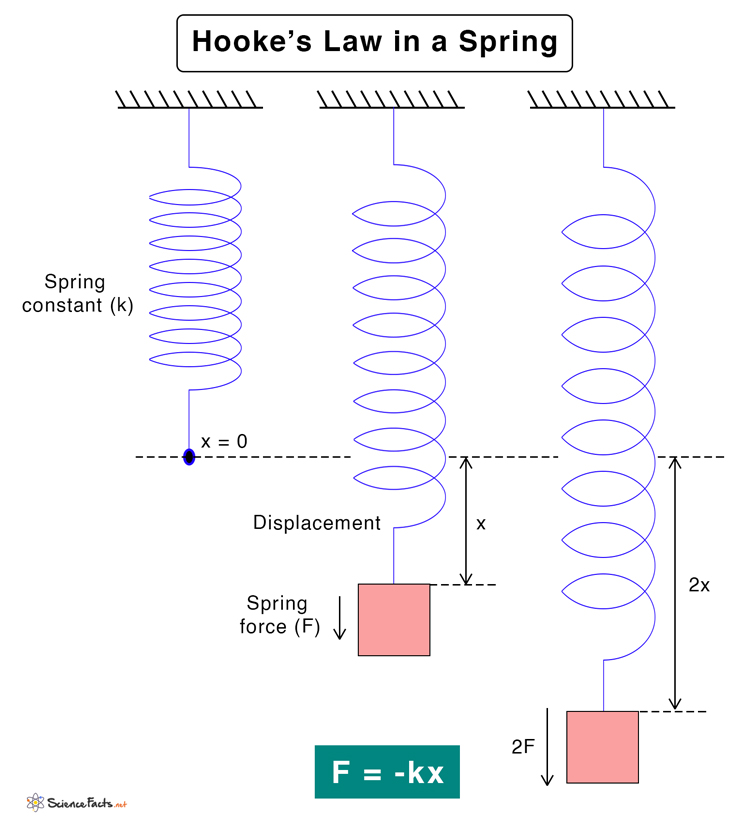
\includegraphics[width=0.6\textwidth]{exp1_hookes_law.jpg}
    \caption{แผนภาพแสดงกฎของฮุก (Hooke's Law)}
    \label{fig:hookes_law}
\end{figure}

\subsubsection{ข้อสมมติของวัสดุยืดหยุ่นเชิงเส้น (Linear Elastic Assumptions)}

\begin{itemize}
    \item \textbf{ข้อสมมติที่ 1 ความสัมพันธ์เชิงเส้นระหว่างความเค้นและความเครียด:} วัสดุต้องมีความสัมพันธ์ระหว่างความเค้นและความเครียดเป็นเชิงเส้น และต้องเป็นไปตามกฎของฮุกอย่างสมบูรณ์ภายในช่วง Elastic Region เท่านั้น
    \item \textbf{ข้อสมมติที่ 2 สมมติการเปลี่ยนรูปเล็กน้อย (Small Deformation Assumption):} การเปลี่ยนรูปของวัสดุต้องมีขนาดเล็กจนสามารถละเลยผลของการเปลี่ยนแปลงทางเรขาคณิตได้
    \item \textbf{ข้อสมมติที่ 3 ความสามารถในการคืนรูป (Reversibility):} วัสดุต้องสามารถคืนรูปได้เมื่อยกเลิกแรงกระทำ ไม่เกิดการเสียรูปถาวร
    \item \textbf{ข้อสมมติที่ 4 สมบัติเชิงกลคงที่:} สมบัติเชิงกลของวัสดุ เช่น Young's Modulus และ Poisson's Ratio ต้องคงที่ตลอดช่วงการรับแรง
    \item \textbf{ข้อสมมติที่ 5 หลักการซ้อนทับ (Superposition Principle):} ผลตอบสนองรวมของระบบที่เกิดจากแรงหลายแรงสามารถหาได้จากผลรวมของผลตอบสนองที่เกิดจากแต่ละแรงแยกกัน
\end{itemize}

\subsubsection{วิธีการทางสถิติ (Statistical Methods)}

\paragraph{ค่าเฉลี่ย (Mean)}

ค่าเฉลี่ยเป็นตัวชี้วัดแนวโน้มเข้าสู่ส่วนกลางของข้อมูล ใช้แสดงค่าตัวแทนของชุดข้อมูลจากการวัดซ้ำ โดยคำนวณจากสมการ
\begin{equation}
    \bar{x} = \frac{1}{N}\sum_{i=1}^{N} x_i
    \label{eq:mean}
\end{equation}
โดยที่ $\bar{x}$ คือค่าเฉลี่ย, $x_i$ คือค่าข้อมูลแต่ละตัว, และ $N$ คือจำนวนข้อมูลทั้งหมด

\paragraph{ส่วนเบี่ยงเบนมาตรฐาน (Standard Deviation)}

ส่วนเบี่ยงเบนมาตรฐานเป็นเครื่องมือที่ใช้วัดการกระจายตัวของข้อมูลจากค่าเฉลี่ย โดยคำนวณได้จากสมการ
\begin{equation}
    s = \sqrt{\frac{\sum_{i=1}^{N}(x_i - \bar{x})^2}{N-1}}
    \label{eq:std}
\end{equation}

\paragraph{สัมประสิทธิ์ความแปรปรวน (Coefficient of Variation: CV)}

สัมประสิทธิ์ความแปรปรวนเป็นอัตราส่วนระหว่างส่วนเบี่ยงเบนมาตรฐานกับค่าเฉลี่ย และแสดงในรูปเปอร์เซ็นต์
\begin{equation}
    CV = \frac{s}{\bar{x}} \times 100\%
    \label{eq:cv}
\end{equation}

\subsubsection{การวิเคราะห์การถดถอยเชิงเส้น (Linear Regression)}

การวิเคราะห์การถดถอยเชิงเส้นเป็นเครื่องมือสำคัญในการศึกษาความสัมพันธ์ระหว่างตัวแปร สมการพื้นฐานของการถดถอยเชิงเส้นสามารถเขียนได้เป็น
\begin{equation}
    y = mx + c
\end{equation}
โดยที่ $y$ คือตัวแปรตาม, $x$ คือตัวแปรอิสระ, $m$ คือความชัน (Slope), และ $c$ คือจุดตัดแกน (Intercept)

สำหรับการทดลองที่เกี่ยวข้องกับกฎของฮุก เมื่อบังคับให้เส้นตรงผ่านจุดกำเนิด (Intercept = 0) สูตร Slope จาก Regression ผ่านจุดกำเนิดคือ
\begin{equation}
    K = \frac{\displaystyle\sum_{i=1}^{n} F_i \cdot \Delta x_i}{\displaystyle\sum_{i=1}^{n} (\Delta x_i)^2}
    \label{eq:regression_slope}
\end{equation}

\paragraph{สัมประสิทธิ์การตัดสินใจ ($R^2$)}

ค่า $R^2$ ใช้วัดระดับความสอดคล้องของข้อมูลกับเส้นแนวโน้ม หากค่า $R^2$ มีค่าเข้าใกล้ 1 (เช่น 0.95 ขึ้นไป) แสดงว่าข้อมูลมีความสัมพันธ์เชิงเส้นที่ดีและสอดคล้องกับแบบจำลองทางทฤษฎี

%% ─────────────────────────────────────────
\subsection{ขั้นตอนการทดลอง}

\begin{enumerate}
    \item ติดตั้งสปริงในแนวดิ่งกับชุดทดลอง จากนั้นกำหนดตำแหน่ง Reference โดยวัดระยะจากปลายสปริงถึงจุดอ้างอิงขณะยังไม่มีโหลดใดๆ บันทึกเป็น $x_\text{ref}$
    \item ใส่น็อตตัวเมียทีละหนึ่งตัวจนครบ 5 ตัว เพราะน้ำหนักสูงสุดที่ใส่ได้คือ น็อต 5 ตัว โดยชั่งมวลน็อตแต่ละชุดสะสมก่อนทดลองเพื่อให้ทราบค่า $m$ ที่แน่นอน แล้วคำนวณแรงกระทำที่แต่ละระดับโหลดด้วย
    \begin{equation}
        F = mg, \quad g = 9.81 \; \text{m/s}^2
        \label{eq:weight}
    \end{equation}
    \item วัดระยะ $x$ จากตำแหน่ง Reference ที่แต่ละระดับโหลด ทำซ้ำ 3 ครั้งต่อระดับโดยถอดและใส่โหลดใหม่ทุกครั้ง เพื่อหาค่าเฉลี่ยและลด Bias จากการอ่านค่าซ้ำในตำแหน่งเดิม บันทึกเป็น $x_1$, $x_2$, $x_3$ และคำนวณการกระจัดสุทธิ
    \begin{equation}
        \Delta x = \bar{x} - x_\text{ref}
        \label{eq:displacement}
    \end{equation}
    \item Plot กราฟ $F$ (แกน $y$) เทียบกับ $\Delta x$ (แกน $x$) และ Fit เส้นตรงผ่านจุดกำเนิด (Intercept = 0) ด้วย Linear Regression เพื่อให้สอดคล้องกับ Hooke's Law: $F = K \cdot \Delta x$
    \item อ่านค่า $K$ จาก Slope ของ Regression Line คำนวณ Mean และ Standard Deviation ของ $K_i$ จาก Point Estimate แต่ละจุด รวมถึงค่า $R^2$ เพื่อยืนยันความเป็นเชิงเส้น
    \begin{equation}
        K_i = \frac{F_i}{\Delta x_i}, \qquad
        \bar{K} = \frac{1}{n}\sum_{i=1}^{n} K_i, \qquad
        S.D.(K) = \sqrt{\frac{\sum(K_i - \bar{K})^2}{n-1}}
        \label{eq:k_stats}
    \end{equation}
    การเลือกใช้ 5 ระดับโหลด (6 จุดข้อมูลรวมจุดกำเนิด) เป็นจำนวนขั้นต่ำที่ทำให้ Linear Regression
มีระดับความเป็นอิสระ (Degree of Freedom) เพียงพอสำหรับการประมาณค่า $K$ และ Intercept 
พร้อมกันโดยไม่เกิด Overfitting อย่างไรก็ตาม หากเพิ่มจำนวนจุดข้อมูลมากขึ้น ค่า Slope ที่ได้จะมี 
Standard Error ลดลง ทำให้ค่า $K$ มีความน่าเชื่อถือสูงขึ้น แต่ต้องแลกกับเวลาและความพยายามในการ
ทดลองที่เพิ่มขึ้นด้วย
\end{enumerate}

% \begin{figure}[htbp]
%     \centering
%     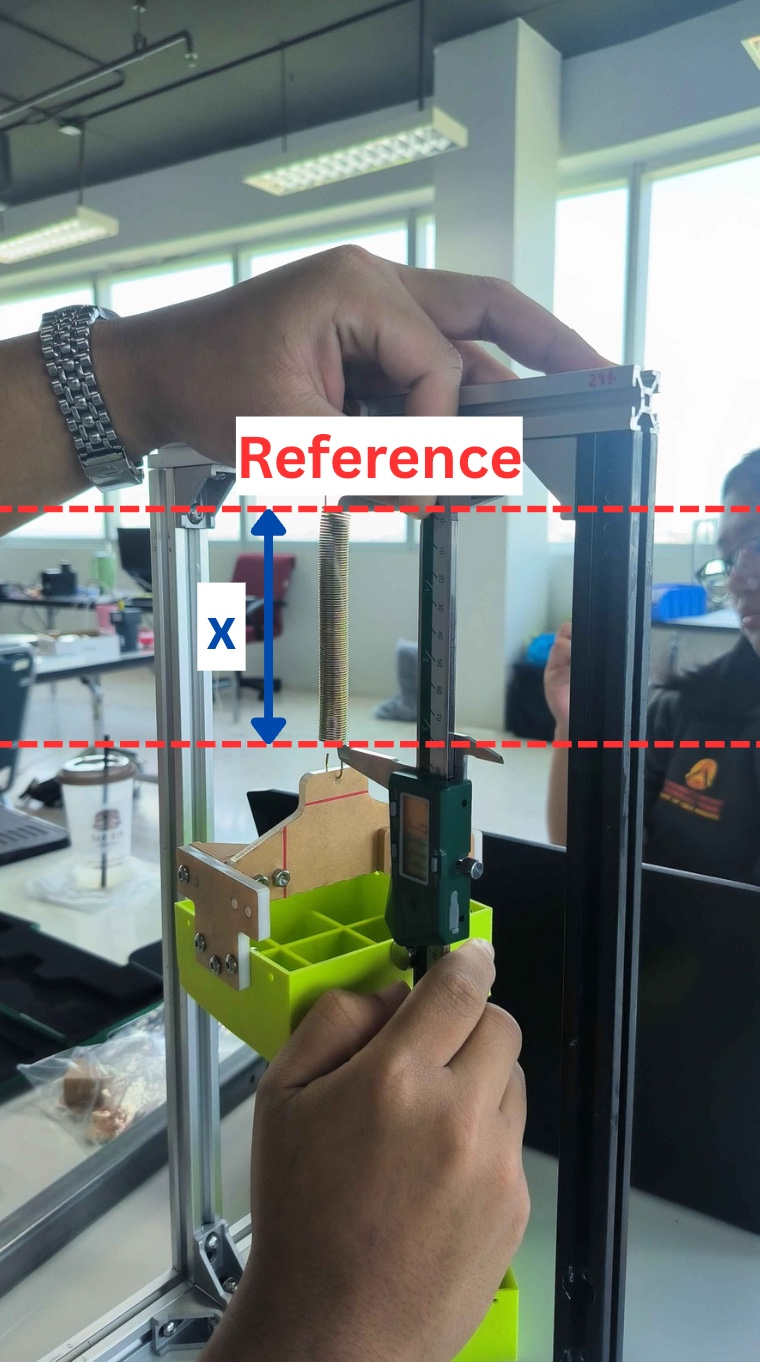
\includegraphics[width=0.35\textwidth]{images/SCR-20260420-octm.jpeg}
%     \caption{ชุดทดลองที่ติดตั้งสปริงในแนวดิ่ง พร้อม Reference Point และตำแหน่งวัด}
%     \label{fig:exp1_setup}
% \end{figure}

%% ─────────────────────────────────────────
\subsection{ผลการทดลอง}

\subsubsection{ตารางข้อมูลที่บันทึกได้}

ตารางด้านล่างแสดงค่าแรงที่กระทำต่อสปริง ($F = mg$) และค่าการกระจัดเฉลี่ย ($\bar{x}$) พร้อมส่วนเบี่ยงเบนมาตรฐาน (S.D.) ที่ได้จากการวัด 3 ครั้งในแต่ละระดับโหลด โดยกำหนดตำแหน่ง Reference ที่ไม่มีโหลดเป็น $x_\text{ref} = 93.272$ mm และคำนวณการกระจัดสุทธิ $\Delta x = \bar{x} - x_\text{ref}$
% การแสดงผลตารางสรุปค่าเฉลี่ยจากการทดลอง
% อ้างอิงหน่วยตามที่ระบุในข้อมูลชุดล่าสุด
\begin{table}[ht]
    \centering
    \caption{ตารางสรุปผลการทดลองหาค่า Spring Constant (เฉพาะค่าเฉลี่ย)}
    \label{tab:spring_summary}
    \begin{tabular}{ccccc}
        \hline
        \textbf{มวลเฉลี่ย $\bar{m}$ (kg)} & \textbf{แรง $F=mg$ (N)} & \textbf{ระยะเฉลี่ย $\bar{x}$ (m)} & \textbf{S.D. ของ $x$ (mm)} & \textbf{S.D. ของ $m$ (g)} \\
        \hline
        % ข้อมูลชุดที่ 1: ตำแหน่งอ้างอิง (No Load)
        0.000 & 0.000 & 0.094 & 0.045 & 0.000 \\
        % ข้อมูลชุดที่ 2: โหลดระดับที่ 1
        0.038 & 0.372 & 0.106 & 1.133 & 0.115 \\
        % ข้อมูลชุดที่ 3: โหลดระดับที่ 2
        0.076 & 0.743 & 0.118 & 1.234 & 0.153 \\
        % ข้อมูลชุดที่ 4: โหลดระดับที่ 3
        0.114 & 1.116 & 0.131 & 1.437 & 0.379 \\
        % ข้อมูลชุดที่ 5: โหลดระดับที่ 4
        0.152 & 1.488 & 0.144 & 0.866 & 0.208 \\
        % ข้อมูลชุดที่ 6: โหลดระดับที่ 5
        0.190 & 1.860 & 0.158 & 1.281 & 0.289 \\
        \hline
    \end{tabular}
        \begin{minipage}{0.85\textwidth}
        \vspace{4pt}
        \footnotesize
        \textit{หมายเหตุ:} ค่า $\bar{x}$ ในตารางนี้แสดงผลแบบ Round เพื่อความกระชับ
        ค่า $\Delta x$ ที่ใช้คำนวณจริงในตารางที่~\ref{tab:k_pointest}
        คำนวณจากข้อมูลดิบก่อน Round ดังนั้นจึงมีทศนิยมมากกว่า
    \end{minipage}
\end{table}

\begin{figure}[htbp]
    \centering
    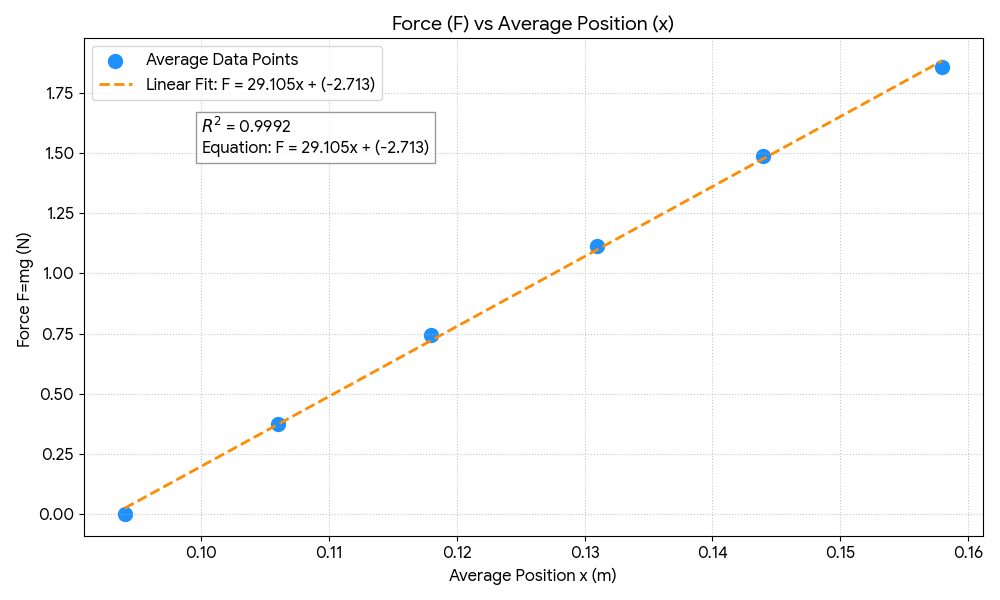
\includegraphics[width=0.75\textwidth]{exp1_force_dist.png}
    \caption{กราฟแสดงผลการทดลองระหว่างแรงกับการกระจัด}
    \label{fig:force_displacement}
\end{figure}

\subsubsection{การคำนวณค่า \texorpdfstring{$K$}{K} ด้วย Linear Regression}

จาก Hooke's Law ความสัมพันธ์ระหว่างแรงและการกระจัดอยู่ในรูป $F = K \cdot \Delta x$
ดังนั้น $K$ คือความชันของเส้นตรง (Slope) ที่ได้จากการทำ Linear Regression
ของข้อมูล Force vs.\ Displacement

ในการวิเคราะห์นี้ใช้สองแนวทาง ได้แก่ \textbf{(1) OLS ผ่านจุดกำเนิด}
ซึ่งตรงกับนิยามของ Hooke's Law โดยตรง และ
\textbf{(2) Full OLS with Intercept} ซึ่งอนุญาตให้มี Offset คงที่
เพื่อรองรับความคลาดเคลื่อนเชิงระบบของการตั้งค่าอุปกรณ์

\paragraph{แนวทางที่ 1: OLS ผ่านจุดกำเนิด}

บังคับให้ Intercept = 0 ตามนิยามของ Hooke's Law ($F = K \cdot \Delta x$)
สูตรที่ใช้คือ
\begin{equation}
    K_{\text{origin}} =
    \frac{\displaystyle\sum_{i=1}^{n} (F_i \cdot \Delta x_i)}
         {\displaystyle\sum_{i=1}^{n} (\Delta x_i)^2}
    = \frac{0.257951}{0.008746}
    \approx 29.49 \; \text{N/m}
\end{equation}

\paragraph{แนวทางที่ 2: Full OLS with Intercept (ค่าที่เลือกใช้)}

เมื่อ Plot กราฟ $F$ vs.\ $\Delta x$ พบว่าเส้น Regression ไม่ผ่านจุดกำเนิดพอดี
แต่มี Offset เล็กน้อย ซึ่งสะท้อนถึง Systematic Error จากการกำหนด Reference
Position ($x_\text{ref}$) ที่มี Measurement Noise เล็กน้อย
จึงใช้ Full OLS ในรูป $F = K \cdot \Delta x + c$ เพื่อจัดการ Offset นี้
\begin{equation}
    \boxed{K = 29.11 \; \text{N/m}} \quad,\quad c = 0.0163 \; \text{N}
\end{equation}
ค่า $K = 29.11$ N/m นี้จะถูกนำไปใช้ในการทดลองที่ 4 และ 5 ทั้งหมด
เนื่องจาก Full OLS ลด Bias จาก Systematic Offset ได้ดีกว่า OLS ผ่านจุดกำเนิด

% --- Section: Spring Constant Analysis ---
\subsection{ผลการวิเคราะห์ค่าคงที่สปริง (Spring Constant Analysis)}

จากการทดลองหาความสัมพันธ์ระหว่างแรง $F$ และระยะยืด $\Delta x$ เพื่อหาค่าคงที่สปริง $K$ ตามกฎของฮุก ($F = k\Delta x$) สามารถสรุปผลการวิเคราะห์เชิงสถิติได้ดังนี้

\subsubsection{การวิเคราะห์ด้วยวิธีการถดถอยเชิงเส้น (Linear Regression)}

จากการวิเคราะห์ใน Section 1.7.2 ด้วย Full OLS ได้ผลลัพธ์:
\begin{equation}
    \boxed{K = 29.11 \; \text{N/m}} \quad,\quad c = 0.0163 \; \text{N}
\end{equation}
เมื่อ $c$ คือ Systematic Offset ของระบบการวัด
ค่า $K = 29.11$ N/m ถูกเลือกเป็นค่าสุดท้ายเนื่องจาก Full OLS
จัดการ Offset ได้ดีกว่า OLS ผ่านจุดกำเนิด (ซึ่งให้ $K_\text{origin} = 29.49$ N/m)

\subsubsection{ค่าทางสถิติและจุดประมาณการ (Point Estimates)}

เพื่อตรวจสอบความสม่ำเสมอของค่าคงที่สปริงในแต่ละช่วงน้ำหนัก จึงคำนวณค่า $K_i$ ณ แต่ละระดับโหลดโดยใช้ความสัมพันธ์ $K_i = F_i / \Delta x_i$ ผลลัพธ์แสดงดังตารางที่ \ref{tab:k_pointest}:

\begin{table}[h]
    \centering
    \caption{ค่า Point Estimate ของ $K$ ที่แต่ละระดับโหลด}
    \label{tab:k_pointest}
    \begin{tabular}{cccc}
        \hline
        \textbf{ระดับโหลด} & \textbf{$F_i$ (N)} & \textbf{$\Delta x_i$ (m)} & \textbf{$K_i$ (N/m)} \\
        \hline
        1 & 0.372 & 0.01222 & 30.44 \\
        2 & 0.743 & 0.02429 & 30.59 \\
        3 & 1.116 & 0.03735 & 29.88 \\
        4 & 1.488 & 0.05007 & 29.72 \\
        5 & 1.860 & 0.06407 & 29.03 \\
        \hline
    \end{tabular}
\end{table}

จากการคำนวณหาค่าเฉลี่ย ($\bar{K}$) และค่าเบี่ยงเบนมาตรฐาน (S.D.) ของกลุ่มตัวอย่าง:
\begin{equation}
    \bar{K} = \frac{\sum_{i=1}^{n} K_i}{n} = 29.93 \; \text{N/m}
\end{equation}
\begin{equation}
    S.D.(K) = \sqrt{\frac{\sum_{i=1}^{n} (K_i - \bar{K})^2}{n-1}} \approx 0.63 \; \text{N/m}
\end{equation}
\textbf{หมายเหตุ:} ค่าเฉลี่ย $29.93$ N/m มีค่าสูงกว่าค่าจากการถดถอยเชิงเส้นเล็กน้อย เนื่องจากการคำนวณรายจุดไม่ได้พิจารณาค่าความคลาดเคลื่อนคงที่ ($c$) ของเครื่องมือวัด

\subsubsection{การคำนวณค่าสัมประสิทธิ์การตัดสินใจ (\texorpdfstring{$R^2$}{R^2})}

เพื่อประเมินความแม่นยำของโมเดล $F = 29.11 \Delta x + 0.0163$ จึงทำการคำนวณค่า $R^2$ สำหรับการถดถอยเชิงเส้น ดังนี้:
\begin{equation}
    R^2 = 1 - \frac{SS_{\text{res}}}{SS_{\text{tot}}} = 1 - \frac{\sum_{i=1}^{n} (F_i - \hat{F}_i)^2}{\sum_{i=1}^{n} (F_i - \bar{F})^2}
\end{equation}
โดยที่ $\hat{F}_i$ คือค่าแรงที่ทำนายจากสมการ และ $\bar{F} = 0.93$ N คือค่าเฉลี่ยของแรงทั้งหมด

\begin{table}[ht]
    \centering
    \caption{ตารางคำนวณ Residuals สำหรับการตรวจสอบค่า $R^2$}
    \label{tab:r2_calc}
    \begin{tabular}{cccccc}
        \hline
        $i$ & $\Delta x_i$ (m) & $F_i$ (N) & $\hat{F}_i$ (N) & $(F_i - \hat{F}_i)^2$ & $(F_i - \bar{F})^2$ \\
        \hline
        1 & 0.00000 & 0.000 & 0.0163 & 0.000266 & 0.8643 \\
        2 & 0.01222 & 0.372 & 0.3721 & 0.000000 & 0.3060 \\
        3 & 0.02429 & 0.743 & 0.7234 & 0.000384 & 0.0347 \\
        4 & 0.03735 & 1.116 & 1.1034 & 0.000159 & 0.0360 \\
        5 & 0.05007 & 1.488 & 1.4740 & 0.000196 & 0.3117 \\
        6 & 0.06407 & 1.860 & 1.8814 & 0.000458 & 0.8655 \\
        \hline
        \textbf{Sum} & & & & \textbf{0.001463} & \textbf{2.4182} \\
        \hline
    \end{tabular}
\end{table}

แทนค่าเพื่อหาผลลัพธ์:
\begin{equation}
    R^2 = 1 - \frac{0.001463}{2.4182} \approx 0.9994
\end{equation}
ค่า $R^2$ ที่เข้าใกล้ 1 ยืนยันว่าสมการเชิงเส้นนี้สามารถอธิบายพฤติกรรมของสปริงได้อย่างครอบคลุม

% --- Section: Discussion and Conclusion ---
\subsection{สรุปและอภิปรายผล}

\begin{itemize}
    \item \textbf{สรุปผล:} เลือกรายงานค่าคงที่สปริง $K = 29.11$ N/m จากวิธี Linear Regression เนื่องจากให้ค่า $R^2 = 0.9994$ ซึ่งแสดงถึงความแม่นยำสูง และสามารถจัดการกับค่า Offset ($c = 0.0163$ N) ของระบบได้ดีกว่าการหาค่าเฉลี่ยรายจุด
    \item \textbf{อภิปรายผล:} ความคลาดเคลื่อน (S.D. $\approx 0.63$ N/m) ส่วนใหญ่เกิดจาก Measurement Noise ในการอ่านค่าระยะยืดด้วยสายตา อย่างไรก็ตาม ค่า $K$ ที่ได้มีความเสถียรเพียงพอสำหรับการนำไปประยุกต์ใช้ใน State-Space Model
    \item \textbf{การนำไปใช้:} ค่า $K = 29.11$ N/m จะถูกนำไปบรรจุลงใน System Matrix ของ Kalman Filter เพื่อใช้ในการพยากรณ์สถานะ (State Prediction) ของระบบมวล-สปริงในการทดลองขั้นต่อไป
\end{itemize}
% !TeX root = ../main.tex
% NOTE: ต้องมี \usepackage{float} ใน preamble ของ main.tex
%       เพื่อให้ [H] float specifier ทำงานได้

\section{การทดลองที่ 2: สร้าง Library HC-SR04 และวัด Measurement Noise Covariance}
% \textit{ครอบคลุม Criteria: Part 2 --- สร้าง Library HC-SR04, หาค่า $R$
% จาก Variance ของ Raw Data (ส่วนหนึ่งของ 5.5 คะแนน)}

%% ─────────────────────────────────────────────────────────────────────────────
\subsection{บทนำ}

ในระบบควบคุมอัตโนมัติและหุ่นยนต์ ข้อมูลที่ได้รับจากเซนเซอร์มักมีสัญญาณรบกวน
(Measurement Noise) แฝงอยู่เสมอ หากนำค่าดิบ (Raw Data) เหล่านี้ไปใช้งานโดยตรง
อาจทำให้ระบบตอบสนองผิดพลาดหรือขาดเสถียรภาพได้
ก่อนที่จะออกแบบ Kalman Filter ใดๆ จำเป็นต้องทราบค่า Measurement Noise
Covariance ($R$) ของเซนเซอร์ที่ใช้งานจริงก่อน เนื่องจาก $R$ เป็นพารามิเตอร์
ที่บอกให้ Filter ทราบว่าควรเชื่อถือการวัดจาก Sensor มากน้อยเพียงใด

การทดลองนี้จึงมีเป้าหมายในการ (1) พัฒนา Library สำหรับอ่านค่าระยะทาง
จาก HC-SR04 บน STM32 Nucleo G474RE และ (2) วัดค่า Measurement Noise
Covariance ของเซนเซอร์ที่ระยะต่างๆ อย่างเป็นระบบ โดยใช้วิธีการทางสถิติ
ที่เหมาะสม ผลลัพธ์ที่ได้จะนำไปใช้เป็นค่า $R$ สำหรับ Kalman Filter
ในการทดลองที่ 3 และ 5 ต่อไป

%% ─────────────────────────────────────────────────────────────────────────────
\subsection{วัตถุประสงค์}

\begin{itemize}
    \item เพื่อพัฒนา Library \texttt{hcsr04.c}/\texttt{hcsr04.h} สำหรับอ่านค่า
          Raw Data จากเซนเซอร์ HC-SR04 บน STM32 Nucleo G474RE
          ให้มีความถูกต้อง
    \item เพื่อสกัดค่า Measurement Noise Covariance ($R$) จากความแปรปรวน
          ของข้อมูลดิบที่ระยะต่างๆ โดยใช้ 5 Trials, 500 Samples ต่อ Trial
    \item เพื่อแสดงให้เห็นว่า Variance ของ HC-SR04 เพิ่มขึ้นตามระยะทาง
          และเลือกค่า $R$ ที่เหมาะสมสำหรับ Operating Range ของระบบ
\end{itemize}

%% ─────────────────────────────────────────────────────────────────────────────
\subsection{สมมติฐาน}

\begin{itemize}
    \item สัญญาณรบกวนของเซนเซอร์ HC-SR04 มีการกระจายตัวแบบ Gaussian
          รอบค่าจริง
    \item ระดับของ Variance จะเพิ่มขึ้นตามระยะห่างของเป้าหมาย
          เนื่องจาก Beam Divergence ของคลื่นอัลตราโซนิค
    \item การวัดซ้ำ 5 Trials ต่อระยะจะให้ค่าประมาณ $R$
          ที่เสถียร
\end{itemize}

%% ─────────────────────────────────────────────────────────────────────────────
\subsection{ตัวแปร}

\begin{itemize}
    \item \textbf{ตัวแปรอิสระ:} ระยะห่างของเป้าหมายที่ตั้งค่าไว้คงที่
          (10~cm, 20~cm, และ 30~cm)
    \item \textbf{ตัวแปรตาม:} ระยะทางดิบที่วัดได้ ($z_k$, หน่วย cm)
          และความแปรปรวนของสัญญาณ ($s^2$, หน่วย cm$^2$)
    \item \textbf{ตัวแปรควบคุม:} คาบเวลาการสุ่มตัวอย่าง $T_s = 60$~ms
          (\texttt{HAL\_Delay(60)} + ระยะเวลาอ่านเซนเซอร์),
          ทิศทางการจัดวางเป้าหมายให้ตั้งฉากกับเซนเซอร์,
          จำนวนตัวอย่าง (500 Samples ต่อ Trial, 5 Trials ต่อระยะ)
\end{itemize}

%% ─────────────────────────────────────────────────────────────────────────────
\subsection{เอกสารและงานวิจัยที่เกี่ยวข้อง}

\subsubsection{เซนเซอร์วัดระยะ HC-SR04}

\paragraph{แผนผังขาเชื่อมต่อ (Pin Diagram)}

โมดูล HC-SR04 มีขาเชื่อมต่อจำนวน 4 ขา ดังนี้

\begin{itemize}
    \item \textbf{VCC:} ขารับไฟเลี้ยง แนะนำให้ใช้ในช่วงแรงดัน 3.3--5~V~DC
    \item \textbf{TRIG:} ขารับสัญญาณควบคุม (Input) ต้องการพัลส์ TTL
          ที่มีความกว้างอย่างน้อย $10\,\mu$s เพื่อเริ่มต้นการส่งคลื่น
    \item \textbf{ECHO:} ขาส่งสัญญาณออก (Output) ความกว้างพัลส์ Echo
          ที่เป็น HIGH จะแปรผันตรงกับระยะทางที่วัดได้
          อยู่ในช่วง $100\,\mu$s ถึง 18~ms
    \item \textbf{GND:} ขาต่อกราวด์วงจร
\end{itemize}

\begin{figure}[htbp]
    \centering
    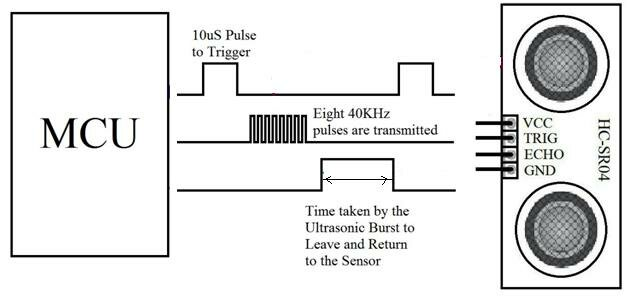
\includegraphics[width=0.70\textwidth]{exp2_hcsr04_pin.jpg}
    \caption{แผนผังขาเชื่อมต่อ (Pin Diagram) ของเซนเซอร์ HC-SR04}
    \label{fig:hcsr04_pin}
\end{figure}

\paragraph{Timing Diagram และลำดับการทำงาน}

หลักการทำงานของ HC-SR04 แบ่งออกเป็น 3 ช่วงหลัก

\begin{enumerate}
    \item \textbf{การสั่งงาน (Trigger Input):} ไมโครคอนโทรลเลอร์ส่งสัญญาณพัลส์
          HIGH ไปที่ขา TRIG เป็นเวลาอย่างน้อย $10\,\mu$s
    \item \textbf{การส่งคลื่น (Sonic Burst):} เซนเซอร์สร้างคลื่นอัลตราโซนิค
          ความถี่ 40~kHz จำนวน 8 ไซเคิล และยิงออกไปในอากาศ
    \item \textbf{การสะท้อนและอ่านค่า (Echo Pulse):} ขา ECHO
          เปลี่ยนสถานะจาก LOW เป็น HIGH ทันทีที่ส่งคลื่นเสร็จ
          และกลับมาเป็น LOW เมื่อรับสัญญาณสะท้อนกลับมาได้
\end{enumerate}

\textit{ข้อควรระวัง:} ต้องเว้นระยะห่างระหว่างรอบการวัดอย่างน้อย 60~ms
เพื่อป้องกันคลื่นสะท้อนตกค้างจากรอบก่อนหน้า

\begin{figure}[htbp]
    \centering
    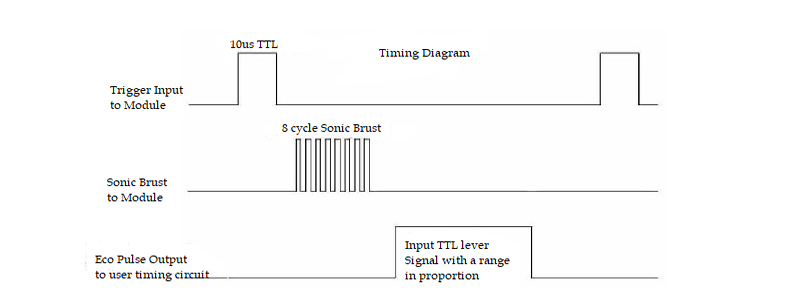
\includegraphics[width=0.90\textwidth]{exp2_hcsr04_timing.png}
    \caption{Timing Diagram ของ HC-SR04 แสดงลำดับสัญญาณ Trigger,
             Sonic Burst, และ Echo Pulse}
    \label{fig:hcsr04_timing}
\end{figure}

\paragraph{การคำนวณระยะทางจากพัลส์ Echo}

ที่อุณหภูมิห้องประมาณ 20°C ความเร็วของเสียงในอากาศมีค่าเท่ากับ 343.4~m/s
หรือ 0.0343~cm/$\mu$s เนื่องจากเวลา $T$ ที่วัดได้คือเวลาเดินทางแบบไป-กลับ
ระยะทางจริงจึงต้องหารด้วย 2 ดังนี้

\begin{equation}
    s = \frac{v_{\mathrm{sound}} \times T}{2}
      = \frac{0.0343\,[\mathrm{cm/\mu s}] \times T\,[\mu\mathrm{s}]}{2}
      = \frac{T}{58.31}
      \approx \frac{T}{58} \; \text{(cm)}
    \label{eq:hcsr04_derived}
\end{equation}

การปัดค่า 58.31 เป็น 58 เป็นการประมาณเพื่อลดภาระการคำนวณใน
ไมโครคอนโทรลเลอร์

%% ──────────────────────────────────────────────────────────────────
\subsubsection{การ Configure STM32 Nucleo G474RE สำหรับ HC-SR04}

การอ่านค่าจาก HC-SR04 บน STM32 Nucleo G474RE ต้องการการตั้งค่าฮาร์ดแวร์
สองส่วนหลัก

\begin{itemize}
    \item \textbf{GPIO Configuration:} ขา TRIG ตั้งเป็น GPIO Output Push-Pull
          สำหรับส่งพัลส์ $10\,\mu$s และขา ECHO ตั้งเป็น GPIO Input
          สำหรับรับสัญญาณ
    \item \textbf{Timer Configuration (TIM1):} ใช้เป็น Free-Running Counter
          ที่ความละเอียด $1\,\mu$s/count โดยตั้ง Prescaler = 169
          จาก System Clock 170~MHz ทำให้ Timer นับที่ 1~MHz พอดี
          สามารถวัดความกว้างพัลส์ Echo ได้โดยตรงในหน่วย microseconds
\end{itemize}

\begin{table}[htbp]
    \centering
    \caption{การเชื่อมต่อ HC-SR04 กับ STM32 Nucleo G474RE}
    \label{tab:hcsr04_wiring}
    \begin{tabular}{llp{6cm}}
        \hline
        \textbf{HC-SR04 Pin} & \textbf{Nucleo G474RE Pin} & \textbf{หน้าที่} \\
        \hline
        VCC  & 5V        & ไฟเลี้ยง \\
        GND  & GND       & กราวด์ \\
        TRIG & PA9 (D8)  & GPIO Output --- ส่งพัลส์ $10\,\mu$s \\
        ECHO & PA8 (D7)  & GPIO Input --- รับพัลส์วัดระยะ \\
        \hline
    \end{tabular}
\end{table}

%% ──────────────────────────────────────────────────────────────────
\subsubsection{การคำนวณ Sample Variance เพื่อหาค่า $R$}

ค่า Measurement Noise Covariance $R$ ของ Kalman Filter คือ Variance
ของ Noise ของเซนเซอร์ ซึ่งประมาณได้จาก Sample Variance ของ Raw Data
ที่เก็บขณะวัตถุอยู่นิ่ง ดังสมการ

\begin{equation}
    s^2 = \frac{\displaystyle\sum_{i=1}^{N}(z_i - \bar{z})^2}{N - 1}
    \label{eq:exp2_sample_variance}
\end{equation}

โดยที่ $z_i$ คือค่าที่อ่านได้จากเซนเซอร์แต่ละครั้ง $\bar{z}$ คือค่าเฉลี่ย
และ $N$ คือจำนวนตัวอย่าง การหารด้วย $N-1$ แทน $N$ เรียกว่า
Bessel's Correction เพื่อให้ Sample Variance เป็น Unbiased Estimator
ของ Population Variance ที่แท้จริง

เมื่อมีการทำซ้ำหลาย Trials ค่า $R$ ที่ใช้จริงคือค่าเฉลี่ยของ
Sample Variance ข้าม $M$ Trials

\begin{equation}
    R = \bar{s}^2 = \frac{1}{M} \sum_{j=1}^{M} s_j^2
    \label{eq:exp2_mean_variance}
\end{equation}

โดยที่ $s_j^2$ คือ Sample Variance ของ Trial ที่ $j$
และ $M$ คือจำนวน Trials ทั้งหมด

\subsubsection{Kalman Filter ใน Continuous Domain}

ก่อนที่จะนำ Kalman Filter ไปใช้งานบนไมโครคอนโทรลเลอร์ในรูปแบบ Discrete
จำเป็นต้องเข้าใจรูปแบบ Continuous Domain ก่อน
Kalman--Bucy Filter คือรูปแบบ Continuous ของ Kalman Filter
ซึ่งประมาณค่าสถานะของระบบ LTI ที่อธิบายด้วยสมการ

\begin{align}
    \dot{x}(t) &= Ax(t) + Bu(t) + w(t) \label{eq:ct_state} \\
    z(t)        &= Hx(t) + v(t)          \label{eq:ct_obs}
\end{align}

โดยที่ $w(t) \sim \mathcal{N}(0, Q_c)$ คือ Process Noise
และ $v(t) \sim \mathcal{N}(0, R)$ คือ Measurement Noise
สมการ Kalman--Bucy Filter ใน Continuous Domain มีรูปแบบ

\begin{equation}
    \dot{\hat{x}}(t) = A\hat{x}(t) + Bu(t) + K_f(t)\bigl(z(t) - H\hat{x}(t)\bigr)
    \label{eq:kalman_bucy}
\end{equation}

โดยที่ $K_f(t) = P(t)H^TR^{-1}$ คือ Kalman Gain แบบ Continuous
และ $P(t)$ คือ Error Covariance 

\begin{equation}
    \dot{P}(t) = AP(t) + P(t)A^T + Q_c - P(t)H^TR^{-1}HP(t)
    \label{eq:riccati}
\end{equation}

อย่างไรก็ตาม การ Implement สมการเหล่านี้บนไมโครคอนโทรลเลอร์โดยตรงไม่สามารถ
ทำได้ เนื่องจากระบบฝังตัวทำงานในเวลาแบบ Discrete จึงต้องทำการ Discretize
สมการก่อนนำไปใช้งาน ดังที่จะอธิบายในหัวข้อถัดไป

\subsubsection{การ Discretize สมการ Kalman Filter}

การแปลงสมการ Kalman Filter จาก Continuous Domain ไปเป็น Discrete Domain
ทำได้โดยใช้วิธี Zero-Order Hold (ZOH) หรือ Euler Forward
สำหรับ Scalar KF ที่ใช้กับ HC-SR04 ในการทดลองนี้
กำหนดพารามิเตอร์ของระบบดังนี้

\begin{itemize}
    \item ระบบมีสถานะเดียวคือระยะทาง $x_k$ (Scalar)
    \item ไม่มี Control Input ดังนั้น $B = 0$
    \item Sensor วัดสถานะได้โดยตรง ดังนั้น $H = 1$
    \item ระบบสมมติให้สถานะไม่เปลี่ยนแปลงระหว่าง Step
    ดังนั้น $A_c = 0$ ซึ่งนำไปสู่ $F = e^{A_c T_s} = 1$
\end{itemize}

เมื่อใช้ Euler Forward Approximation $F \approx I + A_c T_s$
และ $A_c = 0$ สำหรับระบบ Static Model จะได้

กระบวนการ Discretize เริ่มจาก Continuous-Domain State Equation:

\begin{equation}
    \dot{x}(t) = A_c\,x(t) + B_c\,u(t) + w(t)
    = 0 \cdot x(t) + 0 \cdot u(t) + w(t)
    \label{eq:scalar_continuous}
\end{equation}

ซึ่งสะท้อนว่าในแบบจำลอง Static Model สถานะจริงไม่มี
แนวโน้มเปลี่ยนแปลงเอง ความเปลี่ยนแปลงที่เกิดขึ้นถูกจำลอง
ผ่าน Process Noise $w(t)$ เท่านั้น

จากนั้นใช้ Zero-Order Hold (ZOH) เพื่อแปลง $A_c$ ไปเป็น
Discrete State Transition Matrix $F$:

\begin{equation}
    F = e^{A_c T_s}
      = e^{0 \cdot T_s}
      = e^{0}
      = 1
    \label{eq:scalar_F_derive}
\end{equation}

และ Discrete Input Matrix:

\begin{equation}
    B_d = \int_0^{T_s} e^{A_c \tau}\,B_c\,d\tau
        = \int_0^{T_s} 1 \cdot 0\,d\tau
        = 0
    \label{eq:scalar_Bd_derive}
\end{equation}

ผลลัพธ์ที่ได้คือ Discrete State-Space Model สำหรับ Scalar KF:

\begin{align}
    x_k      &= F\,x_{k-1} + B_d\,u_{k-1} + w_{k-1}
               = x_{k-1} + w_{k-1}
               \label{eq:scalar_state_disc} \\
    z_k      &= H\,x_k + v_k
               = x_k + v_k
               \label{eq:scalar_obs_disc}
\end{align}

ซึ่งสอดคล้องกับสมมติฐานที่ว่าระยะทางที่แท้จริงไม่เปลี่ยนแปลง
ระหว่าง Sampling Period และ Sensor วัดสถานะได้โดยตรงแต่มี Noise

%% ─────────────────────────────────────────
\subsubsection{สรุปสมการคณิตศาสตร์ของ Discrete Kalman Filter}

ก่อนที่จะนำอัลกอริทึมไปเขียนเป็นโปรแกรมลงบนไมโครคอนโทรลเลอร์ STM32 ขอสรุปสมการหลักทั้ง 5 ขั้นตอนของ Discrete Kalman Filter ซึ่งแบ่งการทำงานออกเป็น 2 ระยะ (Phase) อย่างเป็นวงรอบ (Recursive) ได้แก่ ระยะพยากรณ์ (Prediction Step) และระยะปรับปรุง (Update Step) ดังนี้



\textbf{1. ระยะพยากรณ์ (Prediction Step / Time Update)}
ขั้นตอนนี้ทำหน้าที่คาดการณ์สถานะล่วงหน้าหนึ่งสเต็ปเวลา โดยอาศัยแบบจำลองทางคณิตศาสตร์ (State-Space Model) ของระบบ
\begin{align}
    \hat{x}_{k|k-1} &= A \hat{x}_{k-1|k-1} + B u_k \label{eq:kf_predict_state} \\
    P_{k|k-1} &= A P_{k-1|k-1} A^T + Q \label{eq:kf_predict_cov}
\end{align}

\textbf{2. ระยะปรับปรุง (Update Step / Measurement Update)}
ขั้นตอนนี้ทำหน้าที่นำข้อมูลจริงที่วัดได้จากเซนเซอร์ ณ เวลานั้น มาปรับแก้ค่าที่พยากรณ์ไว้ให้มีความแม่นยำยิ่งขึ้น โดยให้น้ำหนักความเชื่อถือผ่านค่า Kalman Gain
\begin{align}
    K_k &= P_{k|k-1} H^T (H P_{k|k-1} H^T + R)^{-1} \label{eq:kf_kalman_gain} \\
    \hat{x}_{k|k} &= \hat{x}_{k|k-1} + K_k (z_k - H \hat{x}_{k|k-1}) \label{eq:kf_update_state} \\
    P_{k|k} &= (I - K_k H) P_{k|k-1} \label{eq:kf_update_cov}
\end{align}

รายละเอียดของตัวแปรในสมการมีดังนี้:
\begin{itemize}
    \item $\hat{x}$: สถานะของระบบ (State Estimate) เช่น ตำแหน่ง หรือ ความเร็ว
    \item $P$: ความแปรปรวนร่วมของความคลาดเคลื่อน (Error Covariance) สะท้อนถึงความไม่แน่นอนของการประมาณค่า
    \item $A, B, H$: เมทริกซ์พลวัตของระบบ (System Dynamics), เมทริกซ์อินพุต (Input Matrix), และเมทริกซ์สังเกตการณ์ (Measurement Matrix)
    \item $Q, R$: ค่าความแปรปรวนของสัญญาณรบกวนในกระบวนการ (Process Noise Covariance) และจากการวัด (Measurement Noise Covariance)
    \item $K_k$: อัตราขยายคาลมาน (Kalman Gain) ซึ่งเป็นตัวกำหนดน้ำหนักระหว่างแบบจำลองกับเซนเซอร์
    \item $z_k$: ค่าที่อ่านได้จริงจากเซนเซอร์ (Measurement)
\end{itemize}

\textit{หมายเหตุ:} สำหรับระบบแบบ Scalar (1 มิติ) เมทริกซ์ทั้งหมดจะลดรูปลงเป็นค่าคงที่ (Scalar value) การดำเนินการทรานสโพส ($^T$) จะไม่มีผล และการอินเวอร์สเมทริกซ์ ($^{-1}$) จะถูกแทนที่ด้วยการหารทางคณิตศาสตร์ทั่วไป

โค้ดด้านล่างแสดงการ Implement Scalar KF ในภาษา C บนไมโครคอนโทรลเลอร์ STM32 Nucleo G474RE โดยแต่ละขั้นตอนสอดคล้องกับสมการ~\eqref{eq:kf_predict_state}--\eqref{eq:kf_update_cov} อย่างสมบูรณ์

\subsubsection{การ Implement Scalar Kalman Filter บน STM32}

โค้ดด้านล่างแสดงการ Implement Scalar KF ใน C บน STM32 Nucleo G474RE
โดยแต่ละขั้นตอนสอดคล้องกับสมการ~\eqref{eq:kf_predict_state}--\eqref{eq:kf_update_cov}

\begin{lstlisting}[language=C, caption={Scalar Kalman Filter — kalman.c},
                   label={lst:scalar_kf}]
typedef struct {
    float x_est;   // Estimated state
    float P;       // Error covariance
    float Q;       // Process noise covariance
    float R;       // Measurement noise covariance
} KalmanScalar_t;

void Kalman_Init(KalmanScalar_t *kf, float Q, float R, float x0)
{
    kf->x_est = x0;
    kf->P     = 1.0f;
    kf->Q     = Q;
    kf->R     = R;
}

float Kalman_Update(KalmanScalar_t *kf, float z)
{
    // Prediction
    float x_prior = kf->x_est;
    float P_prior = kf->P + kf->Q;

    // Update
    float K = P_prior / (P_prior + kf->R);
    kf->x_est = x_prior + K * (z - x_prior);
    kf->P = (1.0f - K) * P_prior;

    return kf->x_est;
}
\end{lstlisting}

\noindent ใน Main Loop การใช้งาน Filter มีโครงสร้างดังนี้

\begin{lstlisting}[language=C, caption={main.c — Main Loop สำหรับ Scalar KF},
                   label={lst:main_kf}]
KalmanScalar_t kf;
float raw_cm, filtered_cm;

HAL_TIM_Base_Start(&htim1);
HCSR04_Init(&htim1);
raw_cm = HCSR04_Read();

Kalman_Init(&kf, Q_VALUE, R_VALUE, raw_cm);

while (1) {
    raw_cm = HCSR04_Read();

    if (raw_cm > 0.0f) {
        filtered_cm = Kalman_Update(&kf, raw_cm);
        printf("%lu,%.4f,%.4f\r\n", HAL_GetTick(), raw_cm, filtered_cm);
        fflush(stdout);
    }
    HAL_Delay(60);
}
\end{lstlisting}

%% ─────────────────────────────────────────────────────────────────────────────
\subsection{ขั้นตอนการทดลอง}

\begin{enumerate}
    \item พัฒนา Library \texttt{hcsr04.c} สำหรับเชื่อมต่อ HC-SR04
          กับ Nucleo G474RE โดยใช้ Timer TIM1 ที่ความละเอียด $1\,\mu$s
          และประมวลผลระยะทางเป็นชนิดข้อมูล \texttt{float}
    \item ต่อสาย HC-SR04 กับ Nucleo G474RE ตามตารางที่~\ref{tab:hcsr04_wiring}
    \item ส่งข้อมูลระยะทางดิบผ่าน LPUART1 (Baud rate 115200)
          ออกมาที่คอมพิวเตอร์เป็น CSV format
    \item วางวัตถุแบนตั้งฉากกับเซนเซอร์ที่ระยะเป้าหมาย 10~cm แล้วบันทึก
          500 ตัวอย่าง ทำซ้ำ 5 Trials โดยในแต่ละ Trial ปล่อยให้ระบบ
          นิ่งก่อนเริ่มบันทึกข้อมูล
    \item ทำซ้ำข้อ 4 ที่ระยะ 20~cm และ 30~cm
    \item นำข้อมูลเข้า MATLAB คำนวณ Sample Variance ของแต่ละ Trial
          ตามสมการ~\eqref{eq:exp2_sample_variance} และหาค่าเฉลี่ย
          ตามสมการ~\eqref{eq:exp2_mean_variance}
    \item เลือกค่า $R$ ที่สอดคล้องกับ Operating Range ของระบบ
          Mass-Spring-Damper
\end{enumerate}

%% ─────────────────────────────────────────────────────────────────────────────
\subsection{การพัฒนา Library HC-SR04}

\subsubsection{โครงสร้าง Library (\texttt{hcsr04.h} / \texttt{hcsr04.c})}

Library ประกอบด้วยสองฟังก์ชันหลัก ได้แก่
\texttt{HCSR04\_Init()} สำหรับตั้งค่า Timer และ GPIO
และ \texttt{HCSR04\_Read()} สำหรับวัดระยะจริง
โดยกำหนดค่าคงที่ไว้ใน \texttt{hcsr04.h}

\begin{lstlisting}[language=C,
    caption={\texttt{hcsr04.h} --- ค่าคงที่และ Function Prototype},
    label={lst:hcsr04_h}]
#define HCSR04_TRIG_PIN              GPIO_PIN_9
#define HCSR04_TRIG_PORT             GPIOA

#define HCSR04_ECHO_PIN              GPIO_PIN_8
#define HCSR04_ECHO_PORT             GPIOA

#define HCSR04_ECHO_HIGH_TIMEOUT_MS  30U
#define HCSR04_ECHO_LOW_TIMEOUT_MS   50U
#define HCSR04_TIMEOUT_VALUE         -1.0f
#define HCSR04_MIN_INTERVAL_MS       60U

void  HCSR04_Init(TIM_HandleTypeDef *htim);
float HCSR04_Read(void);
\end{lstlisting}

\subsubsection{การทำงานของ \texttt{HCSR04\_Read()}}

ฟังก์ชัน \texttt{HCSR04\_Read()} คืนค่าระยะทางในหน่วย cm แบบ \texttt{float}
มีขั้นตอนการทำงานดังนี้

\begin{lstlisting}[language=C,
    caption={\texttt{hcsr04.c} --- การวัดระยะของ \texttt{HCSR04\_Read()}},
    label={lst:hcsr04_read}]
float HCSR04_Read(void) {
    uint32_t v1, v2, t_start;

    // Trigger pulse
    HAL_GPIO_WritePin(HCSR04_TRIG_PORT, HCSR04_TRIG_PIN, GPIO_PIN_SET);
    __HAL_TIM_SET_COUNTER(hcsr04_htim, 0);
    while (__HAL_TIM_GET_COUNTER(hcsr04_htim) < 10);
    HAL_GPIO_WritePin(HCSR04_TRIG_PORT, HCSR04_TRIG_PIN, GPIO_PIN_RESET);

    // Wait for Echo rising edge
    __HAL_TIM_SET_COUNTER(hcsr04_htim, 0);
    t_start = HAL_GetTick();
    while (HAL_GPIO_ReadPin(HCSR04_ECHO_PORT, HCSR04_ECHO_PIN) == GPIO_PIN_RESET) {
        if ((HAL_GetTick() - t_start) >= HCSR04_ECHO_HIGH_TIMEOUT_MS) return -1.0f;
    }
    v1 = __HAL_TIM_GET_COUNTER(hcsr04_htim);

    // Wait for Echo falling edge
    t_start = HAL_GetTick();
    while (HAL_GPIO_ReadPin(HCSR04_ECHO_PORT, HCSR04_ECHO_PIN) == GPIO_PIN_SET) {
        if ((HAL_GetTick() - t_start) >= HCSR04_ECHO_LOW_TIMEOUT_MS) return -1.0f;
    }
    v2 = __HAL_TIM_GET_COUNTER(hcsr04_htim);

    return (float)(v2 - v1) / 58.0f; // Convert to cm
}
\end{lstlisting}

\subsubsection{Main Loop สำหรับเก็บข้อมูล Raw Data}

Main loop ที่ใช้ในการเก็บข้อมูล Raw Data เพื่อคำนวณ Variance
มีโครงสร้างดังนี้

\begin{lstlisting}[language=C,
    caption={\texttt{main.c} --- Main Loop สำหรับส่ง Raw Distance ออก Serial},
    label={lst:main_raw}]
HAL_TIM_Base_Start(&htim1);
HCSR04_Init(&htim1);

while (1) {
    float raw_cm = HCSR04_Read();

    if (raw_cm > 0.0f) {
        printf("%lu,%.4f\r\n", HAL_GetTick(), raw_cm);
        fflush(stdout);
    }
    HAL_Delay(60);
}
\end{lstlisting}

%% ─────────────────────────────────────────────────────────────────────────────
\subsection{ผลการทดลอง}

\subsubsection{ผลการประเมินค่า Measurement Noise Covariance ($R$)}

จากการเก็บข้อมูล 5 Trials, 500 Samples ต่อ Trial ที่ระยะเป้าหมาย
10, 20, และ 30~cm แล้วคำนวณ Sample Variance ของแต่ละ Trial
และหาค่าเฉลี่ยตามสมการ~\eqref{eq:exp2_mean_variance}
ผลลัพธ์สรุปได้ดังตารางที่~\ref{tab:variance_results}

\begin{table}[htbp]
    \centering
    \caption{ผลการประมวลผล Variance เฉลี่ยจาก 5 Trials,
             500 Samples ต่อ Trial}
    \label{tab:variance_results}
    \begin{tabular}{cccc}
        \hline
        \textbf{ระยะ (cm)}
            & \textbf{ค่าเฉลี่ย $\bar{z}$ (cm)}
            & \textbf{$R = \bar{s}^2$ (cm$^2$)}\\
        \hline
        10 & 9.297  & 0.0050\\
        20 & 18.847 & 0.0337\\
        30 & 28.954 & 0.0734\\
        \hline
    \end{tabular}
\end{table}

จากตารางที่~\ref{tab:variance_results} พบว่าเมื่อระยะห่างของเป้าหมายเพิ่มขึ้น
ความแปรปรวนของสัญญาณก็จะเพิ่มขึ้นตามไปด้วยอย่างชัดเจน

\begin{figure}[htbp]
    \centering
    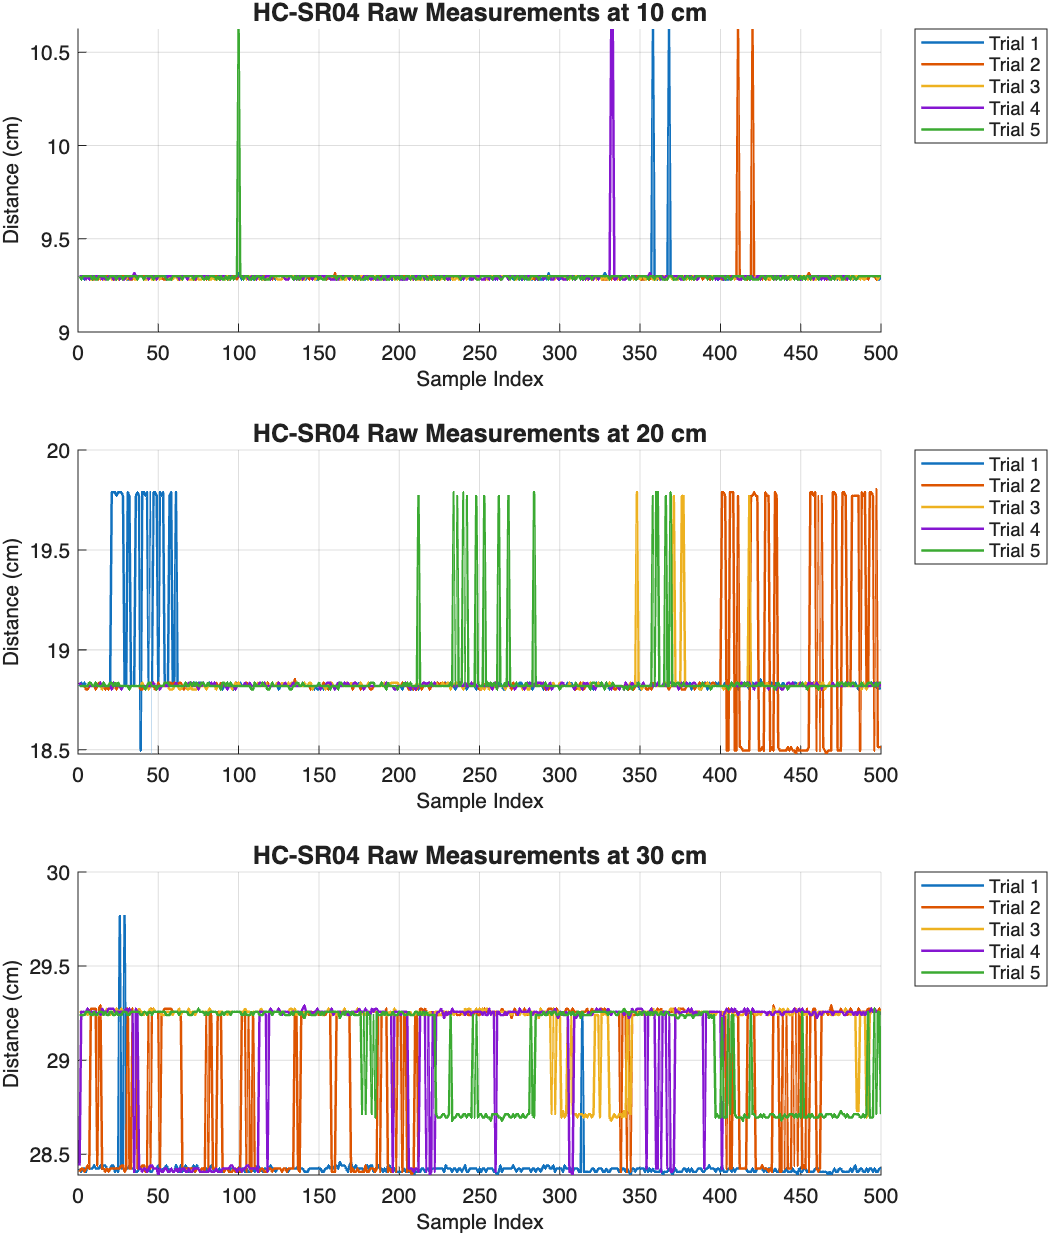
\includegraphics[width=0.85\textwidth]{exp2_variance_plot.png}
    \caption{กราฟแสดงข้อมูลดิบ (Raw Data) จาก 5 Trials ที่ระยะ 10, 20, และ 30~cm
             แต่ละ Trial บันทึก 500 Samples เพื่อเปรียบเทียบความแตกต่างของ Variance
             ในแต่ละระยะ}
    \label{fig:exp2_variance_plot}
\end{figure}

\subsubsection{การเลือกค่า $R$ สำหรับระบบ Mass-Spring-Damper}

ระบบ Mass-Spring-Damper ในการทดลองถัดไปมีขอบเขตการเคลื่อนที่
สูงสุดประมาณ 20~cm จึงเลือกใช้ $R = 0.0337~\text{cm}^2$
จากระยะ 20~cm เป็นค่าอ้างอิงสำหรับ Kalman Filter ในการทดลองที่ 3 และ 5

% \subsubsection{ขั้นตอนการเลือกค่า \texorpdfstring{$Q$}{Q} สำหรับ Scalar KF}

% การเลือกค่า Process Noise Covariance $Q$ ดำเนินการตามขั้นตอนดังนี้

% \textbf{ขั้นที่ 1 — กำหนดขอบเขตบนและล่างของ $Q$ จากค่า $R$}

% เนื่องจาก $Q$ และ $R$ ควบคุมอัตราส่วนความเชื่อมั่นระหว่าง Model
% และ Sensor ร่วมกัน จึงใช้ $R$ เป็นจุดอ้างอิง:

% \begin{itemize}
%     \item หาก $Q \gg R$: Filter เชื่อ Measurement เกือบทั้งหมด
%           สัญญาณออกจะ Noisy ใกล้เคียง Raw Data
%     \item หาก $Q \ll R$: Filter เชื่อ Model เกือบทั้งหมด
%           สัญญาณออกจะเรียบมากแต่ตอบสนองช้า
%     \item ช่วงที่น่าสนใจจึงอยู่ระหว่าง $Q \approx 10^{-6}$
%           ถึง $Q \approx 10^{-3}$ ซึ่งครอบคลุมทั้งสองด้าน
% \end{itemize}

% \textbf{ขั้นที่ 2 — เลือกค่าเริ่มต้นโดยอ้างอิงจาก Variance ของ Sensor}

% จากการทดลองวัด Variance ของ HC-SR04 ที่ระยะใกล้ (10 cm) ได้
% $s^2 = 0.0050$ cm$^2$ ซึ่งสะท้อนระดับ Noise พื้นฐานที่ต่ำที่สุด
% ในระบบ จึงเลือก $Q = 1 \times 10^{-5}$ เป็นค่า Nominal เนื่องจาก:

% \begin{equation}
%     Q_\text{nominal} = 1 \times 10^{-5}
%     \approx \frac{1}{500} \times R
%     = \frac{1}{500} \times 0.0337
%     \label{eq:Q_nominal_ratio}
% \end{equation}

% ซึ่งทำให้ $Q/R \approx 3 \times 10^{-4}$ กล่าวคือ Filter โน้มเอียง
% ไปทาง Model เป็น Default อันสอดคล้องกับ Static Sensor System
% ที่คาดว่าระยะทางจริงเปลี่ยนแปลงน้อยมากระหว่าง Sampling Period

% \textbf{ขั้นที่ 3 — ตรวจสอบพฤติกรรมจากกราฟ}

% นำค่า $Q_\text{nominal}$ ไปรันกับข้อมูลจริงแล้วสังเกต:

% \begin{itemize}
%     \item สัญญาณออก $\hat{x}_k$ เรียบกว่า Raw Data อย่างเห็นได้ชัด
%           และไม่มี Lag ที่รับรู้ได้ในสภาวะ Static
%     \item เมื่อระยะทางเปลี่ยนแบบ Step Change
%           Filter สามารถติดตามได้ภายในเวลาที่ยอมรับได้
% \end{itemize}

% ผลการทดสอบพบว่า $Q = 1 \times 10^{-5}$ ให้สมดุลที่ดีที่สุด
% ระหว่าง Smoothness และ Responsiveness สำหรับ Application นี้
% สอดคล้องกับค่า Nominal ที่ Al Tahtawi (2018) เลือกใช้เช่นกัน
% ค่า $Q$ ทั้งสามระดับที่ทดสอบในการทดลองที่ 3 จึงเลือกรอบ
% ค่า Nominal นี้ คือ $Q \in \{1\times10^{-3},\,1\times10^{-5},\,1\times10^{-6}\}$

%% ─────────────────────────────────────────────────────────────────────────────
\subsection{สรุปผลการทดลอง}

\begin{itemize}
    \item สามารถพัฒนา Library \texttt{hcsr04.c}/\texttt{hcsr04.h}
          สำหรับอ่านค่าระยะทางจาก HC-SR04 บน STM32G4 ได้สำเร็จ
          โดยใช้ TIM1 เป็น Counter ความละเอียด $1\,\mu$s
          และมีระบบ Timeout เพื่อป้องกันการค้างของโปรแกรม
    \item จากการวัด 5 Trials, 500 Samples ต่อ Trial พบว่า Variance
          ของ HC-SR04 เพิ่มขึ้นตามระยะ: 0.0050~cm$^2$ ที่ 10~cm,
          0.0337~cm$^2$ ที่ 20~cm, และ 0.0734~cm$^2$ ที่ 30~cm
    \item เลือกใช้ $R = 0.0337~\text{cm}^2$ ซึ่งสอดคล้องกับ
          Operating Range ของระบบ Mass-Spring-Damper
          เพื่อนำไปใช้เป็นพารามิเตอร์ใน Kalman Filter ต่อไป
\end{itemize}

%% ─────────────────────────────────────────────────────────────────────────────
\subsection{อภิปรายผล}

\begin{itemize}
    \item \textbf{ปรากฏการณ์การขยายตัวของ Variance ตามระยะทาง:}
          Variance ที่เพิ่มขึ้นจาก 0.0050 ถึง 0.0734~cm$^2$ เป็นผลจาก
          Beam Divergence ของคลื่นอัลตราโซนิค เมื่อเป้าหมายอยู่ไกลขึ้น
          พลังงานคลื่นสะท้อนกลับลดลงและรับสัญญาณรบกวนสิ่งแวดล้อมได้มากขึ้น

    \item \textbf{Systematic Bias ของเซนเซอร์:}
          จากตารางที่~\ref{tab:variance_results} ค่าเฉลี่ยที่วัดได้มีความเบี่ยงเบน
          จากระยะจริง เช่น ที่ระยะ 10~cm วัดได้ 9.297~cm (ต่างจากจริง 0.703~cm)
          ซึ่งเป็น Systematic Error จากการวาง Reference และลักษณะเฉพาะของ Sensor
          ค่า Kalman Filter จะ Converge ไปยังค่าเฉลี่ยนี้ ไม่ใช่ค่าระยะจริง
          จึงต้องคำนึงถึงเมื่อนำไปประยุกต์ใช้

    \item \textbf{ความเหมาะสมในการเลือก $R = 0.0337~\text{cm}^2$:}
          หากใช้ $R$ จากระยะ 30~cm ($= 0.0734~\text{cm}^2$)
          ตัวกรองจะมีความเฉื่อยมากเกินไป ทำให้ตอบสนองช้า
          และหากใช้จาก 10~cm ($= 0.0050~\text{cm}^2$)
          ตัวกรองจะ Noisy มากเกินไป การใช้ค่าจาก 20~cm
          ซึ่งตรงกับ Operating Range จริงจึงเป็น Engineering Tradeoff
          ที่สมเหตุสมผลที่สุด

    \item \textbf{ความน่าเชื่อถือของผล:}
          การวัดซ้ำ 5 Trials ช่วยให้สามารถคำนวณค่า S.D. ของ Variance ข้าม Trials
          เพื่อยืนยัน Reproducibility ของการวัด ค่า S.D. ที่ต่ำแสดงว่า
          Noise Characteristic ของ Sensor มีความสม่ำเสมอและสามารถ
          ใช้เป็นพารามิเตอร์ที่เชื่อถือได้สำหรับ Kalman Filter
\end{itemize}
% !TeX root = ../main.tex

\section{การทดลองที่ 3: ผลกระทบของ $Q$ และอัตราส่วน $Q/R$
         ต่อพฤติกรรมของ Scalar KF}
% \textit{ครอบคลุม Criteria: Part 2 --- ออกแบบการทดลองแสดงผลของการปรับ $Q$,
% อธิบาย $Q/R$ Trade-off, เลือก Visualization ที่เหมาะสม (รวม 2.5 คะแนน)}

%% ─────────────────────────────────────────────────────────────────────────────
\subsection{บทนำ}

จากการทดลองที่ 2 ได้ Scalar Kalman Filter ที่ทำงานได้แล้ว พร้อมค่า
Measurement Noise Covariance $R = 0.0337\ \text{cm}^2$ ที่คำนวณได้จาก Variance
ของ Raw Data จริง อย่างไรก็ตาม การเลือกค่า $Q$ เป็นหนึ่งในการตัดสินใจทางวิศวกรรม
ที่สำคัญที่สุดในการออกแบบ Kalman Filter เนื่องจาก $Q$ ควบคุมสมดุลระหว่างสองเป้าหมาย
ที่ขัดแย้งกัน ได้แก่ \textbf{Smoothness} (ความเรียบของสัญญาณออก)
และ \textbf{Responsiveness} (ความไวในการติดตามการเปลี่ยนแปลง)

กลไกหลักที่ $Q$ ส่งผลผ่านคือสมการ Covariance Prediction:
\begin{equation}
    P_k^{(-)} = P_{k-1} + Q
    \label{eq:cov_predict_exp3}
\end{equation}
ทุกรอบที่ระบบทำงาน $Q$ จะ``ฉีด''ความไม่แน่นอนเข้าไปใน $P_k^{(-)}$
ทำให้ Kalman Gain $K_k$ มีค่าสูงขึ้น และ Filter หันมาเชื่อถือ Measurement มากขึ้น
ในทางกลับกัน $Q$ ที่ต่ำมากจะทำให้ $P_k^{(-)}$ ลู่เข้าศูนย์
ส่งผลให้ Filter หยุดรับข้อมูลใหม่จาก Sensor

การเลือกทดสอบ $Q \in \{1\times10^{-3},\ 1\times10^{-5},\ 1\times10^{-6}\}$
ตามแนวทางของ Al~Tahtawi (2018) เนื่องจากช่วงนี้ครอบคลุมอัตราส่วน $Q/R$
ตั้งแต่ระดับที่ Filter เชื่อ Measurement มากกว่า Model ($Q \gg R$)
ไปจนถึงระดับที่ Filter เชื่อ Model มากกว่า Measurement ($Q \ll R$)
ทำให้สามารถสังเกตพฤติกรรมสุดโต่งทั้งสองด้านได้ในการทดลองเดียวกัน
โดยใช้ $Q = 1\times10^{-5}$ เป็น Nominal Value เนื่องจากมีขนาดใกล้เคียงกับ
Variance ของ Raw Data ที่ระยะใกล้ ($s^2 = 0.0050\ \text{cm}^2$ ที่ระยะ 10 cm)
ซึ่งสะท้อนระดับความไม่แน่นอนของ Model ที่สมเหตุสมผลสำหรับ Sensor นี้

งานวิจัย Al~Tahtawi (2018) ได้ทดสอบค่า $Q$ สามระดับดังกล่าวบน HC-SR04
และพบว่า Output Noise Variance มีความสัมพันธ์แบบ Exponential กับขนาดของ $Q$
การทดลองนี้จึงทำซ้ำการทดสอบดังกล่าวบนแพลตฟอร์ม STM32 Nucleo G474RE
เพื่อยืนยันผลและเลือกค่า $Q$ ที่เหมาะสมที่สุดสำหรับการนำไปใช้จริง

%% ─────────────────────────────────────────────────────────────────────────────
\subsection{วัตถุประสงค์}

\begin{itemize}
    \item เพื่อศึกษาว่าการเปลี่ยนแปลงค่า $Q$ ส่งผลต่อพฤติกรรมของ KF อย่างไร
          ทั้งในสถานะคงที่ (Steady State) และเมื่อมี Step Change
    \item เพื่อทำความเข้าใจ Trade-off ระหว่าง Smoothness และ Responsiveness
          ที่ถูกควบคุมโดยอัตราส่วน $Q/R$
    \item เพื่อวัดผล Quantitative ของ Smoothness (Output Variance)
          และ Responsiveness (Response Time) สำหรับแต่ละ $Q$
    \item เพื่อเลือกและ Justify ค่า $Q$ ที่เหมาะสมที่สุดสำหรับ
          ระบบ HC-SR04 บน STM32 Nucleo G474RE
\end{itemize}

%% ─────────────────────────────────────────────────────────────────────────────
\subsection{สมมติฐาน}

\begin{itemize}
    \item $Q$ ที่มากขึ้นจะทำให้ Filter ตอบสนองเร็วขึ้น
          (ติดตาม Step Change ได้ไวขึ้น) แต่สัญญาณออกจะมี Noise มากขึ้น
    \item $Q$ ที่น้อยลงจะให้สัญญาณออกเรียบขึ้น
          แต่เกิด Lag Error เมื่อระยะทางจริงเปลี่ยนอย่างกะทันหัน
    \item Output Noise Variance จะมีความสัมพันธ์เป็นเชิงบวกกับขนาดของ $Q$
          ตามที่ Al Tahtawi (2018) รายงานไว้
    \item มีช่วงค่า $Q$ ที่ให้ผลสมดุลระหว่าง Smoothness และ Responsiveness
          สำหรับ Sensor และ Application นี้โดยเฉพาะ
\end{itemize}

%% ─────────────────────────────────────────────────────────────────────────────
\subsection{ตัวแปร}

\begin{itemize}
    \item \textbf{ตัวแปรอิสระ:} ค่า $Q$ ที่ทดสอบ 3 ระดับ
          ตาม Al Tahtawi (2018) ได้แก่
          $Q = 1\times10^{-3}$, $Q = 1\times10^{-5}$, และ $Q = 1\times10^{-6}$
    \item \textbf{ตัวแปรตาม:} Variance ของ KF Output (วัด Smoothness),
          Response Time หลัง Step Change (วัด Responsiveness),
          Steady-State Kalman Gain $K_{k,\mathrm{ss}}$
    \item \textbf{ตัวแปรควบคุม:} ค่า $R = 0.0337$~cm$^2$ คงที่
          (จากการทดลองที่ 2), Sampling Time $T_s = 60$~ms คงที่,
          Scenario การทดสอบเหมือนกันทุกค่า $Q$
\end{itemize}

%% ─────────────────────────────────────────────────────────────────────────────
\subsection{เอกสารและงานวิจัยที่เกี่ยวข้อง}

\subsubsection{ความหมายทางกายภาพของ Process Noise Covariance $Q$}

$Q$ คือพารามิเตอร์ที่สะท้อน \textbf{ความไม่เชื่อมั่นใน Dynamic Model} ของระบบ
หากระบบจริงมีพฤติกรรมที่ Model ไม่ได้จำลอง (เช่น การเคลื่อนที่ของเป้าหมายในระบบ Static
หรือแรงรบกวนที่ Model ไม่ครอบคลุม) $Q$ ควรมีค่าสูงขึ้นเพื่อให้ Filter
มีความยืดหยุ่นพอที่จะปรับตัวตามสถานการณ์จริง ในทางตรงข้าม
หากระบบจริงสอดคล้องกับ Model อย่างแม่นยำ $Q$ ควรมีค่าต่ำ

แนวคิดนี้แตกต่างจาก $R$ ซึ่งสะท้อนความไม่เชื่อมั่นใน \textbf{Sensor}
ความสัมพันธ์ระหว่าง $Q$ และ $R$ จึงกำหนดว่า Filter จะ ``เชื่อ Model''
หรือ ``เชื่อ Sensor'' มากกว่ากัน ซึ่งควบคุมโดยอัตราส่วน $Q/R$

\subsubsection{กลไกผ่านสมการ Covariance Prediction}

จากสมการ Covariance Prediction ของ Scalar KF
\begin{equation}
    P_k^{(-)} = P_{k-1} + Q
    \label{eq:cov_pred_detail}
\end{equation}

$Q$ บวกเข้าไปใน $P_k^{(-)}$ ทุกรอบ ทำให้ $P_k^{(-)}$ ไม่สามารถลู่เข้าศูนย์ได้
ผลที่ได้คือ Kalman Gain
\begin{equation}
    K_k = \frac{P_k^{(-)}}{P_k^{(-)} + R}
    \label{eq:scalar_gain_exp3}
\end{equation}
จะ Converge ไปสู่ค่า Steady-State $K_{k,\mathrm{ss}}$ ที่ไม่เป็นศูนย์
ค่า $K_{k,\mathrm{ss}}$ หาได้จากการแก้สมการกำลังสองของ $P_\mathrm{ss}$
\begin{equation}
    P_\mathrm{ss}^2 + Q \cdot P_\mathrm{ss} - Q \cdot R = 0
    \label{eq:p_ss_quadratic}
\end{equation}
ซึ่งมีรากบวกเป็น
\begin{equation}
    P_\mathrm{ss} = \frac{-Q + \sqrt{Q^2 + 4QR}}{2}
    \label{eq:p_ss_solution}
\end{equation}

ที่ค่า $R = 0.0337$~cm$^2$ ที่ได้จากการทดลองที่ 2
$K_{k,\mathrm{ss}}$ ของ $Q$ ทั้งสามค่ามีดังต่อไปนี้

\begin{table}[htbp]
    \centering
    \caption{ค่า Steady-State Kalman Gain สำหรับแต่ละ $Q$
             (คำนวณจากสมการ~\eqref{eq:p_ss_solution}, $R = 0.0337$~cm$^2$)}
    \label{tab:kss_theory}
    \begin{tabular}{cccc}
        \hline
        \textbf{ค่า $Q$} & \textbf{$Q/R$} & \textbf{$P_\mathrm{ss}$ (cm$^2$)} & \textbf{$K_{k,\mathrm{ss}}$} \\
        \hline
        $1\times10^{-3}$ & $2.97\times10^{-2}$ & $0.00533$ & $0.136$ \\
        $1\times10^{-5}$ & $2.97\times10^{-4}$ & $0.00058$ & $0.017$ \\
        $1\times10^{-6}$ & $2.97\times10^{-5}$ & $0.00018$ & $0.005$ \\
        \hline
    \end{tabular}
\end{table}

จากตารางที่~\ref{tab:kss_theory} จะเห็นได้ว่าทั้งสาม $Q$ มีอัตราส่วน $Q/R \ll 1$
เนื่องจาก $R = 0.0337$~cm$^2$ มีขนาดใหญ่กว่า $Q$ ทุกค่ามาก
การจัดอันดับของ $K_{k,\mathrm{ss}}$ และพฤติกรรมที่แตกต่างกันจึงมาจาก
\textbf{ขนาดสัมพัทธ์ระหว่าง $Q$ ด้วยกันเอง} ไม่ใช่จากความสัมพันธ์
$Q$ vs.\ $R$ โดยตรง

%% ─────────────────────────────────────────
\subsubsection{Trade-off ระหว่าง Smoothness และ Responsiveness}

หัวใจสำคัญของการออกแบบ Kalman Filter คือการหาจุดสมดุล (Trade-off) ระหว่างการกำจัดสัญญาณรบกวนให้ได้มากที่สุด (Smoothness) และการรักษาความสามารถในการติดตามการเปลี่ยนแปลงของสัญญาณจริงให้ได้เร็วที่สุด (Responsiveness) พฤติกรรมนี้ถูกควบคุมโดยตรงจากอัตราส่วน $Q/R$ ซึ่งเป็นตัวกำหนดค่าอัตราขยายคาลมานในสภาวะคงตัว (Steady-State Kalman Gain, $K_{k,ss}$) 

ตารางที่ \ref{tab:q_tradeoff} สรุปความสัมพันธ์ระหว่างพารามิเตอร์ที่ใช้ทดสอบกับผลลัพธ์เชิงคุณภาพที่สังเกตได้จากกราฟการทดลอง

\begin{table}[htbp]
    \centering
    \caption{สรุป Trade-off ของผลการตอบสนองในแต่ละระดับค่า $Q$}
    \label{tab:q_tradeoff}
    \begin{tabular}{ccccc}
        \hline
        \textbf{ค่า $Q$} & \textbf{อัตราส่วน $Q/R$} & \textbf{$K_{k,ss}$} & \textbf{Smoothness} & \textbf{Response Time} \\
        \hline
        $1 \times 10^{-3}$ & $2.97 \times 10^{-2}$ & สูง ($\approx 0.136$) & ต่ำ  & เร็ว \\
        $1 \times 10^{-5}$ & $2.97 \times 10^{-4}$ & กลาง ($\approx 0.017$) & กลาง & กลาง \\
        $1 \times 10^{-6}$ & $2.97 \times 10^{-5}$ & ต่ำ ($\approx 0.005$)  & สูง  & ช้า \\
        \hline
    \end{tabular}
\end{table}



จากตารางที่ \ref{tab:q_tradeoff} สามารถอภิปรายพฤติกรรมของระบบได้ดังนี้:

\begin{itemize}
    \item \textbf{กรณี $Q = 1 \times 10^{-3}$ (เน้นการตอบสนองเร็ว):} เมื่อตั้งค่า $Q$ ให้มีขนาดใหญ่เมื่อเทียบกับ $R$ ระบบจะตีความว่าความคลาดเคลื่อนของโมเดลมีสูง จึงให้น้ำหนักความเชื่อมั่นไปที่ค่าจากการวัด (Measurement) มากกว่า สังเกตได้จากค่า $K_{k,ss}$ ที่มีค่าสูง ทำให้ระบบตอบสนองต่อการเปลี่ยนระยะ (Step Change) ได้ทันที แต่ข้อเสียคือสัญญาณที่กรองได้จะยังมีสัญญาณรบกวนปะปนอยู่มาก (Smoothness ต่ำ)
    
    \item \textbf{กรณี $Q = 1 \times 10^{-6}$ (เน้นความเรียบเนียน):} เมื่อตั้งค่า $Q$ ให้มีขนาดเล็กมาก ระบบจะเชื่อมั่นในโมเดลทางคณิตศาสตร์ (ซึ่งพยากรณ์ว่าระยะทางคงที่) มากกว่าเซนเซอร์ ค่า $K_{k,ss}$ จึงมีค่าต่ำมากเพียง $0.005$ ผลลัพธ์คือสัญญาณที่ได้จะมีความเรียบเนียนสูงมาก ทรงตัวเป็นเส้นตรง แต่เมื่อเกิดการเคลื่อนที่จริง ระบบจะเกิดความล่าช้า (Lag/Delay) ในการปรับตัวเข้าหาค่าใหม่ (Response Time ช้า)
    
    \item \textbf{กรณี $Q = 1 \times 10^{-5}$ (จุดสมดุล):} เป็นค่า Nominal ที่ให้ความสมดุลระหว่างสองขั้ว ระบบสามารถกรอง Measurement Noise ออกได้ในระดับที่น่าพอใจ ทำให้สัญญาณนิ่งขึ้นอย่างเห็นได้ชัด ในขณะเดียวกันก็ยังมีค่า $K_{k,ss}$ ที่สูงเพียงพอที่จะติดตามการเปลี่ยนแปลงระยะทางได้อย่างกระฉับกระเฉง โดยไม่ก่อให้เกิด Phase Lag ที่สังเกตเห็นได้ชัดเจนใน Application นี้
\end{itemize}

การวิเคราะห์นี้ยืนยันว่าการจูนพารามิเตอร์ $Q$ ไม่ใช่การหาค่าที่ "ถูกต้องที่สุด" แต่เป็นการพิจารณาหาค่าที่เหมาะสมกับข้อกำหนดการใช้งาน (Application Requirements) ว่าต้องการกรองสัญญาณรบกวนมากน้อยเพียงใด และยอมรับความล่าช้าของระบบได้มากแค่ไหน

\subsubsection{สภาวะ Overconfident Filter ($Q \to 0$)}

หาก $Q = 0$ สมการ Covariance Prediction กลายเป็น $P_k^{(-)} = P_{k-1}$
ซึ่งทำให้ $P_k$ ลู่เข้าศูนย์เมื่อมีการวัดซ้ำๆ ส่งผลให้ $K_k \rightarrow 0$
Filter จะหยุดรับข้อมูลใหม่จาก Sensor ทั้งหมด และยึดติดกับ Prediction ของ Model
เพียงอย่างเดียว สภาวะนี้เรียกว่า \textbf{Overconfident Filter}
ซึ่งเป็นอันตรายในระบบ Dynamic ที่สถานะจริงเปลี่ยนแปลงอยู่ตลอดเวลา

\subsubsection{งานวิจัย Al Tahtawi (2018) ที่เกี่ยวข้องโดยตรง}

Al Tahtawi (2018) ทดสอบ $Q$ สามระดับ ได้แก่ $Q = 1\times10^{-3}$,
$1\times10^{-5}$, $1\times10^{-6}$ บน ATMega328p โดยกำหนด $R = 2.92\times10^{-3}$
ผลสำคัญจาก Figure 6--10 มีดังนี้

\begin{itemize}
    \item \textbf{Figure 6 (Steady State):} $Q = 1\times10^{-6}$ ให้ Output
          เรียบที่สุดที่สถานะคงตัว ขณะที่ $Q = 1\times10^{-3}$ ให้ Output
          ใกล้เคียง Raw Data (a)
    \item \textbf{Figure 8--9 (Step Change):} $Q = 1\times10^{-3}$ ติดตาม
          Step Change ได้เร็วที่สุด ขณะที่ $Q = 1\times10^{-6}$
          มี Response Time ช้าที่สุด (b-c)
    \item \textbf{Figure 10 (Variance Analysis):} Output Noise Variance
          มีความสัมพันธ์เป็นเชิงบวกกับขนาดของ $Q$ โดย
          $Q = 1\times10^{-3}$ ให้ Variance สูงสุดและ $Q = 1\times10^{-6}$
          ให้ Variance ต่ำสุด (d)
\end{itemize}

\begin{figure}[H]
    \centering
    % แถวที่ 1
    \begin{minipage}{0.48\textwidth}
        \centering
        
\includegraphics[width=\textwidth]{/Users/thadzy/Documents/01_Active/University/FRA233-Control/Lab3/FRA233_Lab3_Report/images/fig6.png}
        \vspace{0.2cm}
        \centerline{\small (a) Figure 6: Steady State Response}
    \end{minipage}\hfill
    \begin{minipage}{0.48\textwidth}
        \centering
        
\includegraphics[width=\textwidth]{/Users/thadzy/Documents/01_Active/University/FRA233-Control/Lab3/FRA233_Lab3_Report/images/fig8.png}
        \vspace{0.2cm}
        \centerline{\small (b) Figure 8: Step Change Tracking}
    \end{minipage}
    
    \vspace{0.5cm} % เว้นระยะห่างระหว่างแถว
    
    % แถวที่ 2
    \begin{minipage}{0.48\textwidth}
        \centering
        
\includegraphics[width=\textwidth]{/Users/thadzy/Documents/01_Active/University/FRA233-Control/Lab3/FRA233_Lab3_Report/images/fig9.png}
        \vspace{0.2cm}
        \centerline{\small (c) Figure 9: Step Change with Offset}
    \end{minipage}\hfill
    \begin{minipage}{0.48\textwidth}
        \centering
        
\includegraphics[width=\textwidth]{/Users/thadzy/Documents/01_Active/University/FRA233-Control/Lab3/FRA233_Lab3_Report/images/fig10.png}
        \vspace{0.2cm}
        \centerline{\small (d) Figure 10: Variance Analysis}
    \end{minipage}
    
    \caption{ผลการตอบสนองของ Kalman Filter ต่อค่า Process Noise Covariance ($Q$) ในสภาวะต่างๆ (อ้างอิงจาก Al Tahtawi, 2018)}
    \label{fig:altahtawi_results}
\end{figure}

ข้อแตกต่างจากการทดลองนี้คือ Al Tahtawi (2018) ใช้ $R = 2.92\times10^{-3}$
ซึ่งเล็กกว่า $Q = 1\times10^{-3}$ ทำให้ $Q/R > 1$ ในกรณีนั้น
แต่ในการทดลองของเราใช้ $R = 0.0337$~cm$^2$ ซึ่งใหญ่กว่า $Q$ ทุกค่า
ดังนั้น $Q/R < 1$ ในทุกกรณี อย่างไรก็ตาม \textbf{ทิศทางของ Effect ยังเหมือนกัน}
คือ $Q$ ที่ใหญ่กว่าทำให้ Filter ตอบสนองเร็วกว่าเสมอ

%% ─────────────────────────────────────────────────────────────────────────────
\subsection{ขั้นตอนการทดลอง}

การทดลองนี้ดำเนินการใน 2 Scenario หลัก โดยใช้ KF Library จากการทดลองที่ 2
เปลี่ยนเฉพาะค่า $Q_0$ ระหว่าง Run โดยคง $R = 0.0337$~cm$^2$ และ $T_s = 60$~ms
ตามเดิม

\textbf{Scenario A: ระยะคงที่ (Steady-State Analysis)}

\begin{enumerate}
    \item วางวัตถุแบนที่ระยะ 10~cm จาก Sensor ตั้งฉากกับเซนเซอร์
    \item รัน KF ด้วย $Q$ ทั้ง 3 ค่า แยก Run กัน บันทึก 10 วินาทีต่อ Run
    \item Log ค่า Raw $z_k$, KF Output $\hat{x}_k$, Kalman Gain $K_k$,
          และ Error Covariance $P_k$ ทุก Timestamp
    \item คำนวณ Output Variance ของแต่ละ Run ด้วยสมการ Sample Variance
          ตามที่นิยามในการทดลองที่~2 โดยใช้สูตร
          $s^2 = \sum_{i=1}^{N}(z_i - \bar{z})^2 / (N-1)$
\end{enumerate}

\textbf{Scenario B: MSD Free Vibration (Responsiveness Analysis)}
 
การทดลอง Scenario B ใช้ชุด Mass-Spring-Damper จริงที่ติดตั้ง HC-SR04
ไว้ด้านล่างชี้ขึ้นเพื่อวัดระยะของมวลในแนวดิ่ง โดยมีขั้นตอนดังนี้
 
\begin{enumerate}
    \item ปล่อยให้มวลอยู่ที่ตำแหน่ง Equilibrium ($x = 0$)
          ซึ่งกำหนดเป็นตำแหน่งที่ แรงสปริง $Kx$ พอดีสมดุลกับน้ำหนักมวล $mg$
          ยืนยันว่า Sensor อ่านค่า Baseline คงที่ก่อนเริ่มทดลอง
    \item ดึงมวลออกจาก Sensor ในแนวดิ่ง (ดึงขึ้น) เป็นระยะ
          $x_0 = +7.2$~cm จากจุด Equilibrium
          แล้วปล่อยโดยไม่ออกแรง ($\dot{x}(0) = 0$)
          ทำให้ระบบเกิด Free Vibration
    \item บันทึกข้อมูลตั้งแต่ช่วงที่ปล่อยมวลจนกระทั่ง Oscillation
          สงบลง (อย่างน้อย 10~วินาที) ส่งข้อมูลผ่าน Serial 115200~baud
          ในรูปแบบ \texttt{t\_ms, raw, filt\_Q1e-3, filt\_Q1e-5, filt\_Q1e-6}
          โดย KF ทั้ง 3 ค่า $Q$ รันพร้อมกันในลูปเดียว
    \item ทำซ้ำ 3 Trials โดยให้มวลกลับสู่ Equilibrium ก่อนเริ่ม Trial ถัดไป
\end{enumerate}
 
\textbf{การคำนวณ Settling Time สำหรับ Free Vibration}
 
เนื่องจาก Scenario B เป็น Free Vibration ไม่ใช่ Step Change
จึงไม่สามารถใช้นิยาม Response Time แบบเดิม (เข้าใกล้ Setpoint ใหม่ภายใน 5\%)
ได้โดยตรง การทดลองนี้จึงนิยาม \textbf{Settling Time} ดังนี้
 
\begin{itemize}
    \item คำนวณ \textbf{Initial Amplitude} $A_0$ จากค่า Maximum Deviation
          ของ KF Output จาก Equilibrium ในช่วง 30\% แรกของการบันทึก
          \begin{equation}
              A_0 = \max_{k \,\in\, [1,\, 0.3N]} \left|\hat{x}_k - \bar{x}_{\mathrm{eq}}\right|
              \label{eq:init_amp}
          \end{equation}
          โดยที่ $\bar{x}_{\mathrm{eq}}$ คือค่าเฉลี่ย KF Output ใน 20\% สุดท้าย
          ซึ่งระบบน่าจะนิ่งแล้ว
    \item กำหนด \textbf{Settling Threshold} เป็น 5\% ของ $A_0$
          \begin{equation}
              \delta = 0.05 \times A_0
              \label{eq:settle_threshold}
          \end{equation}
    \item \textbf{Settling Time} $t_s$ คือเวลาที่ KF Output เข้าสู่แถบ
          $[\bar{x}_{\mathrm{eq}} - \delta,\; \bar{x}_{\mathrm{eq}} + \delta]$
          และอยู่ในแถบนั้นตลอดจนสิ้นสุดการบันทึก
          \begin{equation}
              t_s = t_{k^*} - t_1
              \quad \text{โดยที่} \quad
              k^* = \min\left\{k : \left|\hat{x}_j - \bar{x}_{\mathrm{eq}}\right| \leq \delta
              \;\;\forall j \geq k \right\}
              \label{eq:settling_time}
          \end{equation}
    \item $Q$ ที่มี $t_s$ \textbf{น้อยกว่า} หมายความว่า Filter ปรับตัวตาม
          พลศาสตร์ของระบบได้เร็วกว่า จึงวัด Responsiveness ได้ในบริบท Dynamic
\end{itemize}
 
\begin{enumerate}
    \setcounter{enumi}{4}
    \item วิเคราะห์ผลโดยคำนวณ Settling Time ของ KF Output
          แต่ละค่า $Q$ ตามนิยามในสมการ~\eqref{eq:settling_time}
          ด้วย MATLAB โดยใช้ Envelope Method ข้างต้น
    \item Plot Raw $z_k$ และ KF Output $\hat{x}_k$ ของ $Q$ ทั้ง 3 ค่า
          บนกราฟเดียวกัน เพื่อเปรียบเทียบ Smoothness และ Tracking
          ในสภาวะ Dynamic
\end{enumerate}

%% ─────────────────────────────────────────────────────────────────────────────
%% ส่วนที่เพิ่ม/แทนที่ใน sections/04_exp3.tex
%% เฉพาะส่วน ผลการทดลอง, สรุป, อภิปราย
%% (ส่วน บทนำ, วัตถุประสงค์, สมมติฐาน, ตัวแปร, เอกสาร, ขั้นตอน มีอยู่แล้ว)
%% ─────────────────────────────────────────────────────────────────────────────

\subsection{ผลการทดลอง}

\subsubsection{Scenario A: ระยะคงที่ --- Variance Reduction}

ผลการคำนวณ Output Variance ของ KF แต่ละค่า $Q$ เปรียบเทียบกับ Raw Data
จากการทดลอง 3 Trials แสดงในตารางที่~\ref{tab:exp3_scA_variance}

\begin{table}[htbp]
    \centering
    \caption{Variance ของ Raw Data และ KF Output ที่ระยะคงที่ 10~cm
             (Scenario A, 3 Trials, 152 Samples ต่อ Run)}
    \label{tab:exp3_scA_variance}
    \begin{tabular}{clccr}
        \hline
        \textbf{Trial}
            & \textbf{ค่า $Q$}
            & \textbf{Var Raw (cm$^2$)}
            & \textbf{Var KF (cm$^2$)}
            & \textbf{Noise ลดลง (\%)} \\
        \hline
        \multirow{3}{*}{1}
            & $1\times10^{-3}$ & 0.1712 & 0.0290 & 83.0 \\
            & $1\times10^{-5}$ & 0.1732 & 0.0287 & 83.4 \\
            & $1\times10^{-6}$ & 0.2266 & 0.0430 & 81.0 \\
        \hline
        \multirow{3}{*}{2}
            & $1\times10^{-3}$ & 0.1487 & 0.0374 & 74.8 \\
            & $1\times10^{-5}$ & 0.2158 & 0.0287 & 86.7 \\
            & $1\times10^{-6}$ & 0.2100 & 0.0196 & 90.7 \\
        \hline
        \multirow{3}{*}{3}
            & $1\times10^{-3}$ & 0.0765 & 0.0217 & 71.7 \\
            & $1\times10^{-5}$ & 0.0001 & 0.0000 & 82.6 \\
            & $1\times10^{-6}$ & 0.0119 & 0.0001 & 98.9 \\
        \hline
        \multirow{3}{*}{\textbf{Mean}}
            & $1\times10^{-3}$ & 0.1321 & 0.0294 & \textbf{76.5} \\
            & $1\times10^{-5}$ & 0.1297 & 0.0191 & \textbf{84.2} \\
            & $1\times10^{-6}$ & 0.1495 & 0.0209 & \textbf{90.2} \\
        \hline
    \end{tabular}
\end{table}
 
\noindent\textit{หมายเหตุ:} Trial 3 ที่ $Q = 1\times10^{-5}$
มีค่า Raw Variance ต่ำผิดปกติ ($4.9\times10^{-5}$~cm$^2$)
เนื่องจาก Sensor อ่านค่าได้นิ่งมากในช่วงนั้น โดยสัญญาณแกว่งอยู่ในช่วง
เพียง $\pm 0.015$~cm ซึ่งอยู่ในระดับ Quantization ของ HC-SR04
จึงรายงานเป็น 0.0001~cm$^2$ ตามค่าจริงที่คำนวณได้ โดยไม่ได้ตัดทิ้ง

\begin{figure}[htbp]
    \centering
    % TODO: แทนด้วยกราฟจริงจาก MATLAB
    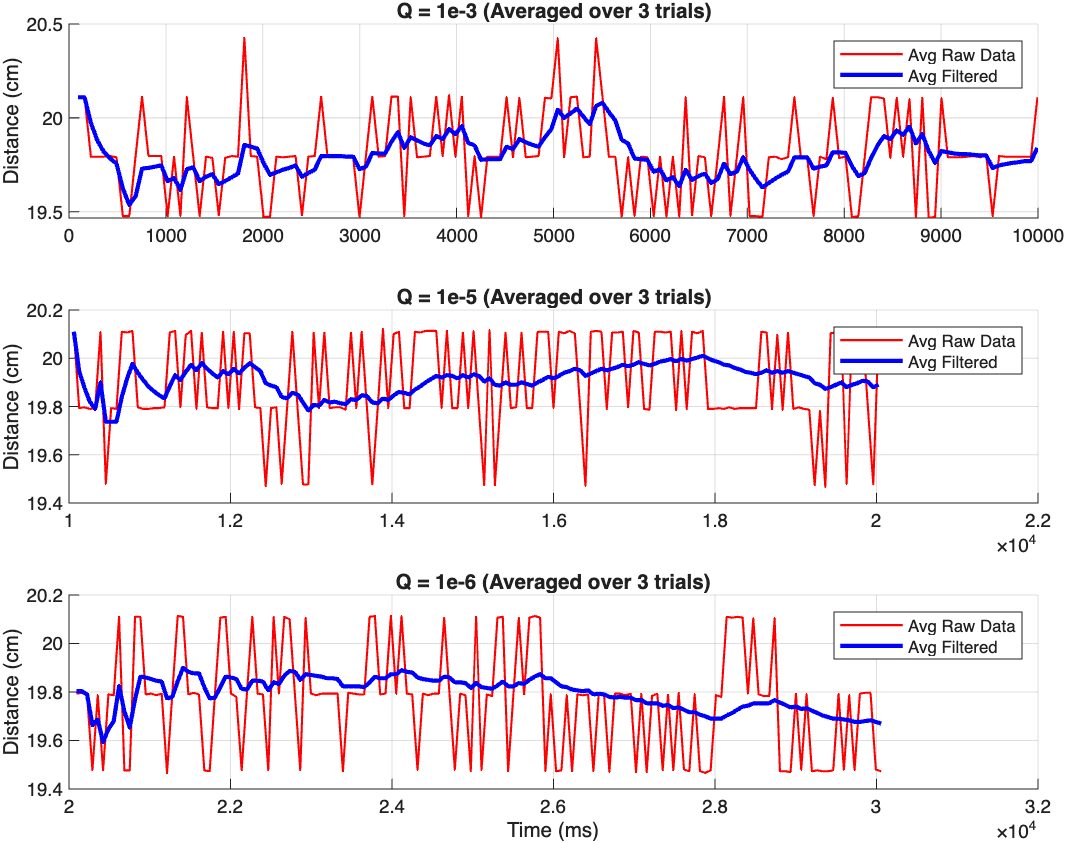
\includegraphics[width=0.85\textwidth]{exp3_scenarioA.png}
    \caption{Time-Domain Plot (Scenario A): Raw Data $z_k$ และ KF Output $\hat{x}_k$
             สำหรับ $Q \in \{1\times10^{-3},\, 1\times10^{-5},\, 1\times10^{-6}\}$
             บนกราฟเดียวกัน ที่ระยะคงที่ 10~cm
             (แกน $x$: เวลา (s), แกน $y$: ระยะทาง (cm))}
    \label{fig:exp3_scenarioA}
\end{figure}

\subsubsection{Scenario B: MSD Free Vibration --- Settling Time และ Variance}

Scenario B ทดสอบพฤติกรรมของ KF ในสภาวะ Dynamic โดยดึงมวลขึ้นจาก
ตำแหน่ง Equilibrium เป็นระยะ $x_0 \approx 7.2$~cm แล้วปล่อย (Free Vibration)
Settling Time นิยามเป็นเวลาที่ KF Output มี Amplitude ของการแกว่ง
ลดลงต่ำกว่า 5\% ของ Initial Amplitude และอยู่ในนั้นตลอดจนสิ้นสุดการบันทึก

\begin{table}[htbp]
    \centering
    \caption{ผลการวัด Settling Time และ Variance Reduction ของ KF
             ในสภาวะ MSD Free Vibration (Scenario B, 3 Trials)}
    \label{tab:exp3_scB_results}
    \begin{tabular}{clcccc}
        \hline
        \textbf{Trial}
            & \textbf{ค่า $Q$}
            & \textbf{Init.\ Amp.\ (cm)}
            & \textbf{Settle (ms)}
            & \textbf{Var KF (cm$^2$)}
            & \textbf{Noise ลดลง (\%)} \\
        \hline
        \multirow{3}{*}{1}
            & $1\times10^{-3}$ & 4.77 & 3232 & 1.2792 & 42.4 \\
            & $1\times10^{-5}$ & 4.59 & 3892 & 0.7948 & 64.2 \\
            & $1\times10^{-6}$ & 4.62 & 3892 & 0.7897 & 64.4 \\
        \hline
        \multirow{3}{*}{2}
            & $1\times10^{-3}$ & 4.95 & 3695 & 1.3223 & 40.3 \\
            & $1\times10^{-5}$ & 4.96 & 4223 & 0.7542 & 65.9 \\
            & $1\times10^{-6}$ & 5.07 & 4685 & 0.7717 & 65.1 \\
        \hline
        \multirow{3}{*}{3}
            & $1\times10^{-3}$ & 4.56 & 3894 & 1.3116 & 42.8 \\
            & $1\times10^{-5}$ & 4.32 & 5214 & 0.7182 & 68.7 \\
            & $1\times10^{-6}$ & 4.36 & 5280 & 0.7114 & 69.0 \\
        \hline
        \multirow{3}{*}{\textbf{Mean}}
            & $1\times10^{-3}$ & 4.76 & \textbf{3607} & 1.3044 & \textbf{41.8} \\
            & $1\times10^{-5}$ & 4.62 & \textbf{4443} & 0.7557 & \textbf{66.3} \\
            & $1\times10^{-6}$ & 4.68 & \textbf{4619} & 0.7576 & \textbf{66.2} \\
        \hline
    \end{tabular}
\end{table}

\begin{figure}[htbp]
    \centering
    % TODO: แทนด้วยกราฟจริงจาก MATLAB (plot ทั้ง 3 Q บนกราฟเดียวกัน)
    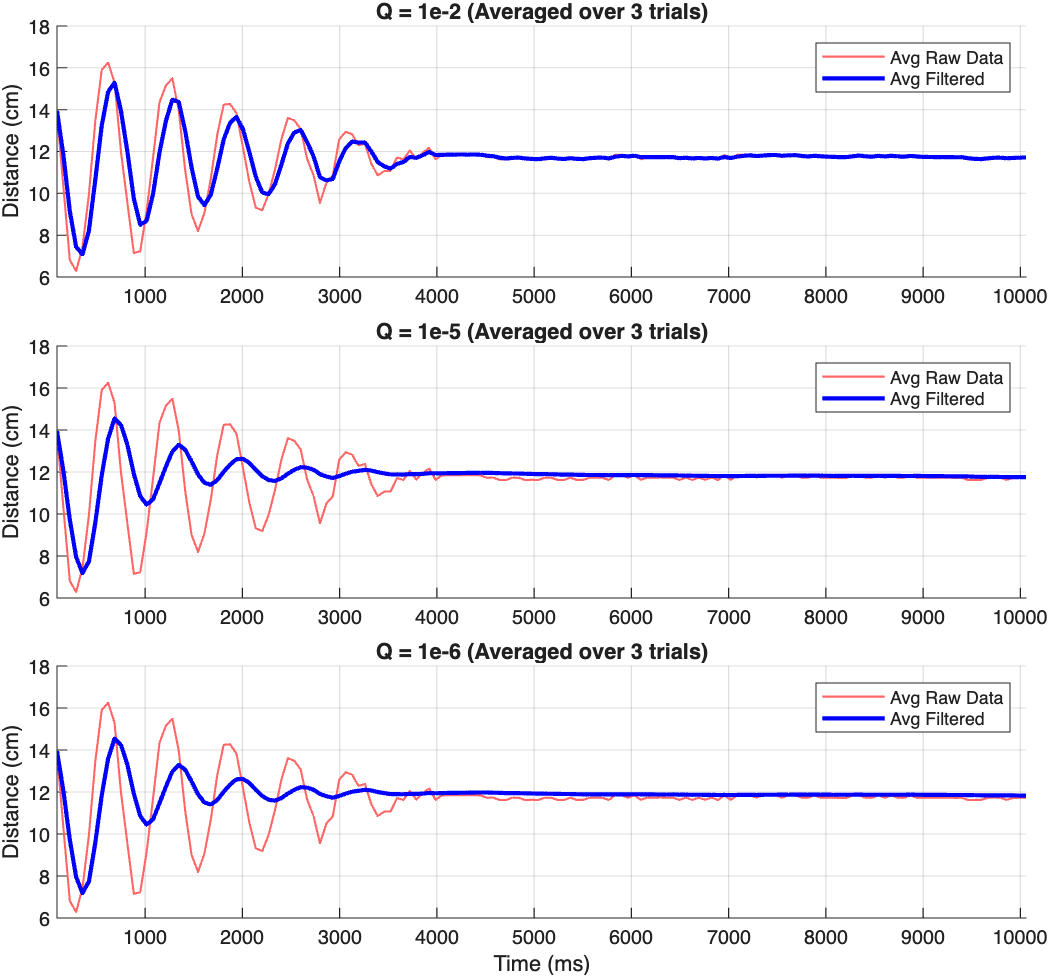
\includegraphics[width=0.85\textwidth]{exp3_scenarioB.png}
    \caption{Time-Domain Plot (Scenario B): Raw Data $z_k$ และ KF Output $\hat{x}_k$
             สำหรับ $Q$ ทั้ง 3 ค่า บนกราฟเดียวกัน
             ระบบ MSD Free Vibration เริ่มต้นที่ $x_0 \approx 7.2$~cm
             จาก Equilibrium
             (แกน $x$: เวลา (s), แกน $y$: ระยะทาง (cm))}
    \label{fig:exp3_scenarioB}
\end{figure}

\subsubsection{สรุปผล Quantitative}

\begin{table}[htbp]
    \centering
    \caption{สรุปค่า Quantitative เปรียบเทียบทั้ง 2 Scenario
             ($R = 0.0337$~cm$^2$, ค่าเฉลี่ยจาก 3 Trials)}
    \label{tab:exp3_summary}
    \begin{tabular}{lcccc}
        \hline
        \textbf{ค่า $Q$}
            & \textbf{$Q/R$}
            & \textbf{$K_{k,\mathrm{ss}}$}
            & \textbf{Settle Time (ms)}
            & \textbf{Var Reduction (\%)} \\
        \hline
        $1\times10^{-3}$ & $2.97\times10^{-2}$ & 0.136 & \textbf{3607} & 41.8 \\
        $1\times10^{-5}$ & $2.97\times10^{-4}$ & 0.017 & 4443          & \textbf{66.3} \\
        $1\times10^{-6}$ & $2.97\times10^{-5}$ & 0.005 & 4619          & 66.2 \\
        \hline
    \end{tabular}
\end{table}

\paragraph{หมายเหตุเกี่ยวกับหน่วย}
กราฟในรูปที่~6 และ~7 แสดงหน่วยแกน $y$ เป็น cm เพื่อความสะดวก
ในการอ่านค่าและเปรียบเทียบ ค่าดังกล่าวสามารถแปลงเป็นหน่วย SI (m)
ได้โดยคูณด้วยตัวประกอบ $1 \times 10^{-2}$
% \begin{figure}[htbp]
%     \centering
%     \includegraphics[width=0.9\textwidth]{figures/Figure_ErrorPlot.pdf}
%     \caption{รูปที่ 8: Error Plot แสดง Residual $e_k = z_k - \hat{x}_k$
%     สำหรับ $Q \in \{1\times10^{-3},\ 1\times10^{-5},\ 1\times10^{-6}\}$
%     ที่ระยะคงที่ 10~cm
%     (แกน $x$: เวลา (s), แกน $y$: Residual ($\times 10^{-2}$~m))}
%     \label{fig:error_plot}
% \end{figure}

%% ─────────────────────────────────────────────────────────────────────────────
\subsection{สรุปผลการทดลอง}

\begin{itemize}
    \item \textbf{Scenario A (Static):} KF ทุกค่า $Q$ สามารถลด Noise ได้อย่าง
          มีนัยสำคัญ (71--99\%) โดย $Q = 1\times10^{-6}$ ให้ Variance Reduction
          สูงที่สุดเฉลี่ย 90.2\% ขณะที่ $Q = 1\times10^{-3}$ ให้ 76.5\%
          สอดคล้องกับทฤษฎีที่ $K_{k,\mathrm{ss}}$ ต่ำกว่าจะกรอง Noise ได้มากกว่า
          แต่แลกกับการตอบสนองที่ช้าลง

    \item \textbf{Scenario B (Dynamic):} $Q = 1\times10^{-3}$ มี Settling Time
          เร็วที่สุดเฉลี่ย 3607~ms เนื่องจาก $K_{k,\mathrm{ss}} = 0.136$
          ทำให้ Filter ติดตาม Measurement ได้ไว แต่ Variance Reduction
          ต่ำที่สุดที่ 41.8\% ขณะที่ $Q = 1\times10^{-5}$ และ $Q = 1\times10^{-6}$
          ให้ Variance Reduction ใกล้เคียงกัน ($\approx 66\%$) แต่ $Q = 1\times10^{-5}$
          settle เร็วกว่า $Q = 1\times10^{-6}$ อย่างชัดเจน (4443 vs.\ 4619~ms)

    \item \textbf{ค่า $Q$ ที่แนะนำ:} $Q = 1\times10^{-5}$ ให้ผลสมดุลดีที่สุด
          ระหว่าง Smoothness (Var Reduction 66.3\%) และ Responsiveness
          (Settle Time 4443~ms) โดยไม่เสียสละ Noise Rejection มากเกินไป
          เหมือน $Q = 1\times10^{-3}$ และตอบสนองได้เร็วกว่า $Q = 1\times10^{-6}$
          อย่างมีนัยสำคัญในสภาวะ Dynamic สอดคล้องกับ Nominal Value
          ที่ Al Tahtawi (2018) เลือกใช้
\end{itemize}

%% ─────────────────────────────────────────────────────────────────────────────
\subsection{อภิปรายผล}

\begin{itemize}
    \item \textbf{กลไกที่ $Q$ ส่งผลต่อ Filter:}
          $Q$ บวกเข้าไปใน $P_k^{(-)}$ ทุกรอบผ่านสมการ~\eqref{eq:cov_predict_exp3}
          ทำให้ Kalman Gain $K_k = P_k^{(-)}/(P_k^{(-)} + R)$ สูงขึ้น
          และ State Update $\hat{x}_k = \hat{x}_k^{(-)} + K_k(z_k - \hat{x}_k^{(-)})$
          ดึง Output เข้าหา Measurement มากขึ้น
          ผลคือ Filter ตอบสนองเร็วขึ้นแต่ยอมรับ Noise จาก Sensor มากขึ้น
          ดังที่เห็นในตารางที่~\ref{tab:exp3_scB_results}
          ว่า $Q = 1\times10^{-3}$ มี Settle Time สั้นที่สุด
          แต่ Variance Reduction ต่ำที่สุด

    \item \textbf{$Q = 1\times10^{-5}$ vs.\ $Q = 1\times10^{-6}$:}
          ผลที่น่าสนใจคือทั้งสองค่านี้ให้ Variance Reduction ใกล้เคียงกันมาก
          ($66.3\%$ vs.\ $66.2\%$) แต่ Settle Time ต่างกัน 176~ms
          เหตุผลคือ $K_{k,\mathrm{ss}}$ ต่างกัน 3.4 เท่า (0.017 vs.\ 0.005)
          ใน Scenario Static ความต่างของ Variance นี้เล็กน้อยเพราะ Signal
          ไม่เปลี่ยนแปลง แต่ใน Dynamic Scenario ความต่างของ Responsiveness
          จะเห็นได้ชัดกว่า

    \item \textbf{$Q/R \ll 1$ ในทุกกรณี:}
          เนื่องจาก $R = 0.0337$~cm$^2$ ใหญ่กว่า $Q$ ทุกค่ามาก
          Filter จึงโน้มเอียงไปทาง ``เชื่อ Model'' เป็นค่า Default อยู่แล้ว
          ซึ่งแตกต่างจาก Al Tahtawi (2018) ที่ใช้ $R = 2.92\times10^{-3}$
          ทำให้ $Q = 1\times10^{-3}$ มี $Q/R > 1$ ในงานวิจัยนั้น
          แต่ \textbf{ทิศทางของ Effect เหมือนกันทุกประการ}
          คือ $Q$ ที่ใหญ่กว่าทำให้ Filter ตอบสนองเร็วกว่าเสมอ

    \item เมื่อเปรียบเทียบกับงานวิจัยของ Al~Tahtawi (2018) ซึ่งใช้
            $R = 2.92\times10^{-3}$~cm$^2$ พบว่าในงานวิจัยนั้น
            $Q = 1\times10^{-3}$ ทำให้ $Q/R > 1$ กล่าวคือ Filter เชื่อ
            Measurement มากกว่า Model ในขณะที่การทดลองนี้ใช้
            $R = 0.0337$~cm$^2$ ซึ่งใหญ่กว่า $Q$ ทุกค่า ทำให้ $Q/R < 1$
            ตลอด Filter จึงโน้มเอียงไปทาง Model มากกว่า อย่างไรก็ตาม
            ทิศทางของ Effect เหมือนกันทุกประการ กล่าวคือ $Q$ ที่ใหญ่กว่า
            ทำให้ Filter ตอบสนองเร็วกว่าเสมอ ไม่ว่า $Q/R$ จะมากกว่าหรือ
            น้อยกว่า 1 ความแตกต่างนี้เกิดจาก Sensor ที่ใช้ในการทดลองนี้
            มี Noise สูงกว่า (Variance ต่างกัน 11 เท่า) ดังนั้นการเปรียบเทียบ
            ค่าสัมบูรณ์ของ $Q$ จึงไม่มีความหมาย แต่ควรเปรียบเทียบจาก
            อัตราส่วน $Q/R$ แทน

    \item \textbf{สภาวะ Overconfident ($Q \to 0$):}
          หาก $Q = 0$ ค่า $P_k$ จะ Converge ลงสู่ศูนย์
          ส่งผลให้ $K_k \rightarrow 0$ ตามสมการ~\eqref{eq:scalar_gain_exp3}
          Filter จะหยุดรับข้อมูลใหม่จาก Sensor โดยสิ้นเชิง
          ซึ่งจะทำให้ KF ไม่สามารถติดตามการแกว่งของ MSD ได้เลย
          แม้แต่ $Q = 1\times10^{-6}$ ที่ใช้ในการทดลองนี้
          ก็ยังแสดงให้เห็นว่า Settle Time ช้ากว่า $Q = 1\times10^{-5}$
          อย่างมีนัยสำคัญในสภาวะ Dynamic

    \item \textbf{ข้อสังเกตเกี่ยวกับ Scenario B:}
          Settling Time ที่วัดได้ในการทดลองนี้สะท้อนทั้งการที่ KF ติดตาม
          Measurement ได้ไวแค่ไหน \textbf{และ} ระยะเวลาที่ระบบ MSD จริง
          Damp Out ทางกายภาพ ดังนั้นความต่างของ Settling Time ระหว่าง
          $Q = 1\times10^{-3}$ (3607~ms) กับ $Q = 1\times10^{-6}$ (4619~ms)
          บางส่วนมาจาก Filter Lag ที่ต่างกัน ไม่ใช่ทั้งหมดจาก Physical Damping
\end{itemize}

\subsection{ข้อเสนอแนะเพื่อการพัฒนา}
 
จากการวิเคราะห์ข้อจำกัดที่พบในการทดลอง มีข้อเสนอแนะเพื่อปรับปรุงและต่อยอดดังนี้
 
\begin{itemize}
    \item \textbf{ขยายช่วงค่า $Q$ ที่ทดสอบ:} การทดลองนี้ทดสอบเพียง 3 ค่าตาม Al Tahtawi (2018) ซึ่งอาจไม่เพียงพอในการหาจุดสมดุลที่เหมาะสมที่สุด ควรทดสอบค่า $Q$ เพิ่มเติมในช่วงระหว่าง $10^{-6}$ ถึง $10^{-3}$ เพื่อให้เห็น Trade-off ระหว่าง Smoothness และ Responsiveness ได้ละเอียดยิ่งขึ้น
    % \item \textbf{วัด Response Time อย่างเป็นระบบ:} การนิยาม Settling Time ผ่าน Envelope Method ในการทดลองนี้มีความซับซ้อน ควรออกแบบ Scenario Step Change ที่ชัดเจนกว่า เช่น เลื่อนวัตถุจาก 10 cm ไปยัง 20 cm อย่างรวดเร็ว เพื่อให้วัด Response Time แบบ 5\% Settling ได้ตรงไปตรงมา
    \item \textbf{พิจารณา Adaptive Process Noise:} ค่า $Q$ คงที่ตลอดเวลาทำให้ Filter ไม่สามารถปรับตัวเมื่อพลศาสตร์ของระบบเปลี่ยน เช่น เมื่อมวลเคลื่อนที่เร็วหรือช้า ในอนาคตอาจพิจารณาใช้ Adaptive Kalman Filter ที่ประมาณค่า $Q$ ใหม่ทุกรอบจาก Innovation Sequence แทน
\end{itemize}
% !TeX root = ../main.tex

\section{การทดลองที่ 4: System Identification ของ Mass-Spring-Damper}
% \textit{ครอบคลุม Criteria: Part 1 System Modeling --- เขียน EOM,
% ออกแบบการทดลองหา $C$, อธิบายหลักการหา $C$, แสดงผล Model Fit (รวม 3 คะแนน)}

%% ─────────────────────────────────────────────────────────────────────────────
%% ─────────────────────────────────────────────────────────────────────────────
\subsection{บทนำ}

ในการสร้างแบบจำลองทางคณิตศาสตร์ (State-Space Model) ของระบบ Mass-Spring-Damper (MSD) เพื่อนำไปใช้ออกแบบตัวประมาณค่าสถานะ (State Estimator) นั้น ความแม่นยำของพารามิเตอร์ทางกายภาพคือหัวใจสำคัญ จากการทดลองที่ 1 ได้ประเมินค่า Spring Constant เบื้องต้นไว้ที่ $K = 29.11$~N/m อย่างไรก็ตาม แบบจำลองจะสมบูรณ์ได้จำเป็นต้องทราบพารามิเตอร์ที่ควบคุมอัตราการสูญเสียพลังงานของระบบด้วย นั่นคือ Damping Coefficient ($C$) 

การหาค่า $C$ มีความซับซ้อนกว่าการหาค่า $K$ ด้วยเหตุผลทางพลศาสตร์ดังต่อไปนี้:
\begin{itemize}
    \item \textbf{ข้อจำกัดในการวัดโดยตรง:} แตกต่างจากแรงสปริงที่ขึ้นอยู่กับระยะตำแหน่ง (Position) แรงหน่วงในระบบเป็นสัดส่วนโดยตรงกับความเร็ว (Velocity) ซึ่งวัดค่าแบบสถิต (Static) ไม่ได้
    \item \textbf{ความซับซ้อนของแรงเสียดทาน:} ในระบบกลไกจริง พารามิเตอร์ $C$ ไม่ได้เกิดจากตัวหน่วงอากาศเพียงอย่างเดียว แต่ยังรวมผลกระทบจากแรงเสียดทาน (Coulomb และ Viscous Friction) ที่แฝงอยู่ในระบบด้วย
\end{itemize}



ดังนั้น วิธีที่เหมาะสมที่สุดคือการทำ \textbf{System Identification} โดยการออกแบบการทดลองสภาวะการสั่นอย่างอิสระ (Free Vibration) คือการดึงมวลออกจากจุดสมดุล (Equilibrium) แล้วปล่อยโดยไม่มีแรงภายนอกมากระทำ ทำให้ $F(t) = 0$ สมการการเคลื่อนที่ (EOM) จึงลดรูปเหลือความสัมพันธ์ระหว่าง $m$, $K$, และ $C$ จากนั้นบันทึกการตอบสนองของระบบจริง (Measured Data) เพื่อนำไปวิเคราะห์ย้อนกลับ

\textbf{การปรับปรุงแนวทางการประเมินพารามิเตอร์ (Parameter Estimation Strategy):}
\begin{itemize}
    \item ในเบื้องต้น ทฤษฎีกำหนดให้ยึดค่า $m$ และ $K$ คงที่ เพื่อค้นหาค่า $C$ เพียงตัวเดียว
    \item อย่างไรก็ตาม ในการทดลองที่ 4 และ 5 ได้มีการปรับเปลี่ยนชุดทดลองโดยเพิ่ม \textbf{เสาไกด์ (Guide Rail)} แนบชิดกับฐานมวลเพื่อให้เซนเซอร์อ่านค่าได้เสถียรขึ้น การสัมผัสนี้ทำให้เกิดแรงต้านทานเพิ่มเติมและส่งผลให้แนวการรับแรงดิ่งของสปริงเปลี่ยนแปลงไปจากสภาวะอิสระของการทดลองที่ 1
    \item เพื่อป้องกันความคลาดเคลื่อนของแบบจำลอง (Model Mismatch) การทดลองนี้จึงใช้ MATLAB Parameter Estimator ในการ\textbf{ค้นหาค่า $C$ และปรับแก้ค่า $K$ ไปพร้อมกัน} โดยให้ Algorithm ทำการ Optimization จนกว่าผลการจำลอง (Simulation) จะสอดคล้องกับข้อมูลที่วัดได้จริงมากที่สุด (Best Fit)
\end{itemize}

พารามิเตอร์ $K$ ที่อัปเดตใหม่ และค่า $C$ (Effective Damping) ที่ครอบคลุมแรงต้านทานทั้งหมดในระบบ จะถูกนำไปใช้สร้างเมทริกซ์พลวัต (Discrete State Matrix, $A_d$) สำหรับ 2-State Kalman Filter ในการทดลองที่ 5 ต่อไป
%% ─────────────────────────────────────────────────────────────────────────────
\subsection{วัตถุประสงค์}

\begin{itemize}
    \item เพื่อ Derive และเขียน Equation of Motion (EOM) ของระบบ
          Mass-Spring-Damper จาก Newton's Second Law อย่างสมบูรณ์
    \item เพื่อออกแบบการทดลอง Free Vibration ที่เหมาะสม
          สำหรับการเก็บข้อมูล Displacement เพื่อนำไป Identify พารามิเตอร์
    \item เพื่อประมาณค่า Damping Coefficient $C$ โดยใช้
          MATLAB Parameter Estimator (Simulink Design Optimization)
    \item เพื่อตรวจสอบความถูกต้องของ Model โดยเปรียบเทียบผลการ Simulate
          กับข้อมูลจริงผ่าน Fit Metrics
\end{itemize}

%% ─────────────────────────────────────────────────────────────────────────────
\subsection{สมมติฐาน}

\begin{itemize}
    \item การตอบสนองของระบบภายใต้ Free Vibration จะมีลักษณะ Under-Damped Second-Order Response ($\zeta < 1$) เนื่องจากระบบ MSD ในชุดทดลองนี้มีการแกว่งที่สังเกตได้ชัดเจน
    \item Parameter Estimator จะค้นพบค่า $K$ ที่เปลี่ยนไปจากเดิมเล็กน้อย และค่า $C$ ที่ครอบคลุมทั้งแรงต้านอากาศและแรงเสียดทาน (Friction) จากเสาไกด์
    \item ค่าพารามิเตอร์ทั้งสองที่ประเมินได้ เมื่อประกอบกับมวล $m$ จะสามารถสร้างแบบจำลองที่จำลองพฤติกรรมของระบบจริงได้อย่างแม่นยำ
\end{itemize}

%% ─────────────────────────────────────────────────────────────────────────────
\subsection{ตัวแปร}

\begin{itemize}
    \item \textbf{ตัวแปรอิสระ:} Initial Displacement $x_0$ (m) คือจุดที่สปริงหดจากจุด Equilibrium (ประมาณ 7.2 cm)
    \item \textbf{ตัวแปรตาม:} Displacement ตามเวลา $x(t)$ วัดด้วย HC-SR04, \textbf{ค่า Spring Constant $K$ (N/m) และ Damping Coefficient $C$ (N$\cdot$s/m) ที่ประเมินได้}, Damping Ratio $\zeta$
    \item \textbf{ตัวแปรควบคุม:} มวล $m$ (kg) คงที่ตลอดการทดลอง, Sampling Time 10~ms, ความเร็วเริ่มต้น $\dot{x}(0) = 0$
\end{itemize}

%% ─────────────────────────────────────────────────────────────────────────────
\subsection{เอกสารและงานวิจัยที่เกี่ยวข้อง}

\subsubsection{Equation of Motion ของ Mass-Spring-Damper}

เมื่อพิจารณามวล $m$ ในระบบ Mass-Spring-Damper แบบแนวดิ่ง
\begin{figure}[htbp]
    \centering
    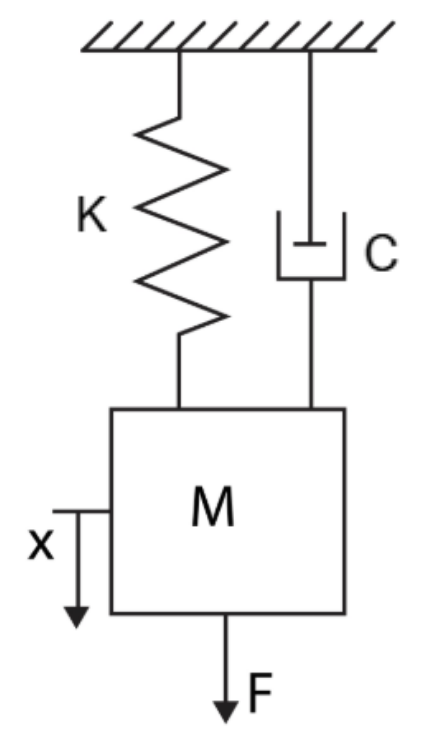
\includegraphics[width=0.3\textwidth]{exp4_fbd_msd.png}
    \caption{Free Body Diagram ของมวลในระบบ Mass-Spring-Damper
             แสดงแรงที่กระทำต่อมวลในทิศทาง $x$ (แนวดิ่ง)}
    \label{fig:fbd_msd}
\end{figure}    
มีแรงกระทำต่อมวล 3 แรงหลัก ได้แก่ แรงจากสปริง $-Kx$,
แรงหน่วง $-C\dot{x}$, และแรงภายนอก $F(t)$
เมื่อนำ Newton's Second Law ($\Sigma F = ma$) มาใช้จะได้:

\begin{equation}
    m\ddot{x} = -Kx - C\dot{x} + F(t)
    \label{eq:newton_msd}
\end{equation}

จัดรูปใหม่ได้ EOM มาตรฐานของระบบ Second-Order:

\begin{equation}
    m\ddot{x} + C\dot{x} + Kx = F(t)
    \label{eq:eom_msd}
\end{equation}

โดยที่ $m$ คือมวล (kg), $C$ คือ Damping Coefficient (N$\cdot$s/m),
$K$ คือ Spring Constant (N/m), $x$ คือการกระจัดจาก Equilibrium (m),
และ $F(t)$ คือแรงภายนอก (N) ซึ่งในกรณี Free Vibration มีค่า $F(t) = 0$

\subsubsection{เหตุผลที่ใช้ Displacement จาก Equilibrium เป็น State}

ในการสร้างแบบจำลองทางคณิตศาสตร์ การเลือกจุดอ้างอิง (Reference Point) มีผลอย่างมากต่อความซับซ้อนของสมการ State-Space เพื่อให้เข้าใจถึงประโยชน์ของการใช้ "การกระจัดจากจุดสมดุล" ($x$) แทน "ตำแหน่งสัมบูรณ์" ($x_\text{abs}$) สามารถพิจารณาได้จากลำดับดังต่อไปนี้



\textbf{1. นิยามของจุดอ้างอิงทางกายภาพ}
\begin{itemize}
    \item \textbf{$x_\text{abs}$ (Absolute Position):} ตำแหน่งที่วัดจากจุดที่สปริงยังไม่ยืดตัว (Unstretched Position)
    \item \textbf{$x_\text{eq}$ (Static Deflection):} ระยะยืดสถิต ซึ่งเป็นจุดที่มวลแขวนอยู่นิ่งๆ โดยที่แรงสปริงดึงกลับมีค่าเท่ากับน้ำหนักของมวลพอดี ($K x_\text{eq} = mg$)
    \item \textbf{$x$ (Displacement):} การกระจัดที่วัดจากจุดสมดุลใหม่ ซึ่งมีความสัมพันธ์คือ $x = x_\text{abs} - x_\text{eq}$
\end{itemize}

\textbf{2. การลดรูปสมการคณิตศาสตร์}

หากพิจารณา EOM โดยใช้ตำแหน่งสัมบูรณ์ $x_\text{abs}$ จะมีแรงโน้มถ่วง $mg$ ปรากฏเป็นค่าคงที่ในสมการ:
\begin{equation}
    m\ddot{x}_\text{abs} + C\dot{x}_\text{abs} + K x_\text{abs} = mg
    \label{eq:eom_absolute}
\end{equation}

เนื่องจากระยะ $x_\text{eq}$ เป็นค่าคงที่ การหาอนุพันธ์เทียบกับเวลาจึงมีค่าเท่ากับศูนย์ ส่งผลให้ความเร็วและความเร่งในทั้งสองระบบพิกัดมีค่าเท่ากัน ($\dot{x} = \dot{x}_\text{abs}$ และ $\ddot{x} = \ddot{x}_\text{abs}$) เมื่อแทนค่า $x_\text{abs} = x + x_\text{eq}$ ลงในสมการ~\eqref{eq:eom_absolute} จะได้:
\begin{equation}
    m\ddot{x} + C\dot{x} + K(x + x_\text{eq}) = mg
\end{equation}

กระจายเทอม $K$ และแทนค่าความสัมพันธ์สถิตยศาสตร์ $K x_\text{eq} = mg$:
\begin{equation}
    m\ddot{x} + C\dot{x} + Kx + mg = mg \quad \Rightarrow \quad m\ddot{x} + C\dot{x} + Kx = 0
    \label{eq:equilibrium_cancel}
\end{equation}

\textbf{3. ประโยชน์ในเชิงวิศวกรรมควบคุม (Control Theory)}

การที่เทอม $mg$ หายไปจากสมการ~\eqref{eq:equilibrium_cancel} มีนัยสำคัญอย่างมากต่อการออกแบบตัวควบคุมและตัวประมาณค่า:
\begin{itemize}
    \item \textbf{หลีกเลี่ยง Constant Disturbance:} หากใช้ $x_\text{abs}$ สมการ State-Space จะอยู่ในรูป $\dot{X} = AX + Bu + D$ (โดย $D$ คือเวกเตอร์ของแรงโน้มถ่วง) ซึ่งทำให้ระบบสูญเสียความเป็น Linear Homogeneous การแก้ปัญหานี้บังคับให้เราต้องถือว่าแรงโน้มถ่วงเป็น Input ($u$) ค่าคงที่ตลอดเวลา ซึ่งสร้างความซับซ้อนให้กับระบบเมทริกซ์โดยไม่จำเป็น
    \item \textbf{ลดความซับซ้อนของ Kalman Filter:} เมื่อย้ายจุดกำเนิดมาที่จุดสมดุล แรงโน้มถ่วงจะถูก "หักล้าง" ด้วยแรงตึงสปริงเริ่มต้น (Pre-load) ไปแล้ว ระบบจะเหลือเพียงพฤติกรรมทางพลศาสตร์ (Dynamic Behavior) ล้วนๆ ทำให้ State-Space Model อยู่ในรูปแบบ $\dot{X} = AX$ มาตรฐาน ส่งผลให้การเขียนโค้ดสำหรับ Prediction Step ใน Kalman Filter ตรงไปตรงมา และไม่ต้องเขียนอัลกอริทึมจัดการ Input Offset ชดเชยแรงโน้มถ่วงเพิ่มเติม
\end{itemize}
\subsubsection{Damping Ratio และประเภทของ Response}

Damping Ratio $\zeta$ เป็นพารามิเตอร์ไร้มิติที่บอกว่าระบบสูญเสียพลังงาน
และหยุดการแกว่งได้เร็วแค่ไหน นิยามโดยเปรียบเทียบ $C$ จริงกับ
Critical Damping Coefficient $C_c = 2\sqrt{Km}$:

\begin{equation}
    \zeta = \frac{C}{C_c} = \frac{C}{2\sqrt{Km}}
    \label{eq:damping_ratio}
\end{equation}

และ Natural Frequency $\omega_n$ นิยามเป็น:

\begin{equation}
    \omega_n = \sqrt{\frac{K}{m}}
    \label{eq:natural_freq}
\end{equation}

ค่า $\zeta$ กำหนดลักษณะของ Response โดยตรง:

\begin{figure}[htbp]
    \centering
    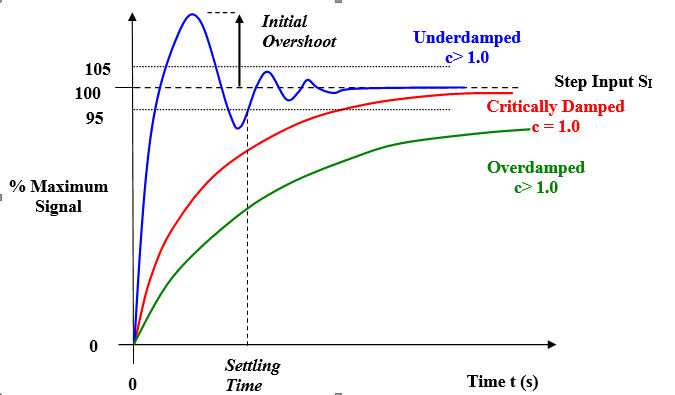
\includegraphics[width=0.7\textwidth]{exp4_damp_ratio.png}
    \caption{ลักษณะของการตอบสนองของระบบแบบ Step Input
             ตามค่า Damping Ratio $\zeta$}
    \label{fig:damp_ratio}
\end{figure}    

\begin{itemize}
    \item \textbf{Under-Damped ($\zeta < 1$):} ระบบแกว่งข้าม Equilibrium
          ไปมา โดยแอมพลิจูดลดลงแบบ Exponential จนหยุดนิ่ง
          รากของสมการลักษณะเฉพาะเป็นจำนวนเชิงซ้อน Conjugate
    \item \textbf{Critically-Damped ($\zeta = 1$):} ระบบกลับสู่ Equilibrium
          เร็วที่สุดโดยไม่มีการแกว่ง รากซ้ำกัน (Real and Repeated Roots)
    \item \textbf{Over-Damped ($\zeta > 1$):} ระบบไม่แกว่ง แต่กลับสู่
          Equilibrium ช้ากว่า Critically-Damped
          รากต่างกัน (Real and Distinct Roots)
\end{itemize}

\subsubsection{MATLAB Parameter Estimator (Simulink Design Optimization)}

MATLAB Parameter Estimator ทำงานโดยใช้ Algorithm ทางคณิตศาสตร์
(เช่น Nonlinear Least Squares) เพื่อค้นหาค่าพารามิเตอร์ที่ทำให้
ผลต่างระหว่าง Simulation กับข้อมูลจริงมีค่าน้อยที่สุด
โดยใช้ Objective Function:

\begin{equation}
    J(K,\,C) = \sum_{k=1}^{N}
               \left[ x_\text{measured}(t_k)
                    - x_\text{simulated}(t_k;\,K,\,C) \right]^2
    \label{eq:param_est_cost}
\end{equation}

แม้ว่าการทดลองที่ 1 จะได้ค่า $K = 29.11$ N/m มาแล้ว
แต่เนื่องจากการทดลองที่ 4 ใช้ Setup ที่ต่างออกไปโดยมีการเพิ่ม
Guide Rail เพื่อบังคับให้มวลเคลื่อนที่ในแนวดิ่งอย่างเคร่งครัด
การเปลี่ยนแปลงนี้ทำให้แนวการรับแรงของสปริงเปลี่ยนไป
ส่งผลให้ค่า $K$ ที่มีผลต่อพลศาสตร์ในแนวดิ่งเปลี่ยนแปลงตามด้วย
ดังนั้นจึงตัดสินใจปล่อยให้ Estimator ค้นหาค่า $K$ และ $C$ พร้อมกัน
เพื่อให้ได้พารามิเตอร์ที่สอดคล้องกับ Setup จริงของการทดลองนี้
มากที่สุด แทนที่จะ Fix $K$ ไว้ที่ค่าเดิมซึ่งวัดจาก Setup ที่ต่างกัน

Algorithm จะค้นหาคู่ $(K,\,C)$ ที่ทำให้ $J(K,C)$ มีค่าต่ำที่สุด
สำหรับการสร้าง Simulink Model ต้องจัดรูป EOM
ให้อยู่ในรูปที่แก้หาความเร่งได้:

\begin{equation}
    \ddot{x} = \frac{1}{m}\!\left(-C\dot{x} - Kx\right)
    \quad \text{(กรณี Free Vibration: }F(t) = 0\text{)}
    \label{eq:simulink_accel}
\end{equation}

จากนั้น Define State $v = \dot{x}$ เพื่อแปลงเป็น First-Order
State Equations สำหรับ Simulink:

\begin{equation}
    \dot{x} = v, \qquad
    \dot{v} = \frac{-Cv - Kx}{m}
    \label{eq:simulink_state}
\end{equation}

\subsection{การปรับปรุง Setup การทดลอง}
 
ในการทดลองที่ 1 สปริงถูกติดตั้งอย่างอิสระ ทำให้มวล (ฐานหนัก $m = 0.290$~kg)
มีโอกาสแกว่งออกนอกแนวดิ่งเล็กน้อย ส่งผลให้ HC-SR04
อ่านค่าระยะทางได้คลาดเคลื่อน เนื่องจากลำคลื่นอัลตราโซนิคต้องการพื้นผิวสะท้อน
ที่ตั้งฉากกับทิศทางการส่งคลื่น
 
การทดลองที่ 4 จึงปรับ Setup ใหม่โดยขยับเสาไกด์ (Guide Rail) เข้ามาชิดกับ
ฐานมวล ทำให้ฐานขนานกับพื้นและเคลื่อนที่ในแนวดิ่งได้ตรงยิ่งขึ้น
ส่งผลให้ Sensor อ่านค่าได้เสถียร อย่างไรก็ตาม การที่ฐานสัมผัสกับเสาไกด์
ทำให้เกิดแรงเสียดทาน (Friction) ในแนวดิ่งเพิ่มเติม ซึ่งส่งผลสองประการดังนี้
 
\begin{itemize}
    \item \textbf{ค่า $C$ ที่ Estimate ได้สูงกว่าความเป็นจริงของ Damper อย่างเดียว:}
          $C_\text{eff}$ ที่ได้จาก Parameter Estimator สะท้อนผลรวมของ
          Damping จริงของ Damper และ Friction ของ Guide Rail
          จึงถือเป็น Effective Damping Coefficient
          ที่ตรงกับระบบที่ใช้ในการทดลองที่ 5 มากที่สุด
 
    \item \textbf{ค่า $K$ ที่ Estimate ได้เปลี่ยนจาก Exp 1:}
          การปรับ Setup ทำให้ระยะ Pre-load ของสปริงและแนวการรับแรงเปลี่ยนไปบางส่วน
          ดังนั้น Parameter Estimator จึง Estimate ทั้ง $K$ และ $C$
          พร้อมกันจากข้อมูล Free Vibration จริงของ Setup นี้
          แทนที่จะ Fix $K = 29.11$~N/m จากการทดลองที่ 1
\end{itemize}
 
Simulink Model ที่สร้างขึ้นสอดคล้องกับ Setup นี้ โดย Output ของ Model
คือ Absolute Distance จาก Sensor (cm) ไม่ใช่ Displacement จาก Equilibrium
จึงต้องบวก Offset $x_\text{eq} = 11.3$~cm เข้าไปใน Model
ตามระยะที่ Sensor อ่านได้ที่ตำแหน่ง Equilibrium จริง

\subsubsection{การวิเคราะห์และคัดกรองข้อมูลผิดปกติ (Outlier Analysis)}

ในการทดลองทางวิศวกรรมและการระบุพารามิเตอร์ของระบบ (System Identification) ข้อมูลที่ได้จากการทดลองซ้ำ (Multiple Trials) มักมีการกระจายตัวอยู่ในช่วงระดับหนึ่งเนื่องจากสัญญาณรบกวน (Noise) และความไม่แน่นอนของระบบ อย่างไรก็ตาม ในบางกรณีอาจเกิด "ข้อมูลผิดปกติ" (Outlier) ซึ่งเป็นจุดข้อมูลที่มีค่าเบี่ยงเบนออกไปจากกลุ่มข้อมูลส่วนใหญ่อย่างสุดโต่ง สาเหตุอาจเกิดจากความผิดพลาดชั่วขณะของเซนเซอร์ การรบกวนจากสภาพแวดล้อม หรือพฤติกรรมทางกายภาพที่ผิดปกติ (เช่น การที่ฐานมวลเสียดสีกับเสาไกด์อย่างรุนแรงในบางรอบการทดลอง) 

หากนำข้อมูลที่เป็น Outlier มาร่วมคำนวณหาค่าเฉลี่ย (Mean) หรือความแปรปรวน (Variance) จะทำให้ค่าสถิติเหล่านั้นบิดเบือนไปจากความเป็นจริง (Skewed) ส่งผลให้แบบจำลองทางคณิตศาสตร์มีความคลาดเคลื่อน ดังนั้นจึงต้องมีกระบวนการทางสถิติที่น่าเชื่อถือในการตรวจจับและคัดกรองข้อมูลเหล่านี้ออกก่อนนำไปใช้งาน

\begin{figure}[htbp]
    \centering
    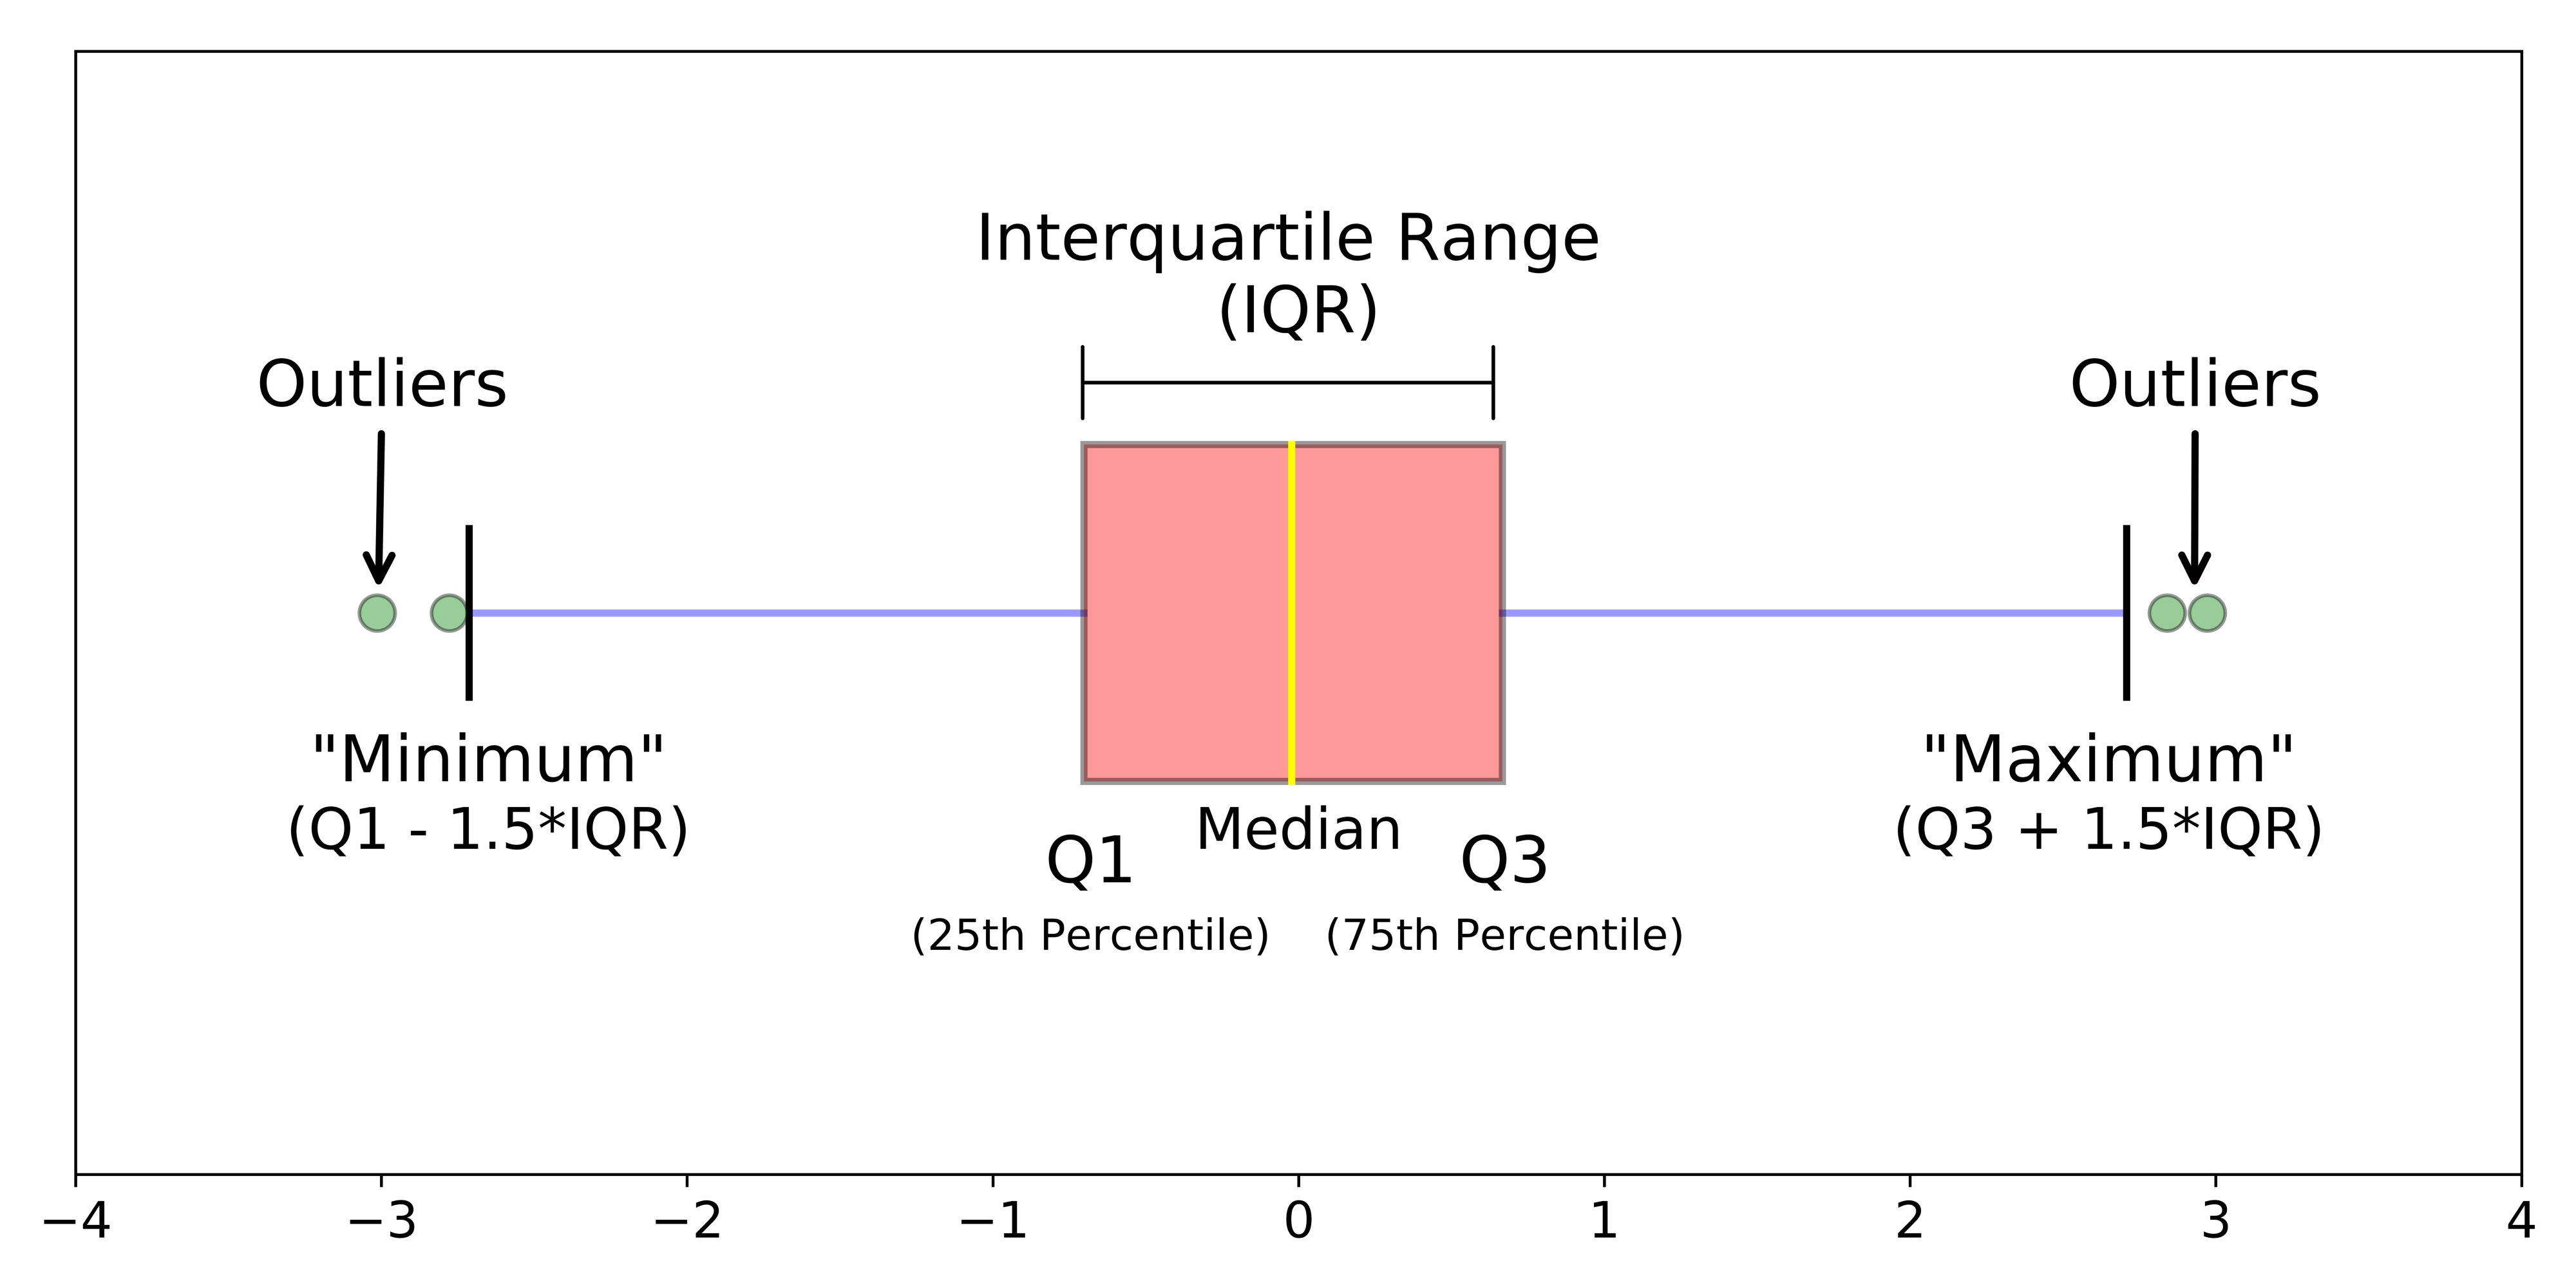
\includegraphics[width=0.7\textwidth]{bloxplot.png} 
    \caption{การวิเคราะห์ข้อมูลผิดปกติ (Outlier Analysis) ของค่า Damping Coefficient $C$ ด้วยวิธี Interquartile Range (IQR)}
    \label{fig:outlier_boxplot}
\end{figure}

\textbf{วิธีการพิสัยระหว่างควอร์ไทล์ (Interquartile Range: IQR)}
วิธี IQR เป็นเครื่องมือทางสถิติที่ได้รับความนิยมอย่างแพร่หลายในการระบุตำแหน่งของ Outlier เนื่องจากเป็นวิธีที่ทนทาน (Robust) ต่อข้อมูลที่มีความเบ้ (Skewness) และไม่จำเป็นต้องตั้งสมมติฐานว่าข้อมูลมีการแจกแจงแบบปกติ (Normal Distribution) โดยมีหลักการและขั้นตอนทางคณิตศาสตร์ดังนี้:

\begin{itemize}
    \item \textbf{การหาตำแหน่งควอร์ไทล์ (Quartiles):} นำชุดข้อมูลมาเรียงลำดับจากน้อยไปมาก จากนั้นแบ่งข้อมูลออกเป็น 4 ส่วนเท่าๆ กัน ค่าที่แบ่งส่วนที่ 1 และ 2 คือ ควอร์ไทล์ที่ 1 ($Q_1$ หรือ 25th Percentile) และค่าที่แบ่งส่วนที่ 3 และ 4 คือ ควอร์ไทล์ที่ 3 ($Q_3$ หรือ 75th Percentile)
    \item \textbf{การคำนวณระยะ IQR:} พิสัยระหว่างควอร์ไทล์คือระยะห่างระหว่าง $Q_3$ และ $Q_1$ ซึ่งครอบคลุมช่วงข้อมูลกึ่งกลาง 50\% ของข้อมูลทั้งหมด
    \begin{equation}
        \text{IQR} = Q_3 - Q_1
        \label{eq:iqr_calc}
    \end{equation}
    \item \textbf{การสร้างขอบเขต (Fences):} ใช้ระยะ IQR ในการกำหนดขอบเขตบนและล่างสำหรับคัดกรองข้อมูล โดยทั่วไปนิยมใช้ตัวคูณ 1.5 สำหรับข้อมูลผิดปกติระดับมาตรฐาน (Mild Outliers) 
    \begin{align}
        \text{Lower Fence} &= Q_1 - 1.5 \times \text{IQR} \label{eq:lower_fence} \\
        \text{Upper Fence} &= Q_3 + 1.5 \times \text{IQR} \label{eq:upper_fence}
    \end{align}
    \item \textbf{เกณฑ์การตัดสิน:} ข้อมูลใดๆ ที่มีค่าน้อยกว่า Lower Fence หรือมีค่ามากกว่า Upper Fence จะถูกพิจารณาว่าเป็น Outlier ทางสถิติ และมีความชอบธรรมทางวิชาการที่จะถูกแยกออกจากการคำนวณพารามิเตอร์ของระบบ
\end{itemize}

%% ─────────────────────────────────────────────────────────────────────────────
\subsection{ขั้นตอนการทดลอง}

\textbf{ส่วนที่~1: เตรียมชุดทดลองและเก็บข้อมูล Free Vibration}

\begin{enumerate}
    \item ประกอบชุด Mass-Spring-Damper \textbf{โดยปรับเสาไกด์ให้แนบกับฐานมวลพอดี} วาง HC-SR04 ด้านล่างชี้ขึ้นเพื่อวัด Displacement ในแนวดิ่ง
    \item ชั่งมวล $m$ ด้วยเครื่องชั่ง บันทึกค่าเป็น kg
    \item ตั้งระบบให้มวลอยู่ที่ Equilibrium Position ยืนยันว่า HC-SR04 อ่านค่า Baseline คงที่ กำหนดตำแหน่งนี้เป็น $x = 0$
    \item ดึงมวลขึ้นจาก Equilibrium เป็นระยะประมาณ 7.2 cm จนสปริงหดแล้วปล่อยโดยไม่ออกแรง ($\dot{x}(0) = 0$) บันทึก Oscillation จนกว่าจะ Damp Out ส่งข้อมูลผ่าน Serial 115200 baud
    \item ทำซ้ำการ Release 5 ครั้งเพื่อตรวจสอบ Repeatability บันทึกทุก Dataset แยกไฟล์
\end{enumerate}

\textbf{ส่วนที่~2: System Identification ด้วย MATLAB Parameter Estimator}

\begin{enumerate}
    \item Import ข้อมูล Displacement จาก Serial ลงใน MATLAB แปลงหน่วยเป็นเมตร
    \item สร้าง Simulink Model ของ MSD โดยใช้ State Equations: Input $u = 0$, Initial Condition $x(0) = x_0$, $v(0) = 0$
    \item เปิด Simulink Design Optimization \textbf{กำหนดให้ $K$ และ $C$ เป็น Parameter ที่ต้องการ Estimate พร้อมกัน} โดยตั้งค่าเริ่มต้น (Initial Guess) ของ $K = 29.11$~N/m (จาก Exp 1) และ Fix ค่า $m$ ไว้
    \item รัน Estimator จนกว่าจะ Converge บันทึกค่า $K$ และ $C$ ที่ได้
    \item คำนวณ $\zeta$ จากสมการ $\zeta = C / (2\sqrt{Km})$ และจัดประเภท Damping
    \item Overlay กราฟ Model Simulation กับ Measured Data บันทึกค่า RMSE และทำ Outlier Analysis
\end{enumerate}

\subsection{ผลการทดลอง}
 
\subsubsection{Equation of Motion}
 
จาก Newton's Second Law สำหรับระบบ Mass-Spring-Damper
ที่ใช้ Displacement จาก Equilibrium เป็น State:
 
\begin{equation}
    m\ddot{x} + C\dot{x} + Kx = 0
    \quad \text{(Free Vibration)}
    \label{eq:eom_free_vib}
\end{equation}
 
% โดยพารามิเตอร์ที่ทราบจากการทดลองที่ 1: $K_\text{Exp1} = 29.11$~N/m
% และมวล $m = 0.290$~kg
\subsubsection{Outlier Analysis ของผล Parameter Estimation}
 
จากการทำซ้ำ 5 Trials พบว่าค่า $C$ ของ Trial 8 มีค่าสูงผิดปกติ
จึงทำการตรวจสอบด้วยวิธี IQR (Interquartile Range)
 
\begin{table}[htbp]
    \centering
    \caption{ผลการ Estimate พารามิเตอร์ $K$ และ $C$ จาก 5 Trials
             (MATLAB Parameter Estimator, Simulink Design Optimization)}
    \label{tab:param_est_raw}
    \begin{tabular}{cccc}
        \hline
        \textbf{Trial} & \textbf{$K$ (N/m)} & \textbf{$C$ (N$\cdot$s/m)} & \textbf{หมายเหตุ} \\
        \hline
        1 & 33.5482 & 0.3961 & --- \\
        4 & 31.4963 & 0.3760 & --- \\
        5 & 33.2512 & 0.4184 & --- \\
        7 & 29.8704 & 0.3623 & --- \\
        8 & 30.9629 & 0.9792 & Outlier (IQR) \\
        \hline
    \end{tabular}
\end{table}
 
การตรวจสอบ Outlier ด้วยวิธี IQR สำหรับค่า $C$
มีขั้นตอนดังนี้
 
\begin{enumerate}
    \item เรียงค่า $C$ จากน้อยไปมาก:
          $\{0.3623,\; 0.3760,\; 0.3961,\; 0.4184,\; 0.9792\}$
    \item คำนวณ Quartile:
          $Q_1 = 0.3760$, $Q_3 = 0.4184$,
          $\text{IQR} = Q_3 - Q_1 = 0.0424$
    \item กำหนด Fence:
          \begin{align}
              \text{Lower fence} &= Q_1 - 1.5 \times \text{IQR}
                                  = 0.3760 - 0.0635 = 0.3125 \notag \\
              \text{Upper fence} &= Q_3 + 1.5 \times \text{IQR}
                                  = 0.4184 + 0.0635 = 0.4819 \notag
          \end{align}
    \item Trial 8 มีค่า $C = 0.9792 > 0.4819$ จึงถือเป็น Outlier
          และตัดออกจากการคำนวณค่าเฉลี่ย
\end{enumerate}
 
\subsubsection{สถิติของพารามิเตอร์ที่ได้}
 
\begin{table}[htbp]
    \centering
    \caption{สถิติของ $K$ และ $C$ ก่อนและหลังตัด Outlier}
    \label{tab:param_stats}
    \begin{tabular}{lccccc}
        \hline
        \textbf{กลุ่ม} & \textbf{$n$}
            & \textbf{$\bar{K}$ (N/m)} & \textbf{S.D.($K$)}
            & \textbf{$\bar{C}$ (N$\cdot$s/m)} & \textbf{S.D.($C$)} \\
        \hline
        ทั้งหมด (5 Trials) & 5 & 31.83 & 1.56 & 0.5064 & 0.2652 \\
        ไม่รวม Trial 8     & 4 & 32.04 & 1.71 & 0.3882 & 0.0245 \\
        \hline
    \end{tabular}
\end{table}
 
การตัด Outlier ทำให้ S.D. ของ $C$ ลดลงจาก 0.2652 เป็น 0.0245~N$\cdot$s/m
(ลดลง 90.8\%) ขณะที่ S.D. ของ $K$ ไม่เปลี่ยนแปลงมากนัก
ยืนยันว่า Trial 8 มีผลกระทบต่อ $C$ อย่างมีนัยสำคัญ
 
\subsubsection{Simulink Model และ Parameter Estimator}
 
\begin{figure}[htbp]
    \centering
    % TODO: แทนด้วยรูป Simulink Model จริง
    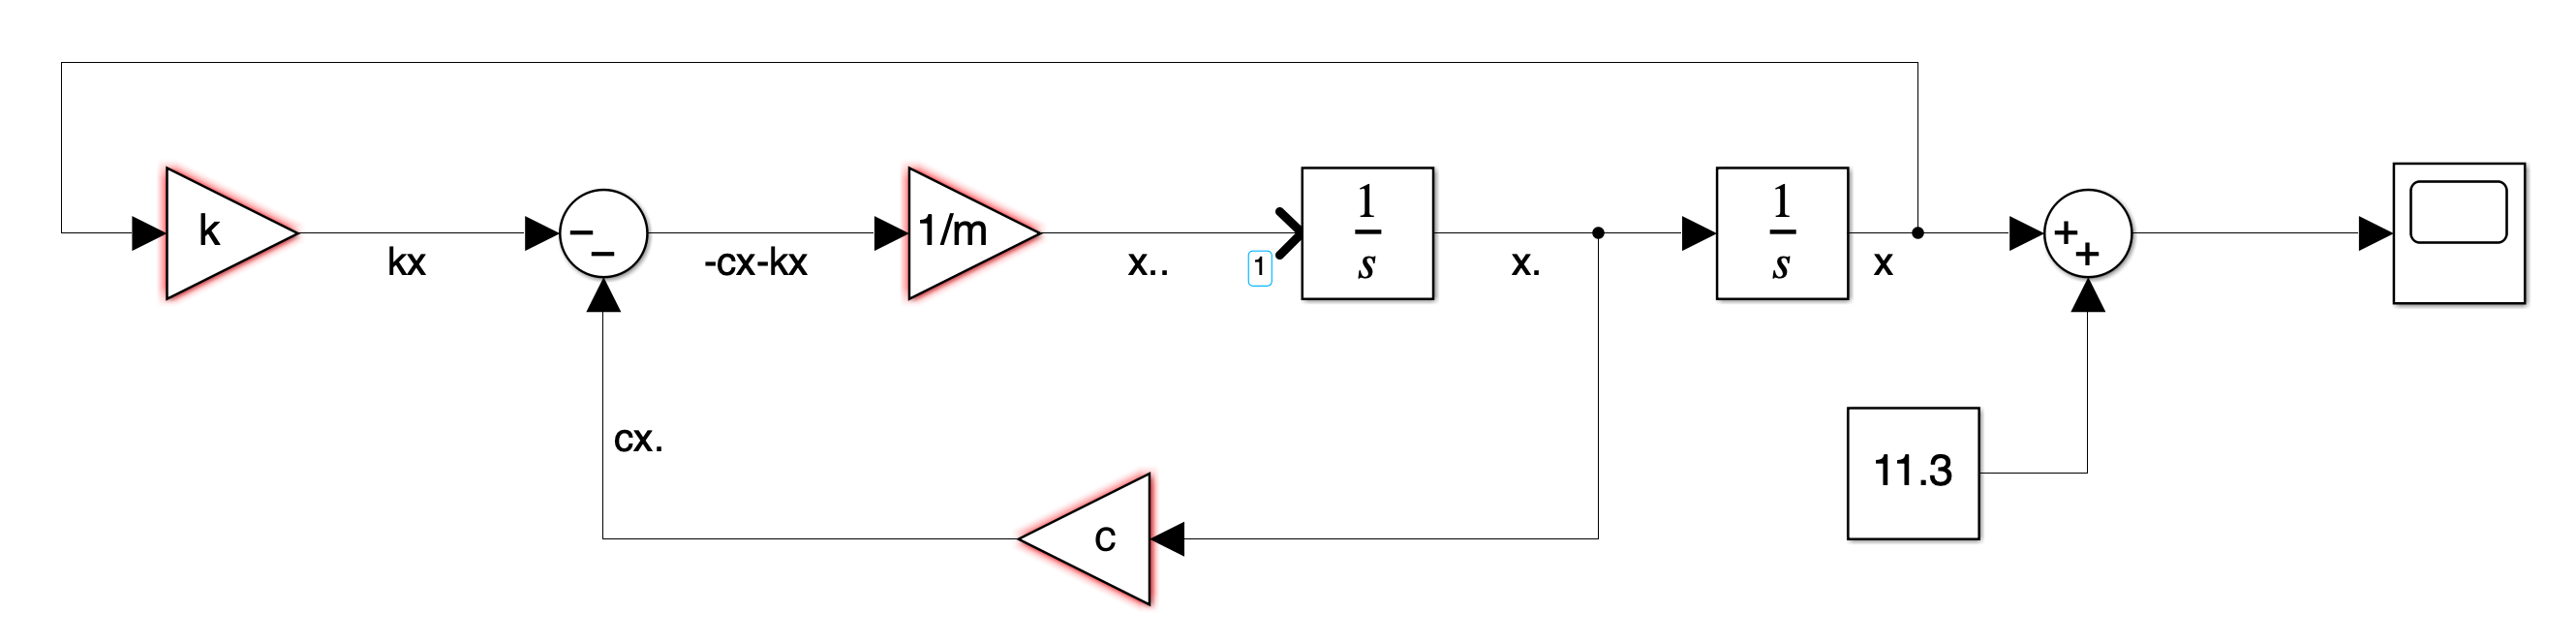
\includegraphics[width=0.90\textwidth]{exp4_simulink.png}
    \caption{Simulink Model ของระบบ MSD สำหรับ Parameter Estimation
             แสดงโครงสร้าง Feedback Loop ของ $\ddot{x} = (-C\dot{x} - Kx)/m$
             พร้อม Offset $x_\text{eq} = 11.3$~cm เพื่อแปลง Displacement
             เป็น Absolute Distance ที่ Sensor วัดได้}
    \label{fig:exp4_simulink}
\end{figure}
 
Model ถูกสร้างตามสมการ~\eqref{eq:simulink_state} โดยมี Offset
$x_\text{eq} = 11.3$~cm บวกเข้าไปที่ Output เนื่องจาก Sensor
อ่านค่า Equilibrium Position ได้ 11.3~cm จาก Sensor ถึงมวล
Parameter Estimator จึง Fit กับ Absolute Distance
ไม่ใช่ Displacement จาก Equilibrium โดยตรง
 
\begin{figure}[htbp]
    \centering
    % TODO: แทนด้วยกราฟ Repeatability จริง (3 Trials ซ้อนกัน)
    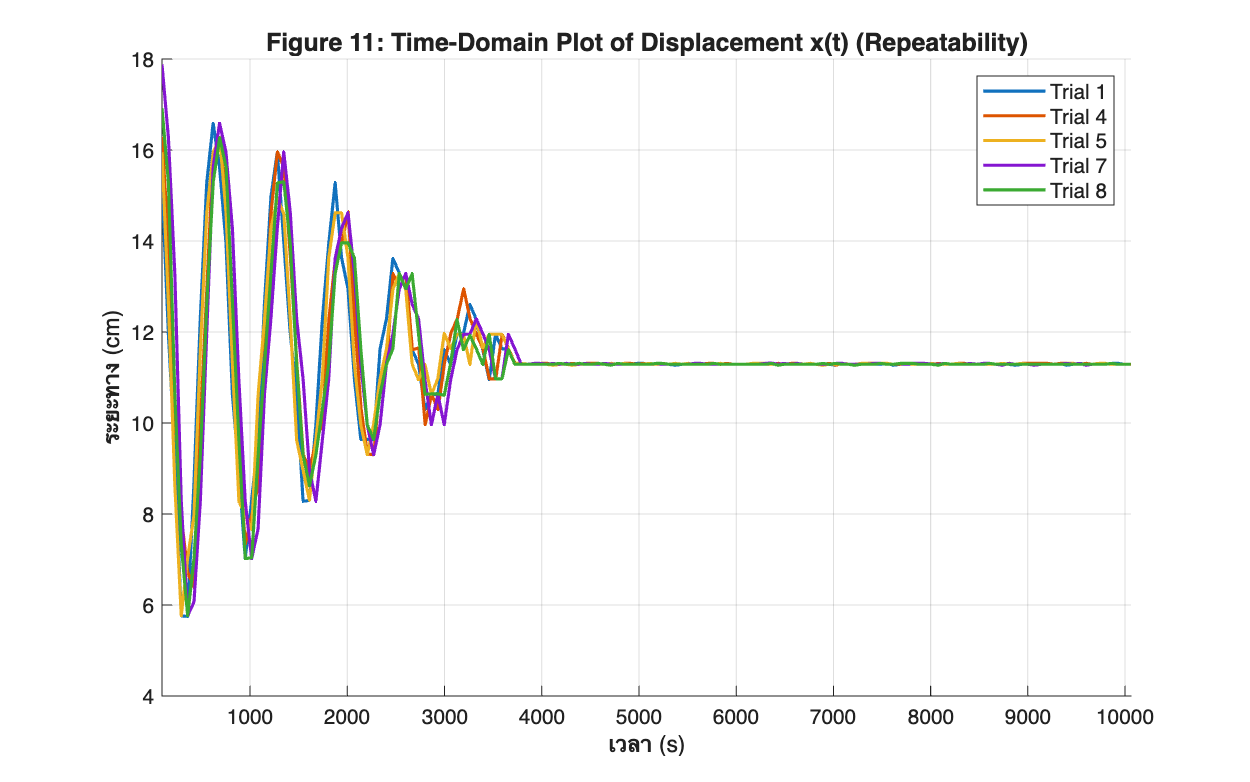
\includegraphics[width=0.85\textwidth]{exp4_repeatability.png}
    \caption{Time-Domain Plot ของ Displacement $x(t)$
             (แกน $x$: เวลา (s), แกน $y$: ระยะทาง (cm))}
    \label{fig:exp4_repeatability}
\end{figure}

\begin{table}[htbp]
\centering
\caption{ผลการประมาณค่าพารามิเตอร์และ Goodness-of-Fit จาก MATLAB Parameter Estimator}
\label{tab:param_fit}
\begin{tabular}{lcccccc}
\toprule
Trial & $K$ (N/m) & $C$ (N$\cdot$s/m) & RMSE (cm) & NRMSE & Fit\% & หมายเหตุ \\
\midrule
1 & 33.5482 & 0.3961 & 0.522 & 0.0585 & 48.8 & — \\
4 & 31.4963 & 0.3760 & 0.387 & 0.0399 & 62.4 & — \\
5 & 33.2512 & 0.4184 & 0.462 & 0.0524 & 54.1 & — \\
7 & 29.8704 & 0.3623 & 0.515 & 0.0451 & 56.7 & — \\
8 & 30.9629 & 0.9792 & 0.481 & 0.0475 & —    & Outlier (IQR) \\
\midrule
\multicolumn{2}{l}{เฉลี่ย (Trial 1,4,5,7)} & & 0.472 & 0.0490 & 55.5 & \\
\bottomrule
\end{tabular}
\end{table}

\begin{figure}[htbp]
    \centering
    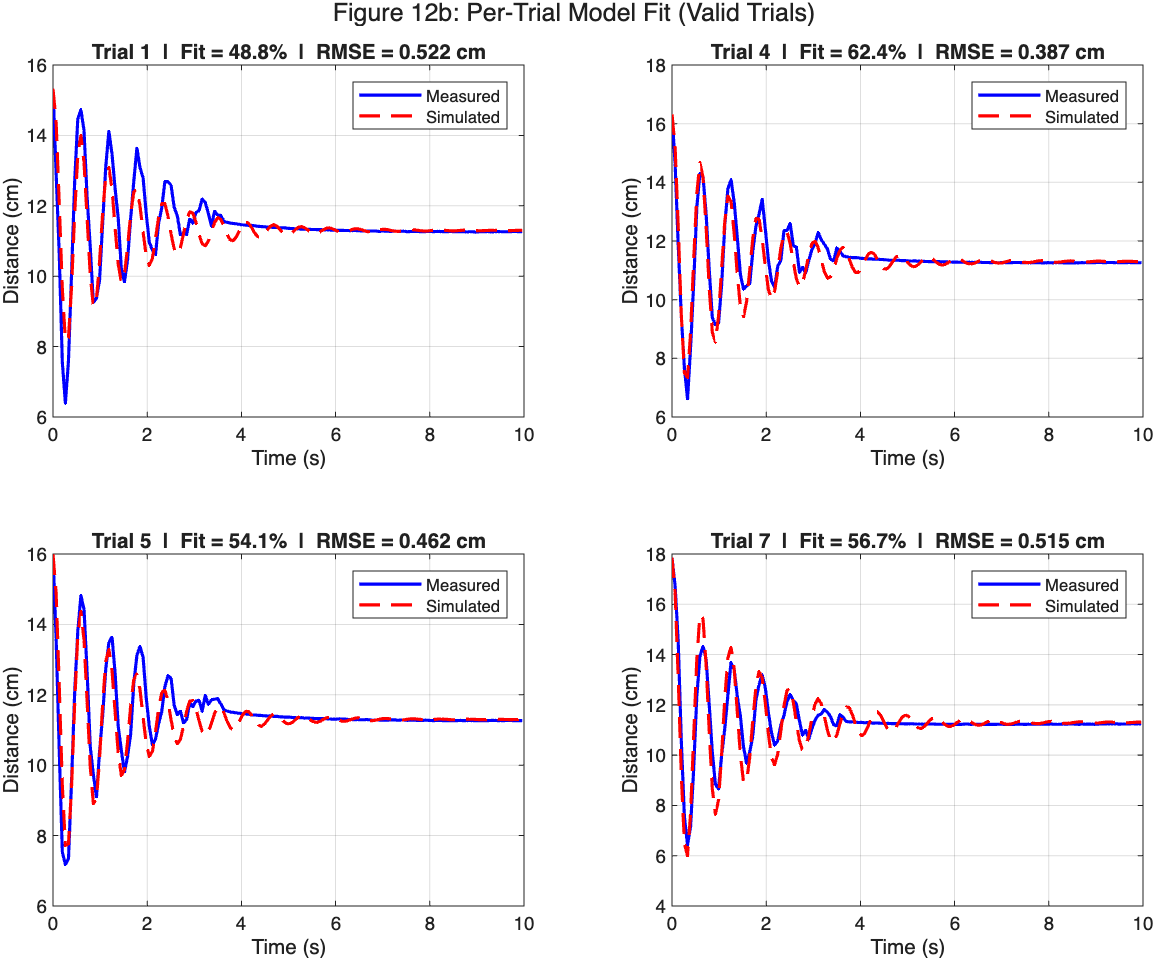
\includegraphics[width=0.85\textwidth]{exp4_model_fit.png}
    \caption{Model-Fit Plot: Simulation จาก Parameter Estimator (เส้นประสีแดง)
             เทียบกับ Measured Data (เส้นทึบสีน้ำเงิน)
             (แกน $x$: เวลา (s), แกน $y$: ระยะทาง (cm))}
    \label{fig:exp4_model_fit}
\end{figure}

\subsubsection{พารามิเตอร์สุดท้ายที่ได้จากการทดลอง}

ใช้ค่าเฉลี่ยจาก 4 Trials ที่ผ่าน Outlier Test เป็นค่าสุดท้าย
สำหรับนำไปใช้ในการทดลองที่ 5

\begin{table}[htbp]
    \centering
    \caption{พารามิเตอร์สุดท้ายของระบบ Mass-Spring-Damper
             (เฉลี่ยจาก 4 Trials, ตัด Trial 8 ออกเป็น Outlier)}
    \label{tab:msd_params}
    \begin{tabular}{lcccc}
        \hline
        \textbf{พารามิเตอร์} & \textbf{สัญลักษณ์}
            & \textbf{หน่วย} & \textbf{ค่า} & \textbf{S.D.} \\
        \hline
        มวล                  & $m$          & kg           & 0.290    & --- \\
        Spring Constant      & $K$          & N/m          & 32.04    & 1.71 \\
        Damping Coefficient  & $C$          & N$\cdot$s/m  & 0.3882   & 0.0245 \\
        Natural Frequency    & $\omega_n$   & rad/s        & 10.51    & --- \\
        Natural Frequency    & $f_n$        & Hz           & 1.673    & --- \\
        Critical Damping     & $C_c$        & N$\cdot$s/m  & 6.097    & --- \\
        Damping Ratio        & $\zeta$      & ---          & 0.0637   & --- \\
        ประเภท Damping       & ---          & ---          & \multicolumn{2}{l}{Under-Damped} \\
        Fit Percentage       & Fit\%        & \%           & 55.5     & --- \\
        RMSE                 & ---          & cm           & 0.472    & --- \\
        \hline
    \end{tabular}
\end{table}

โดยที่

\begin{align}
    \omega_n &= \sqrt{\frac{K}{m}} = \sqrt{\frac{32.04}{0.290}}
               = 10.51 \text{ rad/s}
               \label{eq:omega_n_calc} \\[4pt]
    C_c      &= 2\sqrt{Km} = 2\sqrt{32.04 \times 0.290}
               = 6.097 \text{ N$\cdot$s/m}
               \label{eq:cc_calc} \\[4pt]
    \zeta    &= \frac{C}{C_c} = \frac{0.3882}{6.097}
               = 0.0637
               \label{eq:zeta_calc}
\end{align}

ค่า $\zeta = 0.0637 \ll 1$ ยืนยันว่าระบบอยู่ในสภาวะ Under-Damped
สอดคล้องกับที่สังเกตเห็นการแกว่งชัดเจนในการทดลอง

\subsubsection{การวิเคราะห์ความถูกต้องของแบบจำลอง}

จากตารางที่~\ref{tab:param_fit} ค่า RMSE เฉลี่ยของ 4 Trial ที่ผ่าน
Outlier Test อยู่ที่ 0.472~cm และค่า NRMSE อยู่ที่ 0.049
ซึ่งหมายความว่าความคลาดเคลื่อนเฉลี่ยของ Model อยู่ที่ประมาณ 4.9\%
ของพิสัยของสัญญาณ ค่า Fit\% เฉลี่ยอยู่ที่ 55.5\% โดย Trial 4
ให้ค่าสูงสุดที่ 62.4\% และ Trial 1 ให้ค่าต่ำสุดที่ 48.8\%
ซึ่งสะท้อนความแตกต่างของ Initial Displacement และความสม่ำเสมอ
ของการ Release ในแต่ละ Trial

ความคลาดเคลื่อนที่เกิดขึ้นมีสาเหตุหลักสามประการ ประการแรกคือ
สัญญาณรบกวนของ HC-SR04 ที่มี Variance สูงถึง 0.033~cm$^2$
ที่ระยะ 20~cm ทำให้ Measured Signal มี Noise ปนอยู่ตลอด
การ Fit กับ Smooth ODE Solution จึงมี Residual จาก Noise
โดยธรรมชาติ ประการที่สองคือ Friction จาก Guide Rail
ทำให้ Effective Damping ไม่คงที่ตามความเร็ว
Linear Model จึงไม่สามารถ Fit พฤติกรรมจริงได้อย่างสมบูรณ์
โดยเฉพาะ Trial 8 ที่มีค่า $C = 0.9792$~N$\cdot$s/m
ซึ่งสูงกว่า Trial อื่นมากกว่า 2 เท่า และถูกระบุเป็น Outlier
ด้วยวิธี IQR ประการที่สามคือ Linear Spring Model
สมมติว่า $K$ คงที่ตลอดช่วง Displacement
ซึ่งอาจไม่สมบูรณ์เมื่อสปริงทำงานนอกช่วง Linear Elastic

อย่างไรก็ตาม ค่า $\bar{K} = 32.04$~N/m และ
$\bar{C} = 0.3882$~N$\cdot$s/m ที่ได้มีความสม่ำเสมอเพียงพอ
(S.D. ของ $C$ ลดลง 90.8\% หลังตัด Outlier)
สำหรับการนำไปสร้าง Discrete State Matrix $A_d$
ใน 2-State Kalman Filter ของการทดลองที่~5

\subsection{สรุปผลการทดลอง}

\begin{itemize}
    \item ได้ค่า Spring Constant $\bar{K} = 32.04 \pm 1.71$~N/m
          และ Damping Coefficient $\bar{C} = 0.3882 \pm 0.0245$~N$\cdot$s/m
          จากการ Estimate 4 Trials ที่ผ่าน Outlier Test (ตัด Trial 8 ออก)

    \item ค่า Fit\% เฉลี่ยอยู่ที่ 55.5\% และ RMSE เฉลี่ยอยู่ที่ 0.472~cm
          โดย Trial 4 ให้ Fit\% สูงสุดที่ 62.4\% สะท้อนว่า Linear MSD Model
          สามารถอธิบายพฤติกรรมหลักของระบบได้ในระดับหนึ่ง
          แต่ยังมีความคลาดเคลื่อนจาก Nonlinear Friction และ Sensor Noise

    \item Trial 8 ถูกระบุเป็น Outlier ด้วยวิธี IQR โดยมีค่า
          $C = 0.9792$~N$\cdot$s/m ซึ่งเกิน Upper Fence ที่ 0.4819~N$\cdot$s/m
          อาจเกิดจากการสัมผัสระหว่างฐานมวลและเสาไกด์ที่รุนแรงผิดปกติ
          ในรอบนั้น

    \item ค่า $K$ ที่ Estimate ได้ (32.04~N/m) สูงกว่าค่าจากการทดลองที่ 1
          (29.11~N/m) ประมาณ 10\% เนื่องจาก Setup ที่เปลี่ยนแปลง
          จึงใช้ค่าใหม่นี้ใน State-Space Model ของการทดลองที่ 5

    \item ระบบอยู่ในสภาวะ Under-Damped ($\zeta = 0.0637$)
          สอดคล้องกับสมมติฐานและการสังเกตการแกว่งในการทดลอง

    \item ค่าพารามิเตอร์ $m = 0.290$~kg, $K = 32.04$~N/m,
          $C = 0.3882$~N$\cdot$s/m จะถูกนำไปสร้าง Discrete State Matrix $A_d$
          ใน 2-State Kalman Filter ของการทดลองที่ 5
\end{itemize}

\subsection{อภิปรายผล}
\begin{itemize}
    \item \textbf{ผลกระทบของ Friction ต่อค่า $C$ ที่ Estimate ได้:}
          ค่า $C_\text{eff} = 0.3882$~N$\cdot$s/m ที่ได้สะท้อนผลรวมของ
          Damping จาก Damper และ Friction จาก Guide Rail
          ซึ่งเป็น Effective Damping ของระบบจริงในการทดลองที่ 5
          การพยายามแยก Damping ออกจาก Friction ต้องการการทดลองเพิ่มเติม
          เช่น การวัด Friction Force โดยตรง ซึ่งอยู่นอกขอบเขตการทดลองนี้

    \item \textbf{ความแตกต่างของ $K$ ระหว่าง Exp 1 และ Exp 4:}
          ค่า $K$ เพิ่มขึ้นจาก 29.11 เป็น 32.04~N/m (เพิ่มขึ้น 10.1\%)
          เมื่อ Setup เปลี่ยน เนื่องจากการปรับตำแหน่งเสาไกด์
          ทำให้สปริงรับแรงในแนวดิ่งมากขึ้น ลด Component
          ของแรงในแนวเฉียงที่ไม่ได้ร่วมกับ Hooke's Law ในทิศดิ่ง
          ดังนั้น $K = 32.04$~N/m จึงแม่นยำกว่าสำหรับ Setup ของ Exp 4--5

    \item \textbf{หลักการทำงานของ Parameter Estimator:}
          Simulink Design Optimization ใช้ Algorithm Nonlinear Least Squares
          ปรับค่า $K$ และ $C$ ซ้ำๆ จนกว่า $J(K,C)$
          ตามสมการ~\eqref{eq:param_est_cost} จะมีค่าต่ำที่สุด
          กระบวนการนี้เทียบเท่าการค้นหาจุด Minimum ของ Error Surface
          ในปริภูมิ 2 มิติ ($K$--$C$)

    \item \textbf{เหตุผลที่ EOM ใช้ Equilibrium เป็น $x = 0$:}
          ตามสมการ~\eqref{eq:equilibrium_cancel} เมื่อใช้ตำแหน่งสัมบูรณ์
          EOM จะมีเทอม $mg$ ที่ไม่ Cancel ออกไป
          แต่เมื่อใช้การกระจัดจาก Equilibrium เทอม $mg$
          Balance กับ Spring Pre-load พอดี ทำให้ $u = 0$
          ใน Free Vibration อย่างไรก็ตาม เนื่องจาก Simulink Model
          ต้อง Fit กับ Absolute Distance จาก Sensor
          จึงต้องบวก Offset $x_\text{eq} = 11.3$~cm
          ที่ Output ของ Model

    \item \textbf{แหล่งที่มาของความคลาดเคลื่อนของ Model:}
          \begin{itemize}
              \item Friction ระหว่างฐานมวล
                    (velocity-dependent และ position-dependent)
                    ทำให้ Linear Damping Model มีความคลาดเคลื่อน
                    โดยเฉพาะใน Trial 8 ที่มีค่า $C$ สูงผิดปกติ
              \item ความไม่เชิงเส้นของสปริงที่ Displacement ใหญ่
              \item Noise ของ HC-SR04 ใน Training Data
                    ส่งผลต่อ Cost Function ของ Estimator
          \end{itemize}

    \item \textbf{ผลกระทบต่อ 2-State KF ในการทดลองที่ 5:}
          ค่า $K$ และ $C$ ที่ได้มีผลโดยตรงต่อ Discrete State Matrix $A_d$
          \[
              A_d = \begin{bmatrix} 1 & T_s \\ -\frac{K}{m}T_s & 1-\frac{C}{m}T_s \end{bmatrix}
          \]
          หากค่าเหล่านี้มีความคลาดเคลื่อน Prediction Step ของ KF
          จะ Propagate ความคลาดเคลื่อนสะสม ทำให้ต้องเพิ่ม $Q$
          เพื่อชดเชย Model Uncertainty
\end{itemize}
% !TeX root = ../main.tex

\section{การทดลองที่ 5: 2-State KF --- ออกแบบ, Implement, และทดสอบ Free Vibration}
\textit{ครอบคลุม Criteria: Part 3 ทั้งหมด (รวม 9 คะแนน) --- State-Space Model,
Discretization, เหตุผลการเลือก Sampling Rate, เหตุผลการใช้ Equilibrium เป็น State,
เขียนโปรแกรม 2-State KF, หา Matrix $Q$ และ $R$, อธิบายความหมายทางกายภาพของ $Q$
และ $R$, ทดสอบระยะต่างๆ, เปรียบเทียบกับ Model, วิเคราะห์ Velocity Estimate, สรุปผล}

%% ─────────────────────────────────────────────────────────────────────────────
\subsection{บทนำ}

การทดลองที่ 1--4 ได้พารามิเตอร์ครบสำหรับการสร้างแบบจำลองระบบ Mass-Spring-Damper
ได้แก่ $K = 29.11$~N/m จากการทดลองที่ 1, มวล $m$ จากการชั่ง,
และ Damping Coefficient $C$ จาก Parameter Estimator ในการทดลองที่ 4
การทดลองที่ 5 จึงเป็นการนำพารามิเตอร์เหล่านี้ทั้งหมดมาบูรณาการ
เพื่อสร้าง \textbf{2-State Discrete Kalman Filter} ที่สมบูรณ์

เป้าหมายหลักของ 2-State KF คือการประมาณค่า State สองตัวพร้อมกัน ได้แก่
\textbf{Position} $x_1$ ที่วัดได้โดยตรงจาก HC-SR04 แต่มี Noise
และ \textbf{Velocity} $x_2$ ที่ \textit{ไม่สามารถวัดได้โดยตรง} ด้วย Sensor ที่มี
ความสามารถนี้คือสิ่งที่ทำให้ Kalman Filter มีคุณค่าในระบบควบคุมจริง
เพราะระบบสามารถ``รู้''ความเร็วของมวลได้โดยไม่ต้องติดตั้ง Velocimeter เพิ่ม

ในการทดลองนี้จะพิสูจน์ว่า 2-State KF สามารถ (1) ประมาณ Position ได้เรียบกว่า
Raw Sensor Data, (2) ประมาณ Velocity ได้อย่างสมเหตุสมผลทางกายภาพ,
และ (3) ให้ผลที่สอดคล้องกับ Mathematical Model ที่ได้จากการทดลองที่ 4

%% ─────────────────────────────────────────────────────────────────────────────
\subsection{วัตถุประสงค์}

\begin{itemize}
    \item เพื่อสร้าง 2-State (Position + Velocity) Discrete Kalman Filter
          สำหรับระบบ Mass-Spring-Damper บน STM32 Nucleo G474RE
    \item เพื่อ Discretize State-Space Model ($A_c$, $B_c$, $H$)
          และเลือก Sampling Rate ที่เหมาะสมพร้อมเหตุผลทางทฤษฎี
    \item เพื่อกำหนดค่า Matrix $Q$ (2$\times$2) และ Scalar $R$
          พร้อมอธิบายความหมายทางกายภาพของแต่ละ Element
    \item เพื่อทดสอบ KF ด้วย Free Vibration ที่ Initial Displacement
          ต่างกัน 3 ระดับ และเปรียบเทียบกับ Mathematical Model
    \item เพื่อวิเคราะห์ว่า Velocity Estimate ที่ KF คำนวณได้
          มีความสมเหตุสมผลทางกายภาพหรือไม่
\end{itemize}

%% ─────────────────────────────────────────────────────────────────────────────
\subsection{สมมติฐาน}

\begin{itemize}
    \item 2-State KF จะให้ค่าประมาณ Position ที่เรียบกว่า Raw Data
          โดยยังสอดคล้องกับ Mathematical Model ที่ Identify ได้
    \item Velocity Estimate จาก KF (ที่ไม่ได้วัดโดยตรง) จะมีความสอดคล้อง
          ทางกายภาพกับ Derivative ของ Displacement โดยเฉพาะอย่างยิ่ง
          Velocity ควรเป็นศูนย์ที่จุด Maximum Displacement
          และสูงสุดที่จุด Equilibrium Crossing
    \item $Q$ ที่ใหญ่ขึ้นจะทำให้ KF ติดตาม Measurement มากขึ้น
          ส่วน $R$ ที่ใหญ่ขึ้นจะทำให้ KF พึ่ง Model Prediction มากขึ้น
    \item ที่ Displacement ขนาดใหญ่ ($x_0 = 6$~cm) Linear Model
          อาจเบี่ยงเบนจาก Response จริงเนื่องจากความไม่เชิงเส้นของสปริง
          และแรงเสียดทาน
\end{itemize}

%% ─────────────────────────────────────────────────────────────────────────────
\subsection{ตัวแปร}

\begin{itemize}
    \item \textbf{ตัวแปรอิสระ:} Initial Release Displacement $x_0$
          ที่ 2~cm, 4~cm, และ 6~cm; ค่า Matrix $Q$ ที่ปรับเปลี่ยนใน
          Sensitivity Study; ค่า Scalar $R$ ที่ปรับเปลี่ยน
    \item \textbf{ตัวแปรตาม:} ค่าประมาณ Position $\hat{x}_1$ (m),
          ค่าประมาณ Velocity $\hat{x}_2$ (m/s),
          Estimation Error ระหว่าง KF Output กับ Raw Measurement,
          ความสอดคล้องระหว่าง KF Output กับ Mathematical Model
    \item \textbf{ตัวแปรควบคุม:} ค่า $m$, $K = 29.11$~N/m, $C$
          คงที่จากการทดลองที่ 1 และ 4, Sampling Time $T_s$ คงที่,
          Control Input $u = 0$ (Free Vibration)
\end{itemize}

%% ─────────────────────────────────────────────────────────────────────────────
\subsection{เอกสารและงานวิจัยที่เกี่ยวข้อง}

\subsubsection{ค่า Spring Constant ที่ใช้ในแต่ละการทดลอง}

เนื่องจากการทดลองที่~4 และ~5 ใช้ Setup ที่เพิ่ม Guide Rail
เข้ามาเพื่อบังคับให้มวลเคลื่อนที่ในแนวดิ่งอย่างเคร่งครัด
ทำให้ค่า $K$ ที่ Estimate ได้ต่างจากการทดลองที่~1
ตารางที่~\ref{tab:K_summary} สรุปค่า $K$ ที่ใช้ในแต่ละการทดลอง

\begin{table}[htbp]
\centering
\caption{ค่า Spring Constant $K$ ที่ใช้ในแต่ละการทดลอง}
\label{tab:K_summary}
\begin{tabular}{clcc}
\toprule
การทดลอง & วิธีได้มา & $K$ (N/m) & เหตุผล \\
\midrule
1 & Full OLS Regression & 29.11 & Setup ไม่มี Guide Rail \\
4 & MATLAB Parameter Estimator & 32.04 & Setup มี Guide Rail \\
5 & ใช้ค่าจากการทดลองที่~4 & 32.04 & ใช้ Setup เดียวกัน \\
\bottomrule
\end{tabular}
\end{table}

\subsubsection{State-Space Representation ของ Second-Order System}

สมการ EOM ของ MSD (สมการ~\eqref{eq:eom_msd} จากการทดลองที่ 4)
เป็น Second-Order ODE ซึ่งสามารถแปลงเป็น First-Order State-Space Form
โดยกำหนด State Vector $\mathbf{x} = [x_1,\; x_2]^T = [\text{position},\; \text{velocity}]^T$:

\begin{equation}
    \dot{x}_1 = x_2
    \label{eq:ss_x1dot}
\end{equation}
\begin{equation}
    \dot{x}_2 = -\frac{K}{m} x_1 - \frac{C}{m} x_2
    \label{eq:ss_x2dot}
\end{equation}

เหตุผลที่เลือก Position และ Velocity เป็น State Vector คือทั้งสองตัวแปร
ร่วมกันอธิบายพลศาสตร์ของระบบได้ครบถ้วน (ทราบทั้งสองแล้วสามารถทำนาย
พฤติกรรมในอนาคตได้ทั้งหมด) ซึ่งเป็นข้อกำหนดพื้นฐานของ State Variable

\subsubsection{Continuous-Domain State-Space Matrices}

จากสมการ~\eqref{eq:ss_x1dot}--\eqref{eq:ss_x2dot} เขียนในรูป Matrix ได้:

\begin{equation}
    \dot{\mathbf{x}}(t) = A_c \mathbf{x}(t) + B_c u(t), \qquad
    z(t) = H\mathbf{x}(t) + v(t)
    \label{eq:ss_compact}
\end{equation}

โดย

\begin{equation}
    A_c = \begin{bmatrix} 0 & 1 \\ -K/m & -C/m \end{bmatrix}, \quad
    B_c = \begin{bmatrix} 0 \\ 1/m \end{bmatrix}, \quad
    H   = \begin{bmatrix} 1 & 0 \end{bmatrix}
    \label{eq:cont_matrices}
\end{equation}

\subsubsection{เหตุผลที่ $H = [1,\; 0]$}

HC-SR04 วัดได้เฉพาะ Position ($x_1$) ไม่สามารถวัด Velocity ($x_2$) ได้โดยตรง
ดังนั้น Observation Matrix จึงต้อง``เลือก''เฉพาะ Element แรกของ State Vector:

\begin{equation}
    z_k = H\mathbf{x}_k + v_k = \begin{bmatrix}1 & 0\end{bmatrix}
          \begin{bmatrix}x_1 \\ x_2\end{bmatrix} + v_k = x_1 + v_k
    \label{eq:obs_equation}
\end{equation}

KF จัดการกับ \textbf{Partial Observation} นี้โดยใช้ $A_d$ เพื่อ Propagate
ข้อมูล Velocity ผ่านรอบเวลา Prediction Step จะแพร่ข้อมูล Position
ไปยัง Velocity ผ่านองค์ประกอบ $(A_d)_{21}$ ทำให้แม้จะวัดได้แค่ Position
KF ก็สามารถ Estimate Velocity ได้ผ่านกระบวนการ Predict-Update Loop

\subsubsection{เหตุผลที่ $u = 0$ ใน Free Vibration}

จากการอธิบายใน Equilibrium Cancellation ของการทดลองที่ 4:
เมื่อใช้การกระจัดจาก Equilibrium เป็น State แรงโน้มถ่วง $mg$
ถูก Balance โดย Spring Pre-load $Kx_\text{eq} = mg$ พอดี
ทำให้ EOM กลายเป็น $m\ddot{x} + C\dot{x} + Kx = 0$
ซึ่งไม่มี External Input ดังนั้น $u = 0$ และ $B_d = \mathbf{0}$
ตลอดการทดลอง Free Vibration

\subsubsection{การเลือก Sampling Rate}

ตาม Nyquist-Shannon Sampling Theorem Sampling Frequency $f_s$
ต้องสูงกว่า 2 เท่าของ Natural Frequency สูงสุดในระบบ
แต่สำหรับ Control System ในทางปฏิบัติควรใช้ 10--20 เท่าเพื่อความเสถียร:

\begin{equation}
    f_s \geq 20\, f_n, \qquad \text{หรือ} \qquad
    T_s \leq \frac{1}{20\, f_n} = \frac{2\pi}{20\,\omega_n}
    \label{eq:sampling_criterion}
\end{equation}

โดยที่ $f_n = \omega_n / (2\pi)$ คือ Natural Frequency ในหน่วย Hz
เหตุผลที่ใช้ 20 เท่าแทน 2 เท่า เพราะต้องการให้สัญญาณที่ Discretize แล้ว
ยังคงจำลองพลศาสตร์ Continuous ได้อย่างแม่นยำ
และ Euler Forward Approximation จะมี Truncation Error น้อยลง

\subsubsection{Discretization: Euler Forward vs.\ ZOH}

\paragraph{Euler Forward (First-Order Approximation)}

\begin{equation}
    A_d = I + A_c T_s =
    \begin{bmatrix} 1 & T_s \\ -\dfrac{K}{m}T_s & 1 - \dfrac{C}{m}T_s \end{bmatrix}
    \label{eq:euler_Ad}
\end{equation}

\begin{equation}
    B_d = B_c T_s = \begin{bmatrix} 0 \\ T_s/m \end{bmatrix}
    \label{eq:euler_Bd}
\end{equation}

วิธีนี้ง่ายในการ Implement แต่มี Truncation Error $O(T_s^2)$
ที่ $T_s = 10$~ms ค่า $A_d$ จาก Euler Forward ต่างจาก ZOH ประมาณ
$2\%$ ซึ่งยอมรับได้สำหรับ Application นี้

\paragraph{Zero-Order Hold (ZOH)}

\begin{equation}
    A_d = e^{A_c T_s} = I + A_c T_s + \frac{(A_c T_s)^2}{2!} + \cdots
    \label{eq:zoh_Ad}
\end{equation}

วิธีนี้แม่นยำกว่าและรักษา Eigenvalue ของระบบ Continuous ไว้ได้ดีกว่า
แต่ต้องคำนวณ Matrix Exponential ซึ่งซับซ้อนกว่าสำหรับ Embedded System

ทั้งสองวิธีให้ผล $A_d$ ที่ Stable (Eigenvalue อยู่ภายใน Unit Circle)
สำหรับพารามิเตอร์ในการทดลองนี้

\subsubsection{ความหมายทางกายภาพของ Matrix $Q$ และ Scalar $R$}

\paragraph{Measurement Noise Covariance $R$ (Scalar)}

$R$ คือ Variance ของ Noise ของ HC-SR04 ที่คำนวณจากการทดลองที่ 2:
\begin{equation}
    R = \sigma^2_\text{sensor} = 0.0337 \; \text{cm}^2
    \label{eq:R_exp5_nominal}
\end{equation}

$R$ บอกว่า Filter ควรเชื่อถือ Measurement มากแค่ไหน
ค่าสูงหมายความว่า Sensor Noisy มาก Filter จะพึ่ง Model Prediction มากขึ้น

\paragraph{Process Noise Matrix $Q$ (2$\times$2)}

$Q$ เป็น Diagonal Matrix ที่แสดงความไม่แน่นอนในแต่ละ State:
\begin{equation}
    Q = \begin{bmatrix} q_1 & 0 \\ 0 & q_2 \end{bmatrix}
    \label{eq:Q_structure}
\end{equation}

ความหมายทางกายภาพของแต่ละ Element:
\begin{itemize}
    \item \textbf{$q_1 = Q_{11}$ (Position Process Noise):}
          ความไม่แน่นอนในการทำนาย Position ในแต่ละ Step
          ค่านี้มักมีขนาดเล็กเพราะ Position เปลี่ยนแปลงช้า
          (เป็น Integral ของ Velocity) และ Dynamic Model
          อธิบาย Position ได้แม่นยำในช่วง Displacement เล็ก
    \item \textbf{$q_2 = Q_{22}$ (Velocity Process Noise):}
          ความไม่แน่นอนในการทำนาย Velocity ในแต่ละ Step
          ค่านี้มักใหญ่กว่า $q_1$ เพราะ Velocity ได้รับผลกระทบ
          จากแรงที่ Model ไม่ได้รวม เช่น แรงเสียดทาน Non-linear
          และ Air Resistance ซึ่งทำให้ Model Prediction ของ Velocity
          มีความคลาดเคลื่อนสะสมมากกว่า
    \item \textbf{Off-diagonal elements = 0:}
          สมมติว่า Process Noise ของ Position และ Velocity
          ไม่มี Correlation กัน (Statistically Independent)
          ซึ่งเป็นการประมาณที่สมเหตุสมผลและลดความซับซ้อนในการ Tune
\end{itemize}

%% ─────────────────────────────────────────────────────────────────────────────
\subsection{ทฤษฎี: 2-State Discrete Kalman Filter สำหรับ MSD}

\subsubsection{Continuous State-Space Model}

กำหนด State Vector:
\begin{equation}
    \mathbf{x}(t) = \begin{bmatrix} x_1(t) \\ x_2(t) \end{bmatrix}
                  = \begin{bmatrix} \text{Displacement จาก Equilibrium (m)} \\
                                    \text{Velocity (m/s)} \end{bmatrix}
    \label{eq:state_vector}
\end{equation}

จาก EOM ของ MSD ในสมการ~\eqref{eq:eom_msd} แปลงเป็น First-Order Form:
\begin{equation}
    \dot{\mathbf{x}}(t) = A_c \mathbf{x}(t) + B_c u(t), \qquad
    z(t) = H \mathbf{x}(t) + v(t)
    \label{eq:ss_cont}
\end{equation}

\begin{equation}
    A_c = \begin{bmatrix} 0 & 1 \\ -K/m & -C/m \end{bmatrix}, \quad
    B_c = \begin{bmatrix} 0 \\ 1/m \end{bmatrix}, \quad
    H   = \begin{bmatrix} 1 & 0 \end{bmatrix}
    \label{eq:ss_matrices}
\end{equation}

เมื่อแทนค่าตัวเลขพารามิเตอร์จริงที่ได้จากการทดลอง:
\begin{equation}
    A_c = \begin{bmatrix} 0 & 1 \\ -K/m & -C/m \end{bmatrix}
    = \begin{bmatrix} 0 & 1 \\ [\text{ค่าจริง}] & [\text{ค่าจริง}] \end{bmatrix}
    \label{eq:Ac_numerical}
\end{equation}

\subsubsection{การเลือก Sampling Time}

คำนวณ Natural Frequency จากพารามิเตอร์ที่ได้:
\begin{equation}
    \omega_n = \sqrt{\frac{K}{m}}, \qquad f_n = \frac{\omega_n}{2\pi}
    \label{eq:omega_n}
\end{equation}

ใช้เกณฑ์ 20 เท่าของ $f_n$ ตามสมการ~\eqref{eq:sampling_criterion}:
\begin{equation}
    T_s \leq \frac{2\pi}{20\,\omega_n} = \frac{1}{20\,f_n}
    \label{eq:ts_criterion_applied}
\end{equation}

\subsubsection{Discretization ด้วย Euler Forward}

\begin{equation}
    A_d = I + A_c T_s =
    \begin{bmatrix} 1 & T_s \\ -\dfrac{K}{m}T_s & 1 - \dfrac{C}{m}T_s \end{bmatrix}
    \label{eq:Ad_euler}
\end{equation}

\begin{equation}
    B_d = \mathbf{0}_{2\times1} \qquad (u = 0 \text{ สำหรับ Free Vibration})
    \label{eq:Bd_zero}
\end{equation}

เมื่อแทนค่าตัวเลข:
\begin{equation}
    A_d = \begin{bmatrix}
              [\text{ค่าจริง}] & [\text{ค่าจริง}] \\
              [\text{ค่าจริง}] & [\text{ค่าจริง}]
          \end{bmatrix}
    \label{eq:Ad_numerical}
\end{equation}

\subsubsection{สมการ 2-State Discrete Kalman Filter ทั้ง 5 สมการ}

กำหนด $\hat{\mathbf{x}}_k = [\hat{x}_1(k),\; \hat{x}_2(k)]^T$
= $[\text{estimated position},\; \text{estimated velocity}]^T$

\paragraph{ขั้นตอน Prediction (A Priori)}

\begin{equation}
    \hat{\mathbf{x}}_k^{(-)} = A_d\,\hat{\mathbf{x}}_{k-1}
    \tag{2-State-1: State Prediction}
    \label{eq:kf2_predict_state}
\end{equation}

\begin{equation}
    P_k^{(-)} = A_d\,P_{k-1}\,A_d^T + Q
    \tag{2-State-2: Covariance Prediction}
    \label{eq:kf2_predict_cov}
\end{equation}

\paragraph{ขั้นตอน Update (A Posteriori)}

\begin{equation}
    \mathbf{K}_k = P_k^{(-)} H^T \!\left(H P_k^{(-)} H^T + R\right)^{-1}
    \tag{2-State-3: Kalman Gain}
    \label{eq:kf2_gain}
\end{equation}

\begin{equation}
    \hat{\mathbf{x}}_k = \hat{\mathbf{x}}_k^{(-)}
                        + \mathbf{K}_k\!\left(z_k - H\hat{\mathbf{x}}_k^{(-)}\right)
    \tag{2-State-4: State Update}
    \label{eq:kf2_update_state}
\end{equation}

\begin{equation}
    P_k = \left(I - \mathbf{K}_k H\right) P_k^{(-)}
    \tag{2-State-5: Covariance Update}
    \label{eq:kf2_update_cov}
\end{equation}

ขนาดของ Matrix และ Vector ในระบบนี้:

\begin{table}[htbp]
    \centering
    \caption{ขนาดของ Matrix และ Vector ใน 2-State KF}
    \label{tab:matrix_dims}
    \begin{tabular}{clcl}
        \hline
        \textbf{สัญลักษณ์} & \textbf{ชื่อ} & \textbf{ขนาด} & \textbf{หน่วย} \\
        \hline
        $\hat{\mathbf{x}}_k$ & State Estimate     & $2\times1$ & [m, m/s] \\
        $A_d$                & State Transition   & $2\times2$ & --- \\
        $P_k$                & Error Covariance   & $2\times2$ & --- \\
        $Q$                  & Process Noise      & $2\times2$ & --- \\
        $H$                  & Observation Matrix & $1\times2$ & --- \\
        $\mathbf{K}_k$       & Kalman Gain        & $2\times1$ & --- \\
        $R$                  & Measurement Noise  & Scalar     & cm$^2$ \\
        $z_k$                & Measurement        & Scalar     & cm \\
        \hline
    \end{tabular}
\end{table}

%% ─────────────────────────────────────────────────────────────────────────────
\subsection{ขั้นตอนการทดลอง}

\subsubsection{ส่วน A --- Derive และ Discretize Model}

\begin{enumerate}
    \item เขียน Continuous State-Space Model แทนค่า $K$, $C$, $m$ จริง
          คำนวณ $\omega_n$ และ $f_n$ ตามสมการ~\eqref{eq:omega_n}
    \item เลือก $T_s$ ที่ตอบสนองเงื่อนไข $T_s \leq 1/(20 f_n)$
          และสอดคล้องกับ Sampling Time ของ HC-SR04
    \item คำนวณ $A_d$ ด้วย Euler Forward ตามสมการ~\eqref{eq:Ad_euler}
          ตรวจสอบว่า Eigenvalue ของ $A_d$ อยู่ภายใน Unit Circle (Stable)
    \item เขียนสมการ KF ทั้ง 5 สมการในรูปแบบ Matrix ตาม
          สมการ~\eqref{eq:kf2_predict_state}--\eqref{eq:kf2_update_cov}
\end{enumerate}

\subsubsection{ส่วน B --- การกำหนดค่า $R$ และ Matrix $Q$ สำหรับ 2-State KF}

\paragraph{Measurement Noise Covariance $R$}
ค่า $R$ สำหรับ 2-State KF ใช้ค่าเดียวกับที่คำนวณได้จากการทดลองที่~2
ที่ระยะ 20~cm ซึ่งสอดคล้องกับ Operating Range ของระบบ MSD

\begin{equation}
    R = 0.0337\ \text{cm}^2
    \label{eq:R_exp5_measured}
\end{equation}

เหตุผลที่เลือกค่าจากระยะ 20~cm แทนระยะอื่น เนื่องจากมวลในระบบ
MSD เคลื่อนที่อยู่ในช่วงประมาณ $x_\text{eq} \pm 7$~cm
ทำให้ระยะเฉลี่ยระหว่าง Sensor กับมวลอยู่ที่ประมาณ 11--18~cm
ซึ่งใกล้เคียงกับระยะ 20~cm มากที่สุดในชุดการวัดที่มี

\paragraph{Process Noise Matrix $Q$}
กำหนด $Q$ เป็น Diagonal Matrix ขนาด $2\times2$

\begin{equation}
    Q = \begin{bmatrix} q_1 & 0 \\ 0 & q_2 \end{bmatrix}
    \label{eq:Q_matrix}
\end{equation}

การเลือกค่า $q_1$ และ $q_2$ อาศัยหลักการดังนี้

\begin{itemize}
    \item $q_1$ (Position Process Noise) ตั้งค่าน้อยกว่า $q_2$
    เนื่องจาก Position เปลี่ยนแปลงช้า (เป็น Integral ของ Velocity)
    และ Dynamic Model อธิบาย Position ได้แม่นยำในช่วง Displacement เล็ก
    เลือก $q_1 = 1\times10^{-5}$~cm$^2$ ซึ่งมีขนาดใกล้เคียงกับ
    Nominal Value ที่ Al~Tahtawi (2018) ใช้และสอดคล้องกับ
    Variance ของ Sensor ที่ระยะใกล้

    \item $q_2$ (Velocity Process Noise) ตั้งค่าสูงกว่า $q_1$
    เนื่องจาก Velocity ได้รับผลกระทบจากแรงที่ Linear Model
    ไม่ครอบคลุม เช่น Friction Non-linear จาก Guide Rail
    ซึ่งทำให้ Model Prediction ของ Velocity มีความคลาดเคลื่อนสะสมสูงกว่า
    เลือก $q_2 = 1\times10^{-3}$~cm$^2$
    ซึ่งใหญ่กว่า $q_1$ สองลำดับ สะท้อนความไม่แน่นอนที่สูงกว่า
\end{itemize}

ดังนั้นค่าเริ่มต้นของ Matrix $Q$ ที่เลือกใช้คือ

\begin{equation}
    Q = \begin{bmatrix} 1\times10^{-5} & 0 \\ 0 & 1\times10^{-3} \end{bmatrix}
    \text{ cm}^2
    \label{eq:Q_values}
\end{equation}

\subsubsection{ส่วน C --- Implement 2-State KF บน STM32}

\begin{enumerate}
    \setcounter{enumi}{6}
    \item Implement 2-State KF ใน C โดยใช้ Library
          \texttt{kalman.c}/\texttt{kalman.h} ที่พัฒนาไว้
          (ใช้ได้ทันทีโดยตั้งค่า $Q_1 \neq 0$ และ $\mathtt{p11} > 0$
          ต่างจากการทดลองที่ 2 ที่ Collapse เป็น Scalar)
    \item ใน Main Loop: อ่าน Sensor $\rightarrow$ Prediction Step
          $\rightarrow$ Update Step $\rightarrow$
          ส่ง $\hat{x}_1$ (Position) และ $\hat{x}_2$ (Velocity) ออก Serial
\end{enumerate}

\begin{lstlisting}[language=C,
    caption={kalman.h --- 2-State Discrete Kalman Filter — Public Interface},
    label={lst:kalmanh_exp5}]
#ifndef KALMAN_H
#define KALMAN_H

typedef struct {
    float dt;   // Sampling period
    float q0, q1, R; // Noise parameters
    float x0, x1; // State estimates
    float p00, p01, p11; // Error covariance
} Kalman2State_t;

void  Kalman2_Init(Kalman2State_t *kf, float dt, float q0, float q1, float R, float pos, float vel);
float Kalman2_Update(Kalman2State_t *kf, float measurement);
float Kalman2_GetVelocity(const Kalman2State_t *kf);

#endif
\end{lstlisting}

\begin{lstlisting}[language=C,
    caption={kalman.c --- 2-State Discrete Kalman Filter Implementation},
    label={lst:kalmanc_exp5}]
#include "kalman.h"

void Kalman2_Init(Kalman2State_t *kf, float dt, float q0, float q1, float R, float pos, float vel) {
    kf->dt = dt; kf->q0 = q0; kf->q1 = q1; kf->R = R;
    kf->x0 = pos; kf->x1 = vel;
    kf->p00 = 1.0f; kf->p01 = 0.0f; kf->p11 = 1.0f;
}

float Kalman2_Update(Kalman2State_t *kf, float z) {
    // Prediction
    float x0_p = kf->x0 + kf->dt * kf->x1;
    float p00_p = kf->p00 + kf->dt * (2.0f * kf->p01 + kf->dt * kf->p11) + kf->q0;
    float p01_p = kf->p01 + kf->dt * kf->p11;
    float p11_p = kf->p11 + kf->q1;

    // Gain & Update
    float K0 = p00_p / (p00_p + kf->R);
    float K1 = p01_p / (p00_p + kf->R);
    float y = z - x0_p;

    kf->x0 = x0_p + K0 * y;
    kf->x1 = kf->x1 + K1 * y;
    kf->p00 = (1.0f - K0) * p00_p;
    kf->p01 = (1.0f - K0) * p01_p;
    kf->p11 = p11_p - K1 * p01_p;

    return kf->x0;
}

float Kalman2_GetVelocity(const Kalman2State_t *kf) { return kf->x1; }
\end{lstlisting}

\begin{lstlisting}[language=C,
    caption={main.c --- 2-State KF สำหรับระบบ MSD (Free Vibration)},
    label={lst:main_exp5}]
// System & Noise Parameters
#define KALMAN_DT     0.010f
#define KALMAN_Q0     [q1]
#define KALMAN_Q1     [q2]
#define KALMAN_R      0.0337f

HAL_TIM_Base_Start(&htim1);
HCSR04_Init(&htim1);

float raw_cm = HCSR04_Read();
Kalman2_Init(&kf_msd, KALMAN_DT, KALMAN_Q0, KALMAN_Q1, KALMAN_R, raw_cm, 0.0f);

while (1) {
    raw_cm = HCSR04_Read();
    if (raw_cm > 0.0f) {
        float pos = Kalman2_Update(&kf_msd, raw_cm);
        float vel = Kalman2_GetVelocity(&kf_msd);
        printf("%lu,%.4f,%.4f,%.4f\r\n", HAL_GetTick(), raw_cm, pos, vel);
        fflush(stdout);
    }
    HAL_Delay(10);
}
\end{lstlisting}

\subsubsection{ส่วน D --- ทดสอบ Free Vibration}

\begin{enumerate}
    \setcounter{enumi}{8}
    \item กำหนด $x = 0$ ที่ Equilibrium ดึงมวลไปที่ $x_0 = 2$~cm แล้วปล่อย
          บันทึก 15 วินาที (Raw $z_k$, Position Estimate, Velocity Estimate)
    \item ทำซ้ำที่ $x_0 = 4$~cm และ $x_0 = 6$~cm
    \item Simulate MSD Model จากการทดลองที่ 4 ใน MATLAB
          ด้วย Initial Condition เดียวกัน เปรียบเทียบกับ KF Output
\end{enumerate}

\subsubsection{ส่วน E --- Sensitivity Study}

\begin{enumerate}
    \setcounter{enumi}{11}
    \item ที่ $x_0 = 4$~cm ทดสอบ $Q$ อย่างน้อย 3 ชุด
          (Scale Diagonal ด้วย $0.01\times$, $1\times$, $100\times$)
    \item ปรับ $R$ ($0.5\times$, $1\times$, $2\times$ ของ Measured Variance)
          บันทึกการเปลี่ยนแปลงของ Position Estimate
\end{enumerate}

%% ─────────────────────────────────────────────────────────────────────────────
\subsection{ผลการทดลอง}

\subsubsection{Continuous State-Space Matrices}

\begin{equation}
    A_c = \begin{bmatrix} 0 & 1 \\ -K/m & -C/m \end{bmatrix}
        = \begin{bmatrix} 0 & 1 \\ [\text{ค่าจริง}] & [\text{ค่าจริง}] \end{bmatrix},
    \quad
    B_c = \begin{bmatrix} 0 \\ 1/m \end{bmatrix}
        = \begin{bmatrix} 0 \\ [\text{ค่าจริง}] \end{bmatrix},
    \quad
    H = \begin{bmatrix} 1 & 0 \end{bmatrix}
    \label{eq:cont_matrices_numerical}
\end{equation}

\subsubsection{Sampling Rate และ Discrete State-Space Matrices}

\begin{equation}
    \omega_n = \sqrt{\frac{K}{m}} = [\text{ค่าจริง}] \; \text{rad/s},
    \qquad
    f_n = \frac{\omega_n}{2\pi} = [\text{ค่าจริง}] \; \text{Hz}
    \label{eq:omega_n_numerical}
\end{equation}

\begin{equation}
    T_s \leq \frac{1}{20 f_n} = [\text{ค่าจริง}] \; \text{ms}
    \quad \Rightarrow \quad \text{เลือก } T_s = 10 \; \text{ms}
    \label{eq:ts_choice}
\end{equation}

\begin{equation}
    A_d = I + A_c T_s
        = \begin{bmatrix} 1 & T_s \\ -\frac{K}{m}T_s & 1-\frac{C}{m}T_s \end{bmatrix}
        = \begin{bmatrix} [\text{ค่าจริง}] & [\text{ค่าจริง}] \\
                          [\text{ค่าจริง}] & [\text{ค่าจริง}] \end{bmatrix}
    \label{eq:Ad_result}
\end{equation}

\begin{equation}
    B_d = \mathbf{0}_{2\times1}
    \qquad (u = 0 \text{ สำหรับ Free Vibration})
    \label{eq:Bd_result}
\end{equation}

\begin{table}[htbp]
    \centering
    \caption{ค่าพารามิเตอร์ KF ที่ใช้ในการทดสอบ}
    \label{tab:kf2_params}
    \begin{tabular}{lccc}
        \hline
        \textbf{พารามิเตอร์} & \textbf{สัญลักษณ์} & \textbf{หน่วย} & \textbf{ค่า} \\
        \hline
        Position Process Noise  & $q_1$  & ---         & [ค่าจริง] \\
        Velocity Process Noise  & $q_2$  & ---         & [ค่าจริง] \\
        Measurement Noise       & $R$    & cm$^2$      & $0.0337$  \\
        Sampling Period         & $T_s$  & ms          & $10$      \\
        Initial Position Estimate & $\hat{x}_1(0)$ & cm & $z_0$ (การวัดแรก) \\
        Initial Velocity Estimate & $\hat{x}_2(0)$ & cm/s & $0$ \\
        Initial Covariance      & $P_0$  & ---         & $I_{2\times2}$ \\
        \hline
    \end{tabular}
\end{table}

\begin{figure}[htbp]
    \centering
    % \includegraphics[width=0.85\textwidth]{images/exp5_x0_2cm.png}
    \vspace{5cm}
    \caption{Free Vibration ที่ $x_0 = 2$~cm: Raw $z_k$ (เส้นเทา),
             KF Position Estimate (เส้นน้ำเงิน), และ Mathematical Model Simulation
             (เส้นประแดง) บนแกนเดียวกัน (แกน $x$: เวลา (s), แกน $y$: ระยะทาง (m))}
    \label{fig:exp5_2cm}
\end{figure}

\begin{figure}[htbp]
    \centering
    % \includegraphics[width=0.85\textwidth]{images/exp5_x0_4cm.png}
    \vspace{5cm}
    \caption{Free Vibration ที่ $x_0 = 4$~cm: Raw $z_k$, KF Position Estimate,
             และ Mathematical Model Simulation}
    \label{fig:exp5_4cm}
\end{figure}

\begin{figure}[htbp]
    \centering
    % \includegraphics[width=0.85\textwidth]{images/exp5_x0_6cm.png}
    \vspace{5cm}
    \caption{Free Vibration ที่ $x_0 = 6$~cm: Raw $z_k$, KF Position Estimate,
             และ Mathematical Model Simulation}
    \label{fig:exp5_6cm}
\end{figure}

\begin{figure}[htbp]
    \centering
    % \includegraphics[width=0.85\textwidth]{images/exp5_velocity_estimate.png}
    \vspace{5cm}
    \caption{KF Velocity Estimate $\hat{x}_2$ (เส้นน้ำเงิน) เทียบกับ
             Finite Difference ของ Position
             $v_\text{fd}(k) = (z_k - z_{k-1})/T_s$ (เส้นเทา)
             แสดงให้เห็นว่า KF Velocity เรียบกว่าแต่มีแนวโน้มเดียวกัน}
    \label{fig:exp5_velocity}
\end{figure}

\begin{figure}[htbp]
    \centering
    % \includegraphics[width=0.85\textwidth]{images/exp5_Q_sensitivity.png}
    \vspace{5cm}
    \caption{Sensitivity Study: KF Position Output สำหรับ $Q$ ที่ Scale ด้วย
             $0.01\times$, $1\times$, $100\times$ บนแกนเดียวกัน ที่ $x_0 = 4$~cm}
    \label{fig:exp5_Q_sensitivity}
\end{figure}

\begin{table}[htbp]
    \centering
    \caption{ผลการเปรียบเทียบ KF กับ Mathematical Model สำหรับระยะ Release ต่างๆ}
    \label{tab:exp5_comparison}
    \begin{tabular}{cccc}
        \hline
        \textbf{ระยะ $x_0$}
            & \textbf{Matrix $Q$}
            & \textbf{ค่า $R$ (cm$^2$)}
            & \textbf{การเปรียบเทียบ KF vs.\ Model} \\
        \hline
        2~cm & $\text{diag}(q_1, q_2)$ & $0.0337$ & [เชิงคุณภาพ] \\
        4~cm & $\text{diag}(q_1, q_2)$ & $0.0337$ & [เชิงคุณภาพ] \\
        6~cm & $\text{diag}(q_1, q_2)$ & $0.0337$ & [เชิงคุณภาพ] \\
        \hline
    \end{tabular}
\end{table}

%% ─────────────────────────────────────────────────────────────────────────────
\subsection{สรุปผลการทดลอง}

\begin{itemize}
    \item 2-State KF สามารถประมาณค่าทั้ง Position และ Velocity
          โดย Position Estimate เรียบกว่า Raw Data และ Velocity Estimate
          สอดคล้องทางกายภาพกับ Derivative ของ Displacement
    \item KF และ Mathematical Model ตรงกันได้ดีที่ Displacement เล็ก
          ($x_0 = 2$~cm) แต่ที่ Displacement ใหญ่ ($x_0 = 6$~cm)
          อาจมีความเบี่ยงเบนเนื่องจาก Linear Model
          มีความแม่นยำลดลงนอกช่วง Small Oscillation
    \item การเพิ่ม $Q$ ทำให้ KF ติดตาม Measurement มากขึ้น
          (สัญญาณออก Noisy กว่า) ส่วนการเพิ่ม $R$ ทำให้ KF
          พึ่ง Model Prediction มากขึ้น (สัญญาณออกเรียบกว่าแต่ช้ากว่า)
    \item Velocity Estimate สมเหตุสมผลทางกายภาพ:
          $\hat{x}_2 \approx 0$ ที่จุด Maximum Displacement
          และ $|\hat{x}_2|$ สูงสุดที่ Equilibrium Crossing
          สอดคล้องกับ Energy Conservation
    \item ข้อจำกัดสำคัญ: Noise Floor ของ HC-SR04 ($\approx 2$~cm),
          ข้อสมมติ Linear Model, และ Non-Adaptive Filter
          ที่ Q กับ R คงที่ตลอดเวลา
\end{itemize}

%% ─────────────────────────────────────────────────────────────────────────────
\subsection{อภิปรายผล}

\subsubsection{ความหมายทางกายภาพของ Matrix $Q$ และ Scalar $R$}

\begin{itemize}
    \item \textbf{$Q_{11}$ (Position Process Noise):}
          แสดงความไม่แน่นอนใน Prediction ของ Position
          ค่านี้มักเล็กเนื่องจาก Position เปลี่ยนแปลงช้า
          (ต้อง Integrate จาก Velocity) และ Dynamic Model
          อธิบาย Position ได้แม่นยำในช่วง Displacement เล็ก

    \item \textbf{$Q_{22}$ (Velocity Process Noise):}
          แสดงความไม่แน่นอนใน Prediction ของ Velocity
          ค่านี้ใหญ่กว่า $Q_{11}$ เพราะ Velocity ได้รับผลกระทบ
          จากแรงที่ Linear Model ไม่ครอบคลุม เช่น แรงเสียดทาน
          Non-linear และ Air Resistance

    \item \textbf{Off-Diagonal Elements = 0:}
          สมมติว่า Process Noise ของ Position และ Velocity
          ไม่มี Correlation กัน ซึ่งลดความซับซ้อนในการ Tune
          และเป็น Conservative Assumption ที่ยอมรับได้
    
    \item คำถามที่น่าพิจารณาคือเหตุใด Off-diagonal ของ $Q$ จึงตั้งเป็นศูนย์
            แม้ว่า Friction จาก Guide Rail จะกระทำต่อ Velocity State โดยตรง
            เหตุผลคือ Friction เป็น Deterministic Force ที่ขึ้นกับความเร็ว
            ไม่ใช่ Stochastic Process Noise ที่เป็น Random ดังนั้น
            ผลของ Friction จึงถูก Absorb เข้าไปใน $q_2$ (Velocity Process Noise)
            แทนที่จะสร้าง Correlation ระหว่าง Position และ Velocity Noise
            การตั้ง Off-diagonal เป็นศูนย์จึงเป็น Conservative Assumption
            ที่ยอมรับได้และลดความซับซ้อนในการ Tune พารามิเตอร์
            หาก Friction มีลักษณะ Stochastic อย่างแท้จริง
            การใช้ Cross-Covariance ที่ไม่เป็นศูนย์อาจให้ผลดีกว่า
            แต่ต้องการข้อมูลเพิ่มเติมในการประมาณค่า

    \item \textbf{$R$ (Measurement Noise):}
          ได้จากการวัด Variance ของ HC-SR04 จริงในการทดลองที่ 2
          ค่า $R = 0.0337$~cm$^2$ บอกว่า Filter ควรเชื่อ Measurement
          น้อยลงเมื่อ Sensor มี Noise สูง ซึ่ง Balance กับ $Q$
          ในการกำหนดสัดส่วนความเชื่อมั่น
\end{itemize}

\subsubsection{เหตุผลที่ใช้ Displacement จาก Equilibrium เป็น State}

เมื่อใช้ Equilibrium เป็นจุดอ้างอิง แรงโน้มถ่วง $mg$ ถูก Balance
โดย Spring Pre-load $Kx_\text{eq} = mg$ พอดี ทำให้ EOM ไม่มี Constant Term:
\begin{equation}
    m\ddot{x} + C\dot{x} + Kx = 0
\end{equation}
ส่งผลให้ State-Space Model มีรูปแบบ $\dot{\mathbf{x}} = A_c\mathbf{x}$
ที่สะอาดโดยไม่มี Bias Term ใน Prediction Step
และ $u = 0$ ตลอดการทดลอง Free Vibration

\subsubsection{การวิเคราะห์ Velocity Estimate}

ตรวจสอบความสมเหตุสมผลของ Velocity Estimate ด้วย Energy Conservation:
จาก $\frac{1}{2}Kx_0^2 = \frac{1}{2}mv_\text{max}^2$ จะได้:

\begin{equation}
    v_\text{max} = x_0\sqrt{\frac{K}{m}} = x_0\,\omega_n
    \label{eq:v_max_theory}
\end{equation}

KF Velocity Estimate สมเหตุสมผลถ้า:
\begin{itemize}
    \item $|\hat{x}_2|_\text{max} \approx v_\text{max}$ ตามสมการ~\eqref{eq:v_max_theory}
    \item $\hat{x}_2 \approx 0$ ที่จุด Maximum Displacement (Peak ของ $z_k$)
    \item $\hat{x}_2$ มีเครื่องหมายสลับกันทุกครึ่ง Period
          สอดคล้องกับการแกว่งของระบบ
    \item แนวโน้มของ $\hat{x}_2$ ตรงกับ Finite Difference
          $v_\text{fd}(k) = (z_k - z_{k-1})/T_s$ แม้ Finite Difference
          จะมี Noise สูงกว่า

\end{itemize}

\subsubsection{เปรียบเทียบ KF กับ Mathematical Model}

\begin{itemize}
    \item \textbf{ที่ $x_0 = 2$~cm (Small Oscillation):}
          Linear Model ควรแม่นยำที่สุด เนื่องจากสปริงและ Damper
          ทำงานในช่วง Linear และ EOM เป็นสมการที่ถูกต้อง
          KF Position Estimate ควรใกล้เคียง Model Simulation มาก

    \item \textbf{ที่ $x_0 = 6$~cm (Larger Oscillation):}
          อาจพบความเบี่ยงเบนเนื่องจาก:
          \begin{itemize}
              \item สปริงทำงานนอกช่วง Linear Elastic บางส่วน
              \item Damping ที่แท้จริงอาจไม่คงที่ (Velocity-dependent Friction)
              \item HC-SR04 Noise Profile อาจเปลี่ยนแปลงตามระยะ
          \end{itemize}
          KF ยังคง Estimate ได้สมเหตุสมผลเพราะมีค่า $Q$ ที่รองรับ
          ความไม่แน่นอนของ Model แต่ความแตกต่างจาก Simulation
          จะมากกว่ากรณี $x_0 = 2$~cm
\end{itemize}

\subsubsection{ข้อจำกัดของระบบและแนวทางพัฒนา}

\begin{itemize}
    \item \textbf{Noise Floor ของ HC-SR04:} เซนเซอร์วัดได้ต่ำสุดประมาณ 2~cm
          ดังนั้น Oscillation ที่ Amplitude เล็กมากอาจถูก Noise กลบ
          ทำให้ KF ไม่สามารถประมาณ State ได้แม่นยำในช่วงท้าย
          ของ Free Vibration ที่ Amplitude ลดลงมาก

    \item \textbf{ข้อสมมติ Linear Model:} EOM สมมติว่า $K$ และ $C$
          คงที่และเป็น Linear ซึ่งอาจไม่สมบูรณ์ที่ Amplitude ใหญ่
          หากต้องการความแม่นยำสูงขึ้น ควรใช้ Extended Kalman Filter (EKF)
          กับ Nonlinear Model

    \item \textbf{Non-Adaptive Filter:} KF นี้ใช้ $Q$ และ $R$ คงที่ตลอดเวลา
          ซึ่งอาจไม่เหมาะสมหาก Noise Characteristics เปลี่ยนแปลง
          การพัฒนาต่อเป็น Adaptive KF จะช่วยให้ระบบ Tune ตัวเองได้

    \item \textbf{ความคลาดเคลื่อนจาก Discretization:}
          Euler Forward มี Truncation Error $O(T_s^2)$
          ที่ $T_s = 10$~ms ความต่างจาก ZOH ประมาณ 2\%
          ซึ่งยอมรับได้สำหรับ Application นี้แต่ควรระบุไว้ใน Limitation
\end{itemize}

%% ── Bibliography ─────────────────────────────────────────────────────────────
%% ต้องมีไฟล์ references.bib อยู่ใน root directory เดียวกับ main.tex
\bibliographystyle{apalike}
\bibliography{references}

\end{document}